%=============================================================================
%\documentclass[11pt,twoside]{article}
\documentclass[11pt,a4paper,twoside,bibtotoc]{scrartcl}
%\documentclass[twoside,11pt]{article}
%\usepackage{jnm}
%=============================================================================
\usepackage{a4wide}
\usepackage{amsfonts}
\usepackage{amsmath}
\usepackage{theorem}
\usepackage{jkmath}
\usepackage{subfigure}
\usepackage{natbib}
\usepackage{algorithm}
\usepackage{algorithmic}
%\usepackage{showkeys}
%\usepackage{psfig}
%\usepackage{lscape}
%\usepackage{color}
%\usepackage{graphics}
\usepackage{graphicx}

\renewcommand{\topfraction}{1}
\renewcommand{\textfraction}{0}
\setcounter{totalnumber}{4}

%============================================================================


\numberwithin{equation}{section}
\numberwithin{table}{section}
\numberwithin{figure}{section}

%\newlength{\temp}
%\setcounter{totalnumber}{10}
%\setcounter{topnumber}{10}

%============================================================================

\title{
%{\rm\normalsize Short Note}\\
Fast Summation on the sphere}

\date{\today}

\author{
Jens Keiner\thanks{keiner@math.uni-luebeck.de, University of
  L\"ubeck, Institute of Mathematics, D--23560 L\"ubeck} \and
Stefan Kunis\thanks{kunis@math.uni-luebeck.de, University of
  L\"ubeck, Institute of Mathematics, D--23560 L\"ubeck} \and
  Daniel Potts\thanks{potts@math.uni-luebeck.de, University of
  L\"ubeck, Institute of Mathematics, D--23560 L\"ubeck} 
}

%=============================================================================
\begin{document}
\maketitle

\begin{abstract}
\medskip

%\noindent
%2000 {\it Mathematics Subject Classification}. 65F10, 65F15, 65T40.

\noindent
{\it Key words and phrases}.  
\end{abstract}

%-----------------------------------------------------------------------------
\section{Introduction}
\label{sect:1}

\begin{proposition}[Addition Theorem]
  \label{Basics:AdditionTheorem}
  For every $\Ln{2}{\twosphere}$-orthonormal basis 
  $\set{H_{k}^n}_{n=-k}^{k}$ of $\mathcal{H}_k$, we have
  \begin{equation}
    \nonumber
    \sum_{n=-k}^{k} \fun{H_{k}^n}{\V{\xi}} \overline{\fun{H_{k}^n}{\V{\eta}}} =
    \frac{2k+1}{4\pi}\fun{P_k}{\V{\xi} \: \V{\eta}}.
  \end{equation}
\end{proposition}


\section{Fast Summation}

An essential task in modern spherical approximation methods is the fast evaluation of linear combinations $f$ of (space localizing) spherical radial basis functions $K$,  
\begin{equation}
  \label{Applications:KernelSum}
  f: \twosphere \rightarrow \R,\ \fun{f}{\xi} := \sum_{l = 0}^{L-1} 
    b_{l} \fun{K}{\V{\eta}_{l} \cdot \V{\xi}} \quad \paren{\V{\xi} \in \twosphere}
\end{equation}
on a set of \emph{target nodes} 
$$
  \mathcal{X} := \pset{\V{\xi}_{d} \in \twosphere}{|}{d=0,\ldots,D-1,\ D \in \N}
$$ 
with 
$$
  \mathcal{Y} := \pset{\V{\eta}_{l} \in \twosphere}{|}{l = 0,\ldots,L-1,\ L \in \N}
$$
being the set of \emph{source nodes}, $b_{l} \in \R$ and $\fun{K}{\V{\eta} \: \cdot}$ a \emph{radial spherical basis function} or \emph{$\V{\eta}$-zonal function} 
\[
  \fun{K}{\V{\eta} \: \cdot}: \twosphere \rightarrow \R,\ \V{\xi} \mapsto \fun{K}{\V{\eta} \cdot \V{\xi}} \quad \paren{\V{\xi} \in \twosphere}.\]

The naive approach, i.e. evaluating \eqref{Applications:KernelSum} for every $\V{\xi}_{d} \in \mathcal{X}$ clearly leads to an $\bigo{L\:D}$ algorithm. For large $L$ and $D$ the computational effort becomes quickly unaffordable.
The \emph{panel clustering} method introduced in \cite{FrGlSch98} reduces the computational effort to evaluate \eqref{Applications:KernelSum} based on the traditional method of dividing the evaluation into near- and far-field. For every kernel $\fun{K}{\V{\eta} \: \cdot}$, the near-field contribution is calculated exactly whereas the contribution of the far-field may be approximated coarsly due to the supposed rapid decay of $\fun{K}{\V{\eta} \: \cdot}$. 

The approach presented here is a a cutoff in frequency-domain. Using \eqref{Basics:Kernel}, we obtain
%$$
%  \fun{f}{\xi} = \sum_{l = 0}^{L-1} b_{l} \sum_{k=0}^{\infty} \beta_{k} \fun{P_k}{\V{\eta}_{l} \cdot \V{\xi}}.
%$$
%Now using the Addition Theorem \ref{} we can write
\[
  \fun{K}{\V{\eta}_{l} \cdot \V{\xi}} = \sum_{k=0}^{\infty} \sum_{n=-k}^k \fun{K^{\wedge}}{k} \fun{Y_{k}^n}{\V{\xi}} \overline{\fun{Y_{k}^n}{\V{\eta}_{l}}}
\]
and by truncating at a finite index $M \in \NZ$, i.e. defining
\begin{equation}
  \label{Applications:TruncatedSeries}
  \fun{K_{M}}{\V{\eta}_{l} \cdot \V{\xi}} := 
  \sum_{k=0}^{M} \sum_{n=-k}^k \fun{K^{\wedge}}{k} \fun{Y_{k}^n}{\V{\xi}} \overline{\fun{Y_{k}^n}{\V{\eta}_{l}}}
\end{equation}
we obtain
\begin{equation}
  \nonumber
  \begin{split}
    \fun{f}{\xi} \approx \fun{f_{M}}{\xi} & := \sum_{l = 0}^{L-1} b_{l} \fun{K_{M}}{\V{\eta}_{l} \cdot \V{\xi}} \\
                 &       = \sum_{l = 0}^{L-1} b_{l} \sum_{k=0}^{M} \sum_{n=-k}^k \fun{K^{\wedge}}{k}
                           \fun{Y_{k}^n}{\V{\xi}} \overline{\fun{Y_{k}^n}{\V{\eta}_{l}}} \\
                 &       = \sum_{k=0}^{M} \sum_{n=-k}^k \paren{\sum_{l = 0}^{L-1} b_{l}
                           \overline{\fun{Y_{k}^n}{\V{\eta}_{l}}}} \fun{K^{\wedge}}{k} \fun{Y_{k}^n}{\V{\xi}}.
  \end{split}                           
\end{equation}
Evaluating the sums
\begin{equation}
\label{Applications:AdjointNDSFT}
  \tilde{b}_{k}^n := \sum_{l = 0}^{L-1} b_{l} \overline{\fun{Y_{k}^n}{\V{\eta}_{l}}} \quad \paren{k = 0,\ldots,M; n = -k,\ldots,k}
\end{equation}
corresponds to an adjoint NDSFT and we arrive at
\[
  \fun{f_{M}}{\xi} = \sum_{k=0}^{M} \sum_{n=-k}^k \tilde{b}_{k}^n \fun{K^{\wedge}}{k}
                     \fun{Y_{k}^n}{\V{\xi}} = \sum_{k=0}^{M} \sum_{n=-k}^k a_{k}^n
                     \fun{Y_{k}^n}{\V{\xi}}
\]
with $a_{k}^n := \tilde{b}_{k}^n \fun{K^{\wedge}}{k}$. Finally, the evaluation of
\begin{equation}
\label{Applications:NDSFT}
  \sum_{k=0}^{M} \sum_{n=-k}^k a_{k}^n \fun{Y_{k}^n}{\V{\xi}_{d}} \quad \paren{\V{\xi}_{d} \in \mathcal{X}}
\end{equation}
is a NDSFT. In matrix-vector this reads
\[
  \fun{\V{f}}{\mathcal{X}} = \fun{\V{Y}}{\mathcal{X}} \: \V{W} \: \fun{\V{Y}}{\mathcal{Y}}^{\h} \: \V{b}
\]
with
\begin{align}
  \nonumber
  \fun{\V{f}}{\mathcal{X}} & := \paren{\fun{f}{\V{\xi}_{d}}}_{d=0}^{D-1} \in \R^D,\\
  \nonumber
  \fun{\V{Y}}{\mathcal{X}} & := \paren{\fun{Y_k^n}{\V{\xi}_{d}}}_{d=0,\ldots,D-1; \paren{k,n} \in \mathcal{I}^M} \in \C^{D \times \paren{M+1}^2}. \\
  \nonumber
  \V{W} & := \fun{\diag}{\V{w}},\ \V{w} := \paren{w_{k}^n}_{\paren{k,n} \in \mathcal{I}^M} \in \R^{(M+1)^2},\ w_{k}^n := \fun{K^{\wedge}}{k}, \\
  \nonumber
  \fun{\V{Y}}{\mathcal{Y}} & := \paren{\fun{Y_k^n}{\V{\eta}_{l}}}_{l=0,\ldots,L-1; \paren{k,n} \in \mathcal{I}^M} \in \C^{L \times \paren{M+1}^2}
\end{align}
The NDSFT \eqref{Applications:NDSFT} and the adjoint NDSFT in \eqref{Applications:AdjointNDSFT} can be computed by the fast NFSFT and adjoint NFSFT algorithms, i.e. Algorithm \ref{} and \ref{}, respectively. In total, we obtain the $\bigo{M^2 \log^2 M + mL + mD}$ algorithm \ref{Applications:Algorithm:FastSummation}.
\begin{algorithm}[tb]
  \caption{Fast Summation}
  \label{Applications:Algorithm:FastSummation}    
  \begin{algorithmic}
    \STATE  Input:  $L \in \N$, $\paren{b_{l}}_{l=0}^{L-1}$, $\paren{\V{\eta}_{l}}_{l=0}^{L-1}$, 
                    $D \in \N$, $\paren{\V{\xi}_{d}}_{d=0}^{D-1}$, $M \in \NZ, \paren{\fun{K^{\wedge}}{k}}_{k=0}^M$
    \STATE
    \STATE Compute $\paren{\tilde{b}_{k}^n}_{\paren{k,n} \in \mathcal{I}^M}$ by a fast adjoint NFSFT
    \STATE 
    \FOR {$k=0,\ldots,M$} 
      \FOR {$n=-k,\ldots,k$} 
        \STATE $a_{k}^n := \tilde{b}_{k}^n \fun{K^{\wedge}}{k}$
      \ENDFOR
    \ENDFOR
    \STATE
    \STATE Compute $\paren{\fun{f}{\V{\xi}_{d}}}_{d=0}^{D-1}$ by a fast NFSFT
    \STATE
    \STATE Output: $\paren{\fun{f}{\V{\xi}_{d}}}_{d=0}^{D-1}$
\end{algorithmic}
\end{algorithm}
The approximation \eqref{Applications:TruncatedSeries} causes a pointwise truncation error 
\begin{eqnarray*}
  \fun{K_{\text{\textsl{err}}}}{\V{\eta}_{l} \cdot \V{\xi}} 
    & := & \abs{\fun{K}{\V{\eta}_{l} \cdot \V{\xi}} - \fun{K_{M}}{\V{\eta}_{l} \cdot \V{\xi}}}\\
    &  = & \abs{\sum_{k=M+1}^{\infty} \sum_{n=-k}^k \fun{K^{\wedge}}{k} \fun{Y_{k}^n}{\V{\eta}_{l}} \overline{\fun{Y_{k}^n}{\V{\xi}}}}.
\end{eqnarray*}
Using \eqref{Basics:OrthogonalKernelExpansion} and the fact that $\max_{x \in \interv{[}{-1}{1}{]}} \abs{\fun{P_{k}}{x}} = 1$, we have the uniform bound
\[
  \fun{K_{\text{\textsl{err}}}}{\V{\eta}_{l} \cdot \V{\xi}} 
  = \abs{\sum_{k = M+1}^{\infty} \frac{2k+1}{4\pi} \fun{K^{\wedge}}{k} \fun{P_k}{\V{\eta}_{l} \cdot \V{\xi}}} 
  \le \sum_{k = M+1}^{\infty} \abs{\frac{2k+1}{4\pi} \fun{K^{\wedge}}{k}} =: \fun{\varepsilon}{M}.
\]
If the coefficients $b_{l}$ in \eqref{Applications:KernelSum} are assumed to be of comparable order of magnitude, then the pointwise error $\fun{f_{\text{\textsl{err}}}}{\xi}$ in $\fun{f}{\V{\xi}}$ can be estimated by
\[
  \fun{f_{\text{\textsl{err}}}}{\xi} := \abs{\fun{f}{\xi} - \fun{f_{M}}{\xi}} 
  \le \sum_{l=0}^{L-1} b_{l} \fun{K_{\text{\textsl{err}}}}{\V{\eta}_{l} \cdot \V{\xi}}
  \le \sum_{l=0}^{L-1} b_{l} \fun{\varepsilon}{M}
  \le C L \fun{\varepsilon}{M}
\]
for some constant $C \in \Rp$.
%\begin{example}
%  We applied Algorithm 
%\end{example}

\section{Example}
\section{Spherical Radial Basis Functions}
\label{Basics:SphericalKernels}

\emph{Spherical radial basis basis functions} are the spherical counterpart of radial basis functions in Euclidean spaces. 
Generally, one starts with a function $K$ from $\Ln{2}{\interv{[}{-1}{1}{]}}$
%$: \interv{[}{-1}{1}{]} \rightarrow \C$ 
and defines for fixed $\V{\eta} \in \twosphere$ the $\V{\eta}$-zonal function 
\[
  \fun{K}{\V{\eta} \: \cdot}: \twosphere \rightarrow \C,\ \V{\xi} \mapsto \fun{K}{\V{\eta} \cdot \V{\xi}} \quad \paren{\V{\xi} \in \twosphere}.\] 
%by \[ \fun{K_{\V{\eta}}}{\V{\xi}} := \fun{G}{\V{\eta} \cdot \V{\xi}}.\]
By means of the \emph{Funk-Hecke formula} (see \cite[pp. 60]{frgesc}) we obtain for fixed $k \in \NZ$
\[
  \scalarproduct{\fun{K}{\V{\eta} \: \cdot}}{Y_{k}^n} = \int_{\twosphere} \fun{K}{\V{\eta} \cdot \V{\xi}} \overline{\fun{Y_{k}^n}{\V{\xi}}} \: \dx \V{\xi} = \fun{K^{\wedge}}{k} \overline{\fun{Y_{k}^n}{\V{\eta}}} \quad \paren{n=-k,\ldots,k},
\]
where the \emph{Legendre transform}, i.e. the \emph{symbol} of $K$, is given by
\[
  \fun{K^{\wedge}}{k} := 2 \pi \int_{-1}^{1} \fun{K}{x} \fun{P_{k}}{x} \dx x \quad \paren{k \in \NZ}.
\]
%We refer the interested reader to \cite{} and \cite{} for more details.
%The function $G$ can be developed into a series of Legendre polynomials
%\[ \fun{G}{x} = \sum_{k = 0}^{\infty} a_k \fun{P_k}{x}.\]
%where the coefficients $a_k$ are the scalar products
%\[ a_k = \scalarproduct{G}{P_{k}}_{\interv{[}{-1}{1}{]}} = \int_{-1}^{1} \fun{G}{x} \fun{P_k}{x} \dx x.\]
We have therefore 
\begin{equation}
  \label{Basics:Kernel}
  \fun{K}{\V{\eta} \cdot \V{\xi}} = \sum_{k = 0}^{\infty} \sum_{n=-k}^k \fun{K^{\wedge}}{k} \overline{\fun{Y_{k}^n}{\V{\eta}}} \fun{Y_{k}^n}{\V{\xi}} 
\end{equation}
and applying the Addition Theorem from Proposition \ref{Basics:AdditionTheorem}, we obtain for $K$ the orthogonal expansion
\begin{equation}
\label{Basics:OrthogonalKernelExpansion}
  \fun{K}{x} = \sum_{k = 0}^{\infty} \frac{2k+1}{4\pi} \fun{K^{\wedge}}{k} \fun{P_k}{x} \quad \paren{x \in \interv{[}{-1}{1}{]}}.
\end{equation}
%One is often interested in evaluating such an expansion on the sphere in a fast way when dealing with 
%spherical convolution. As an application of the algorithms developed in this text, one can derive 
%an algorithm based on the discrete spherical Fourier transform, as shown in Chapter \ref{}.

\begin{example}
We consider the generating series
\begin{equation}
  \label{Basics:GeneratingFunction}
  \fun{\phi}{h} := \sum_{k = 0}^{\infty} h^k \fun{P_k}{x} \quad \paren{x \in \interv{[}{-1}{1}{]}}
\end{equation}
which is absolutely and uniformly convergent for $h \in
\interv{(}{-1}{1}{)}$ with
\begin{equation}
  \label{Basics:Solution}
  \sum_{k = 0}^{\infty} h^k \fun{P_k}{x} = \frac{1}{\sqrt{1-2hx+h^2}}.
\end{equation}
This follows from the ordinary differential equation
\begin{equation}
\label{Basics:DifferentialEquation}
  \paren{1+h^2-2hx}\fun{\phi'}{h} = \paren{x-h}\fun{\phi}{h}
\end{equation}
obtained by differentiation with respect to $h$ and comparing coefficients in line with \eqref{Basics:GeneratingFunction}. Using the initial 
condition $\fun{\phi}{0}=1$ this yields the unique solution \eqref{Basics:Solution} of \eqref{Basics:DifferentialEquation}.
From this result, the identity
\begin{equation}
  \nonumber
  \sum_{k=0}^{\infty} \paren{2k+1} h^k \fun{P_k}{x} =
  \frac{1-h^2}{\paren{1-2hx+h^2}^{3/2}}
\end{equation}
 follows easily. When $h$ is restricted to $\interv{(}{0}{1}{)}$ the function
$Q_{h}:\interv{[}{-1}{1}{]} \rightarrow \R$, with
\begin{equation}
  \label{PoissonKernel}
  \nonumber
  \fun{Q_{h}}{x} := \frac{1}{4\pi} \frac{1-h^2}{\paren{1-2hx+h^2}^{3/2}} \quad \paren{x \in \interv{[}{-1}{1}{]}},
\end{equation}
is called \emph{Poisson kernel}. The symbol $\fun{Q_{h}^{\wedge}}{k}$ is given by 
\[
  \fun{Q_{h}^{\wedge}}{k} = h^k.
\]
We refer to Figure \ref{Basics:Figure:PoissonKernel} 
%and \ref{Basics:Figure:PoissonKernel2}
for a visual impression and mention that the parameter $h$
allows for controlling the concentration of the function's energy around
$x = 1$. The Poisson kernel is a positive function and normalized with
\[
  \int_{\twosphere} \fun{Q_{h}}{\V{\eta} \cdot \V{\xi}} \dx \V{\xi} = 1 \quad \paren{\V{\eta} \in \twosphere}.
\]
Further properties with respect to localization and smoothness are derived in \cite[pp. 112]{frgesc}.
\end{example}

\begin{figure}[tbp]
  \centering
  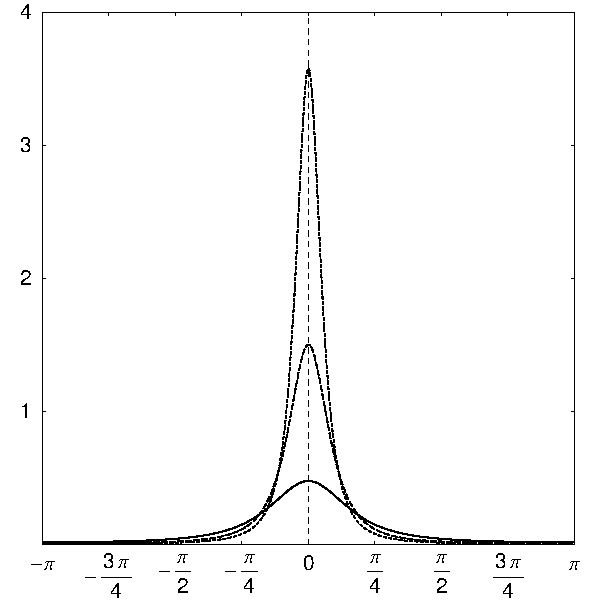
\includegraphics[width=0.7\textwidth]{images/poisson}
  \caption{The Poisson kernel $\fun{Q_{h}}{\cos\theta}$ for $h = 0.5,0.7,0.8$ and $\theta \in \interv{[}{-\pi}{\pi}{]}$.}
  \label{Basics:Figure:PoissonKernel}
\end{figure}

%\begin{figure}[htb]
%  \centering
%   \subfigure[$h=0.70$]
%     {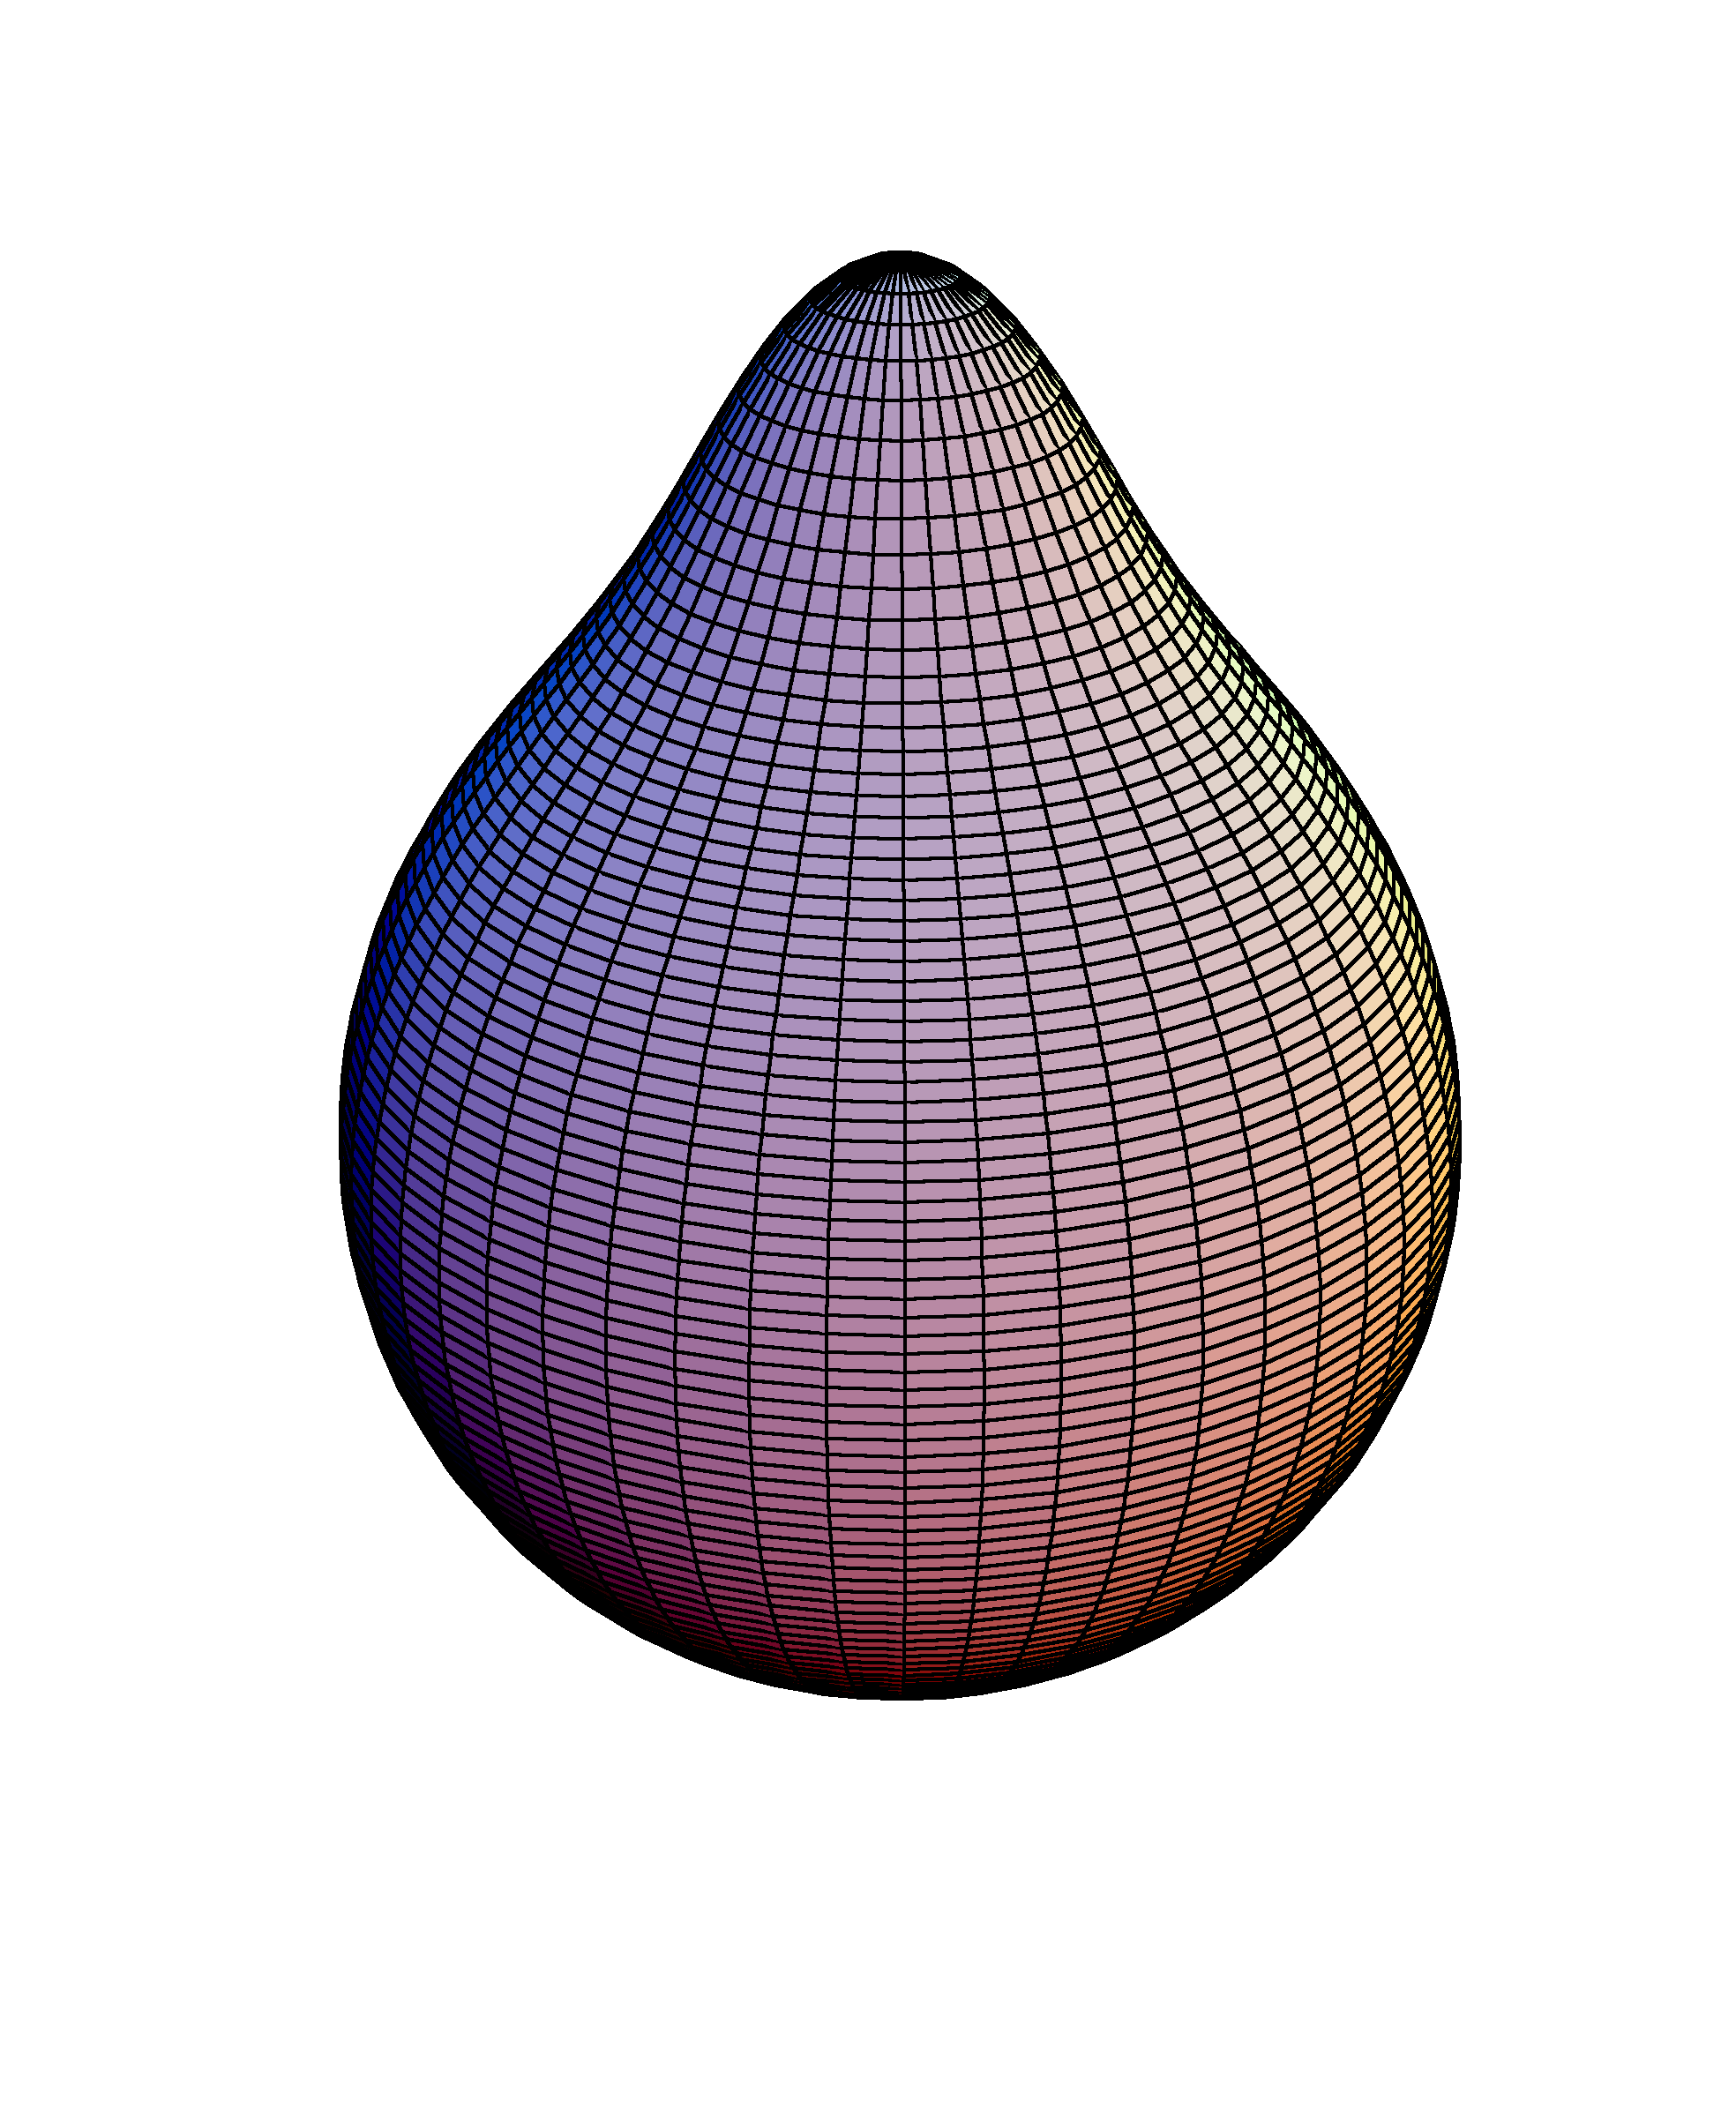
\includegraphics[width=0.5\textwidth]{images/p_070.png}}\hfill
%   \subfigure[$h=0.75$]
%     {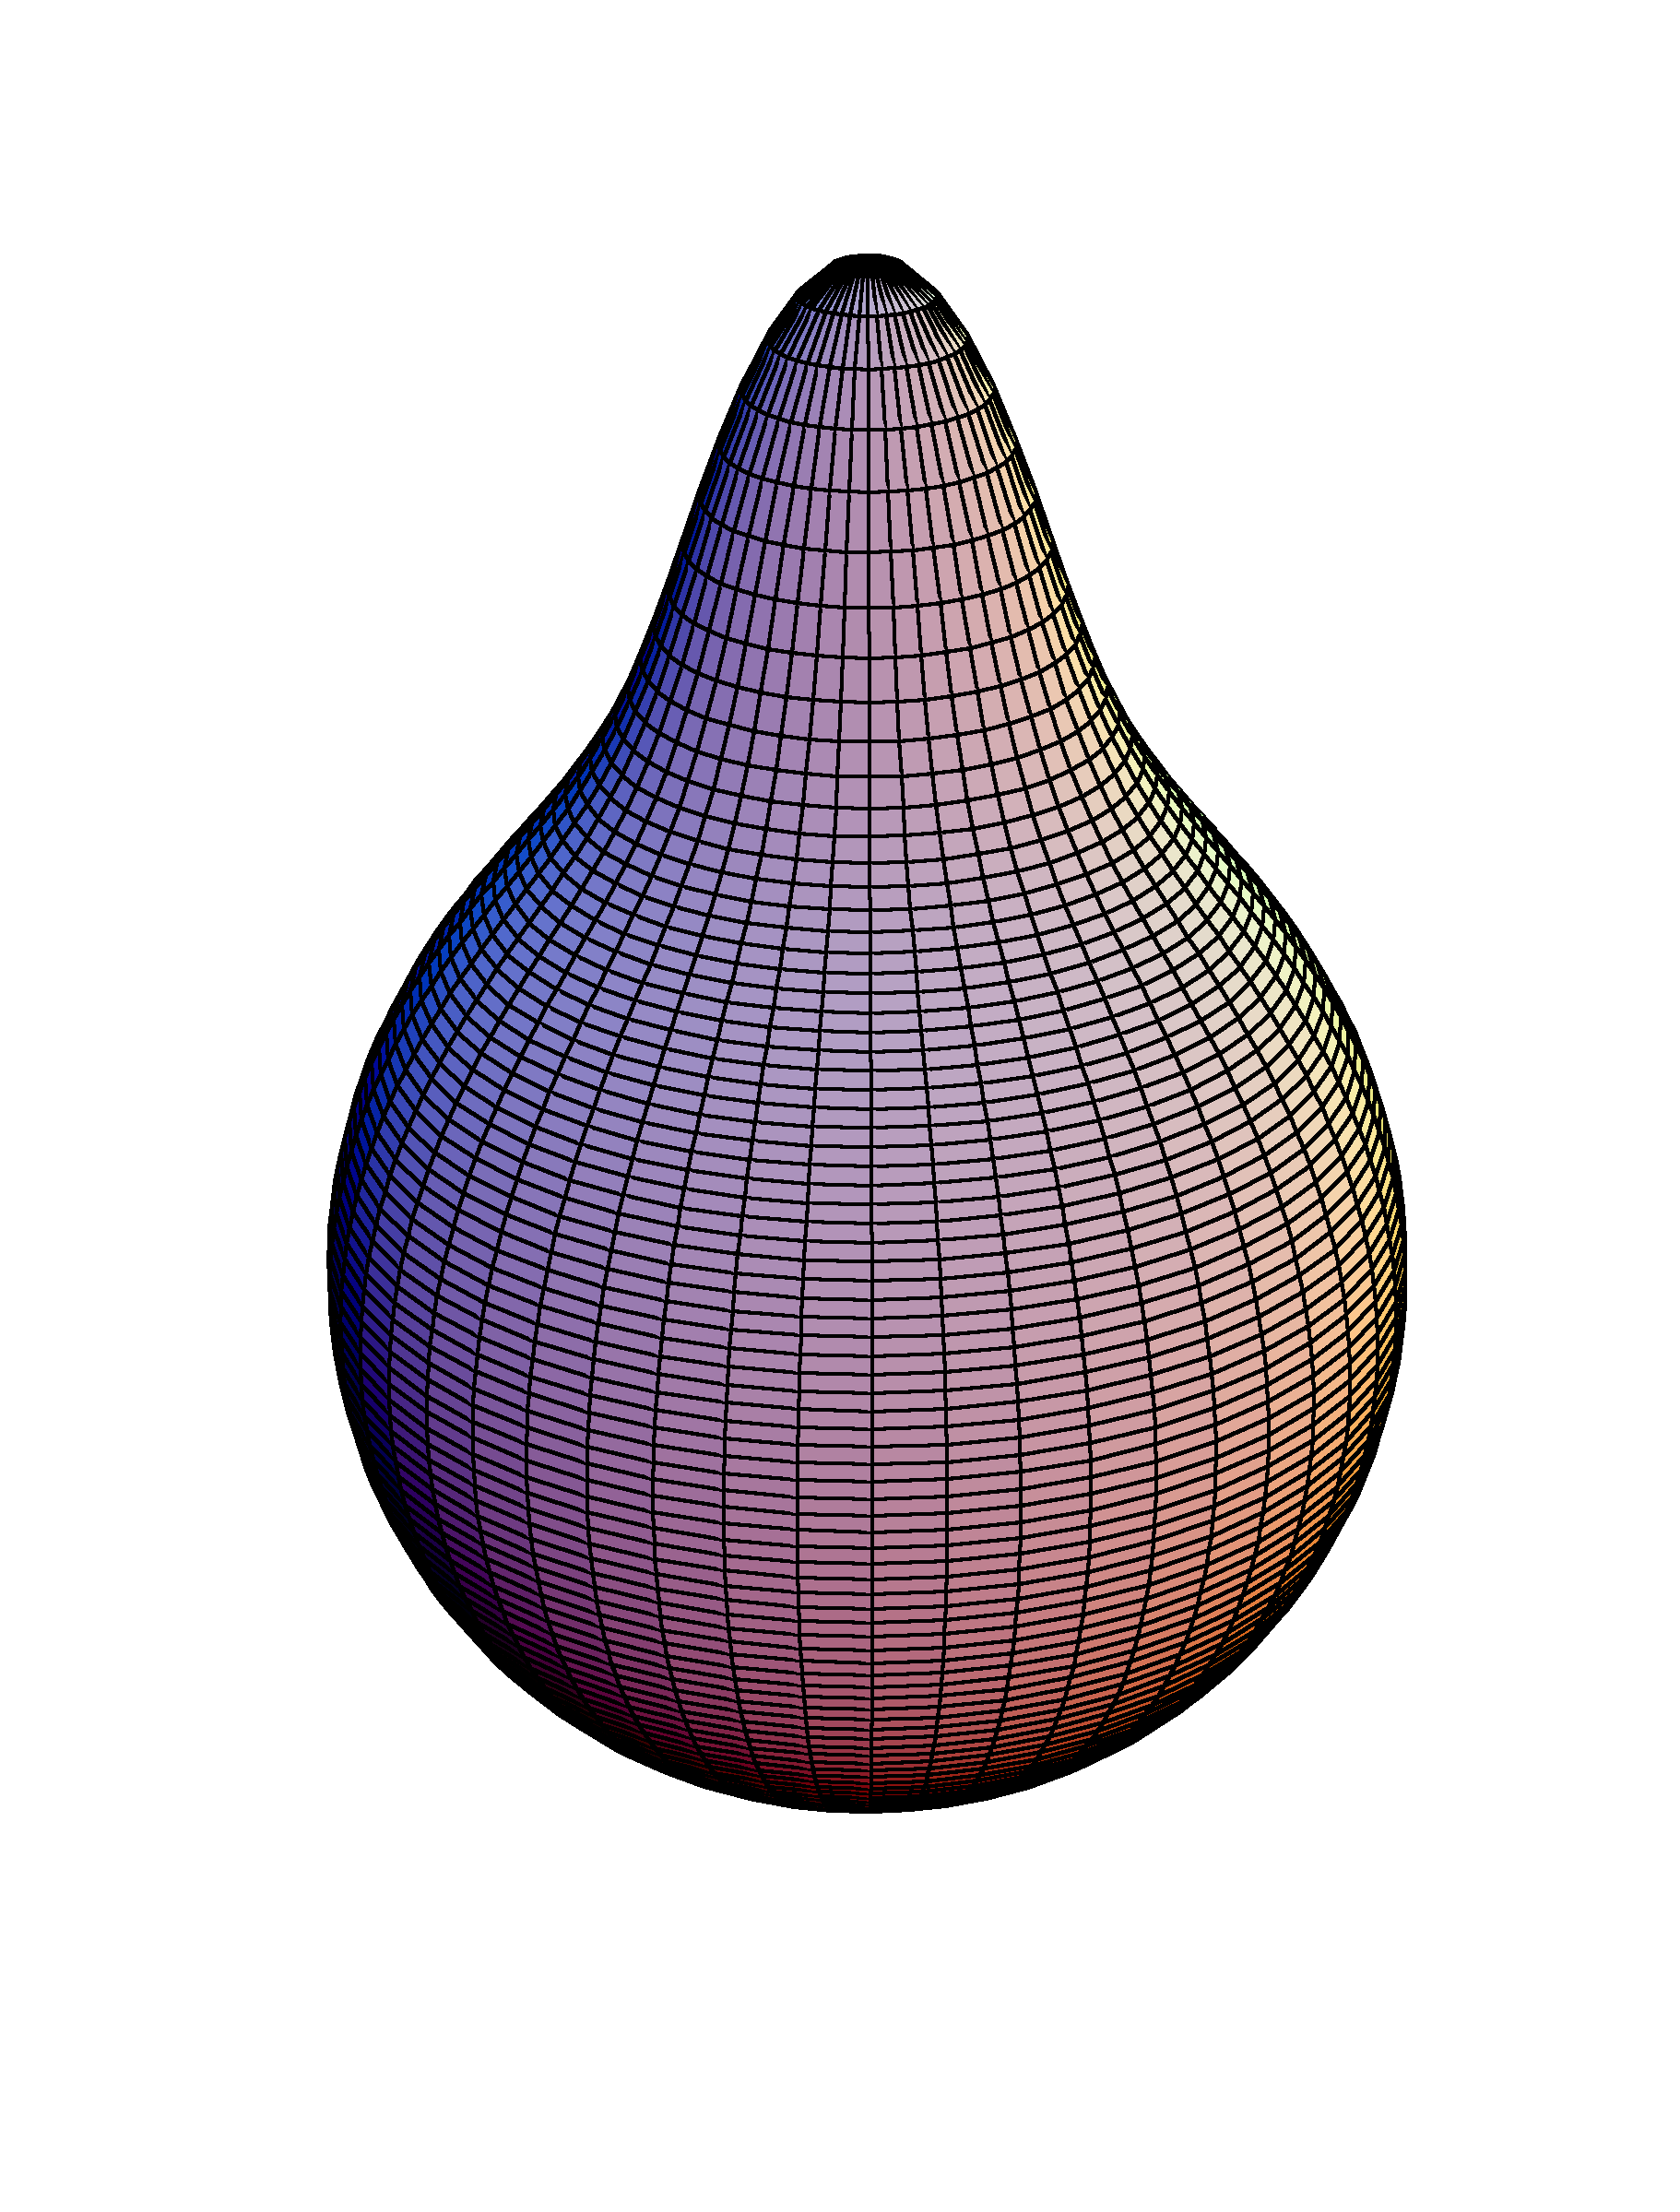
\includegraphics[width=0.5\textwidth]{images/p_075.png}}\\
%   \subfigure[$h=0.80$]
%     {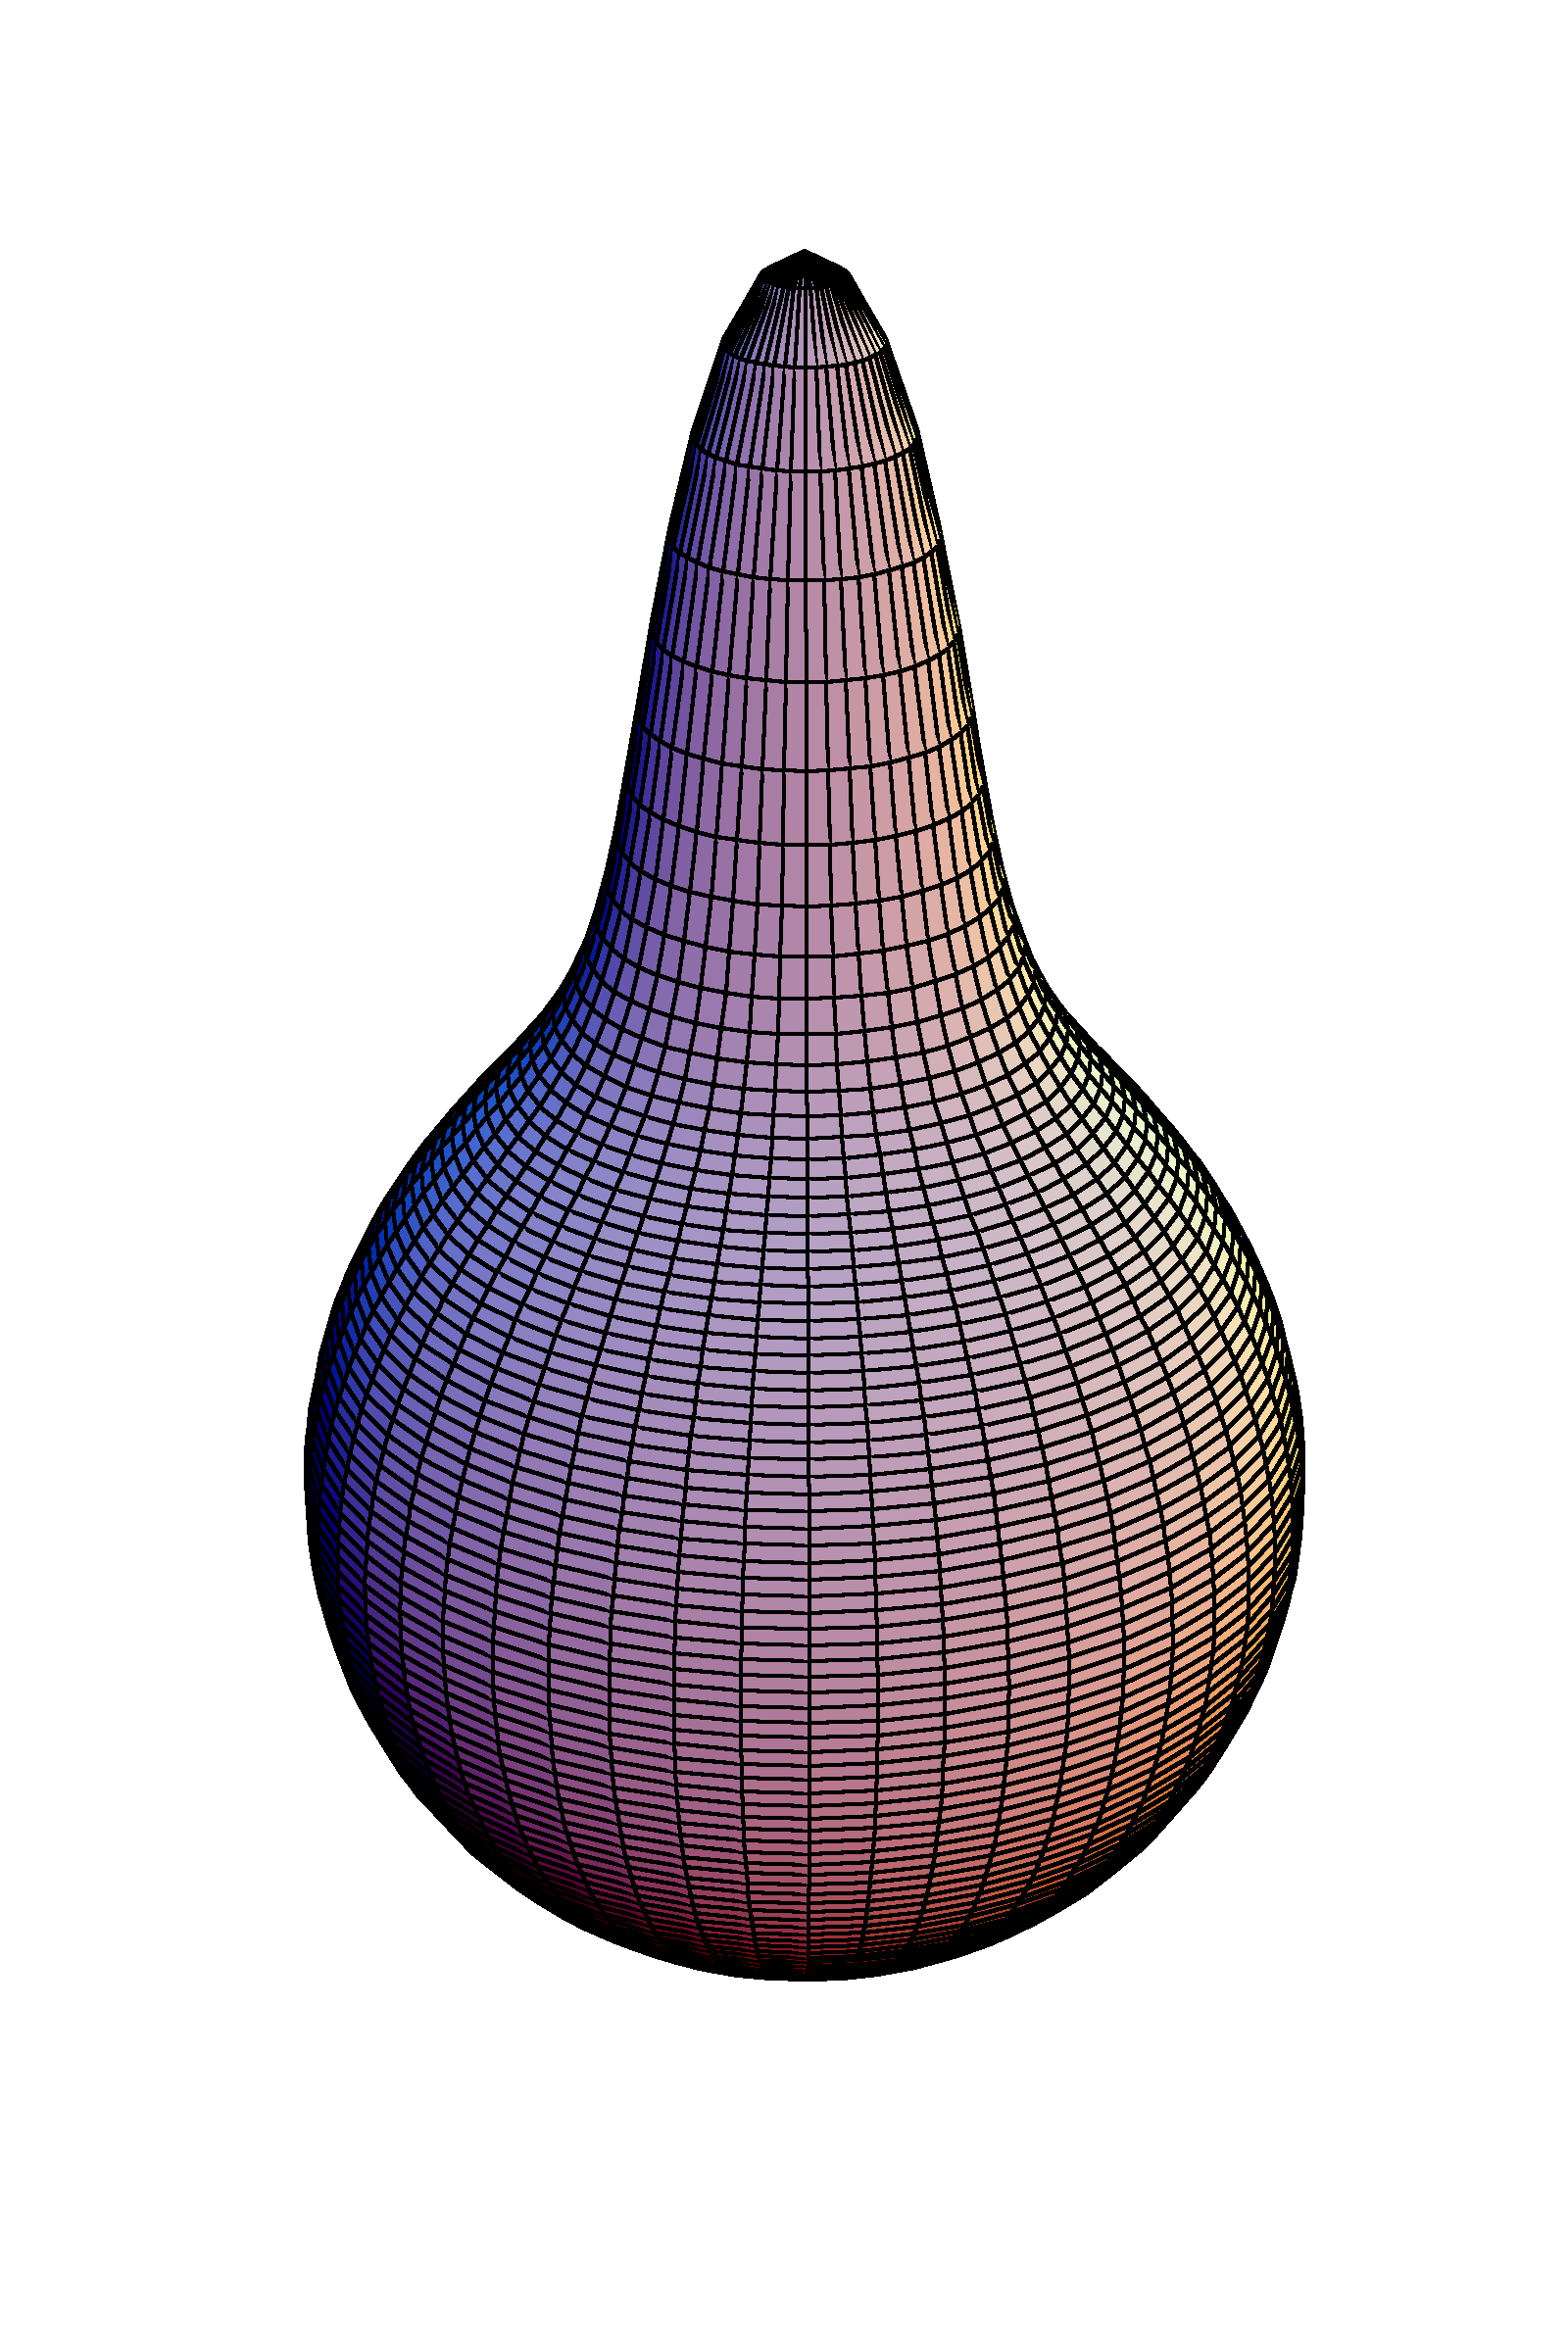
\includegraphics[width=0.5\textwidth]{images/p_080.png}}\hfill
%   \subfigure[$h=0.85$]
%     {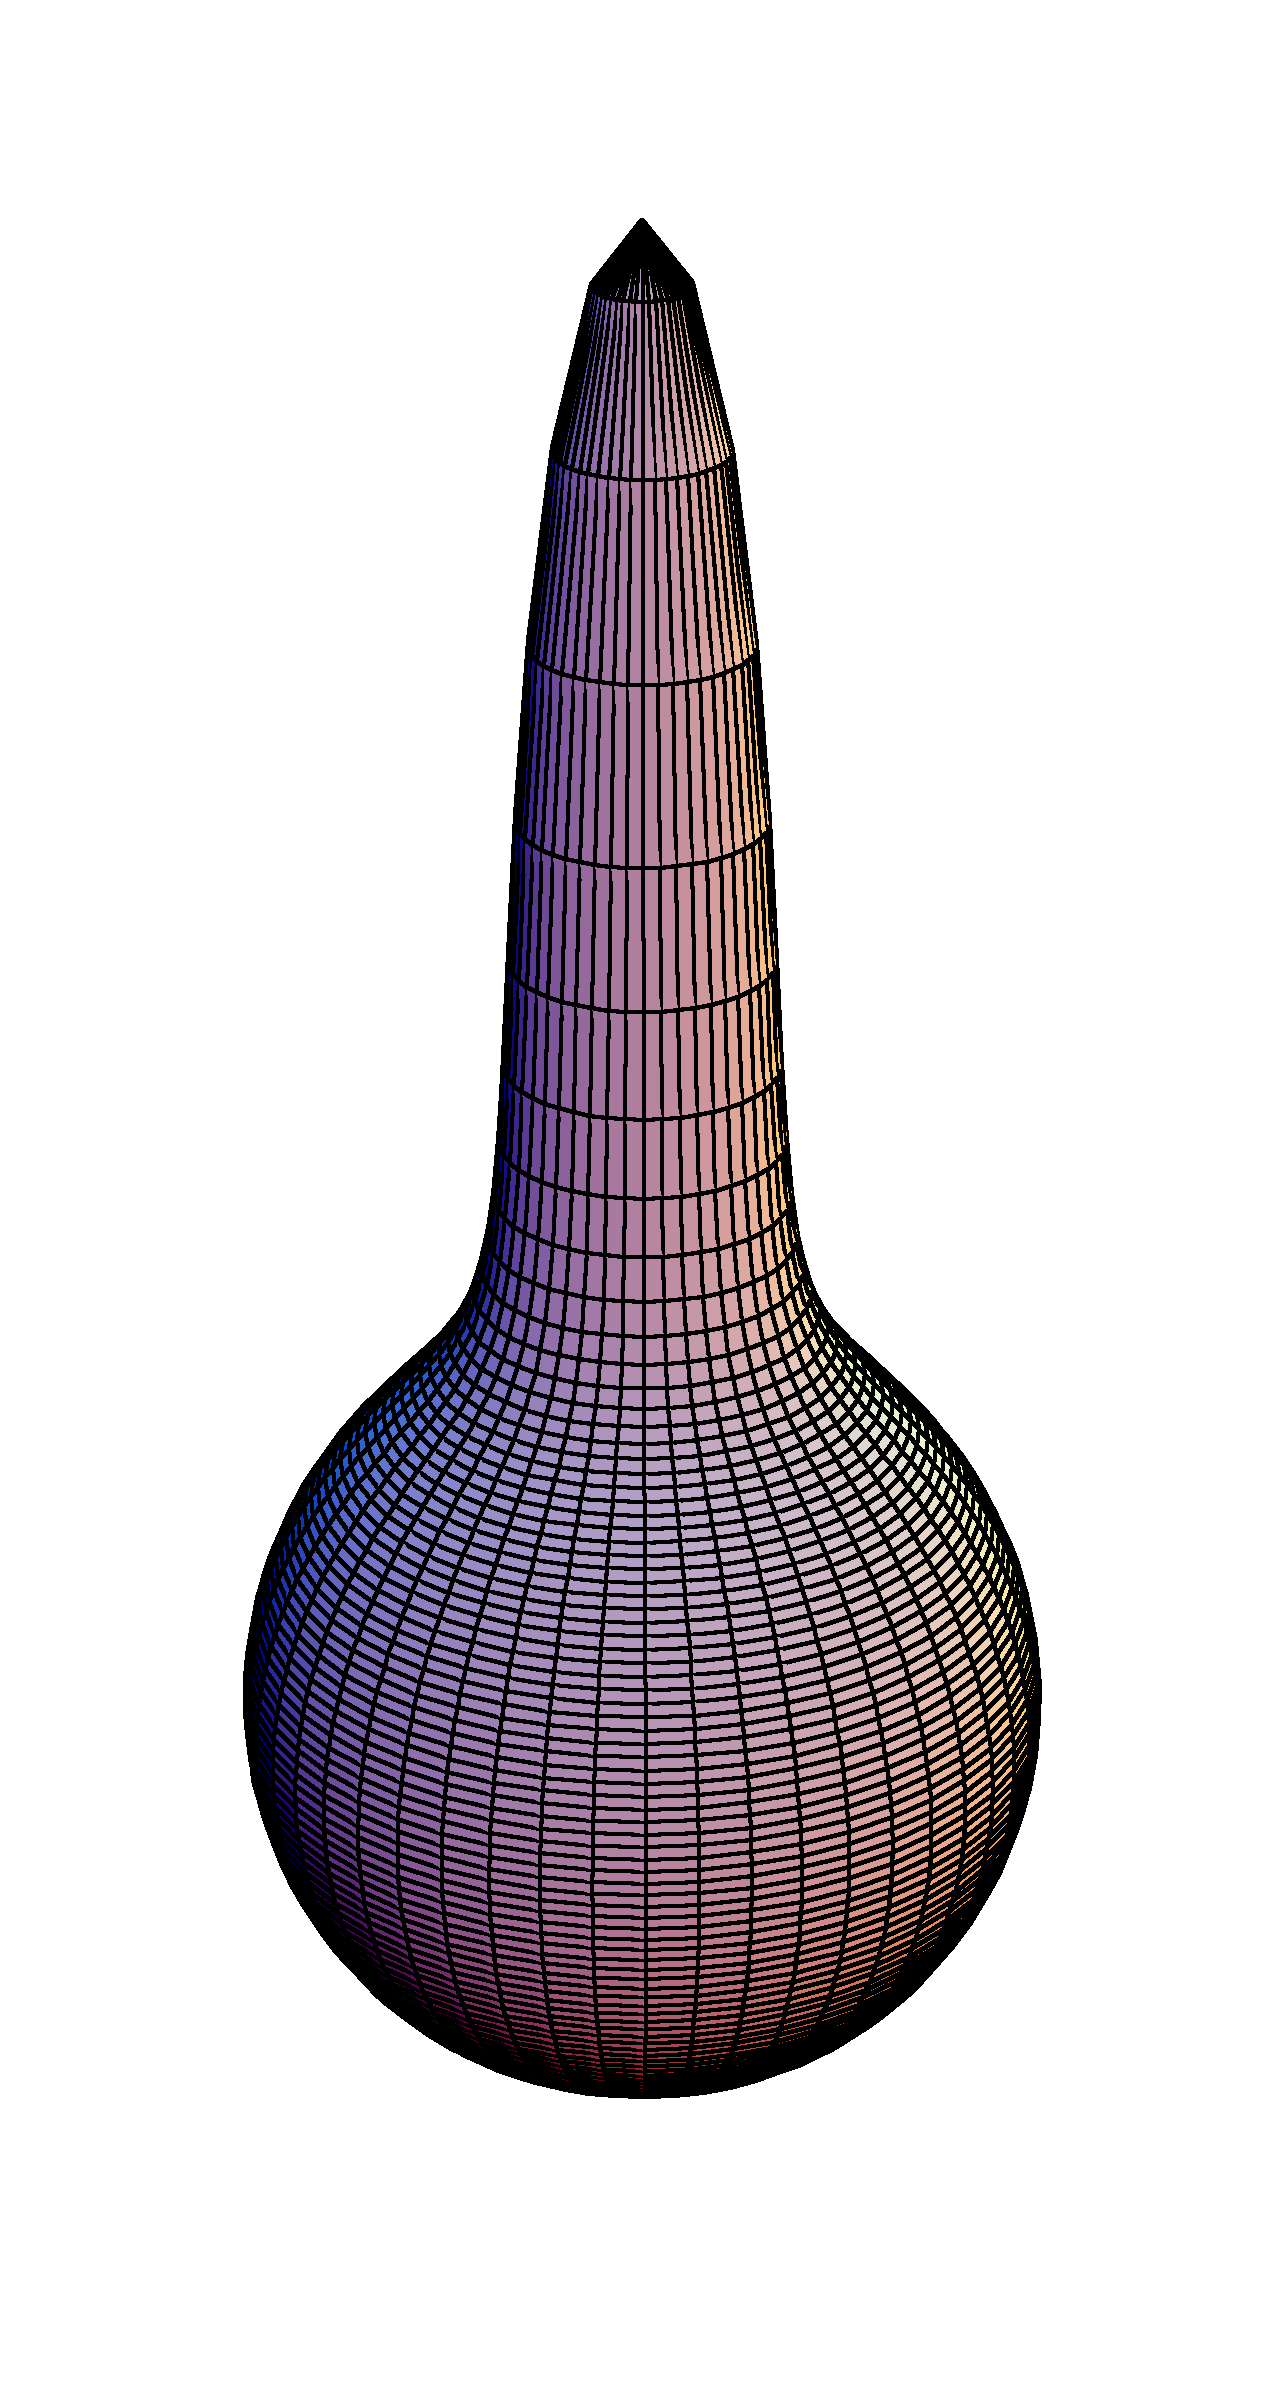
\includegraphics[width=0.5\textwidth]{images/p_085.png}}
%  \caption{The Poisson kernel plotted as a spherical radial basis function on the sphere for different values of $h$.}
%  \label{Basics:Figure:PoissonKernel2}
%\end{figure}

\begin{example}
  We define the \emph{singularity kernel} $S_{h}:\interv{[}{-1}{1}{]} \rightarrow \R$ by
  \[
    \fun{S_{h}}{x} := \frac{1}{2\pi} \frac{1}{\paren{1-2hx+h^2}^{1/2}}  \quad \paren{x \in \interv{[}{-1}{1}{]}}.
  \]
  Using \eqref{Basics:Solution} we obtain
  \[
    \fun{S_{h}}{x} = \sum_{k = 0}^{\infty} \frac{1}{2\pi} h^k \fun{P_k}{x}
  \]
  and therefore
  \[
    \fun{S_{h}^{\wedge}}{k} = \frac{2k+1}{2} h^k.
  \]
  See Figure \ref{Basics:Figure:SingularityKernel} and for more information \cite[pp. 112]{frgesc}.
\end{example}

\begin{figure}[tbp]
  \centering
  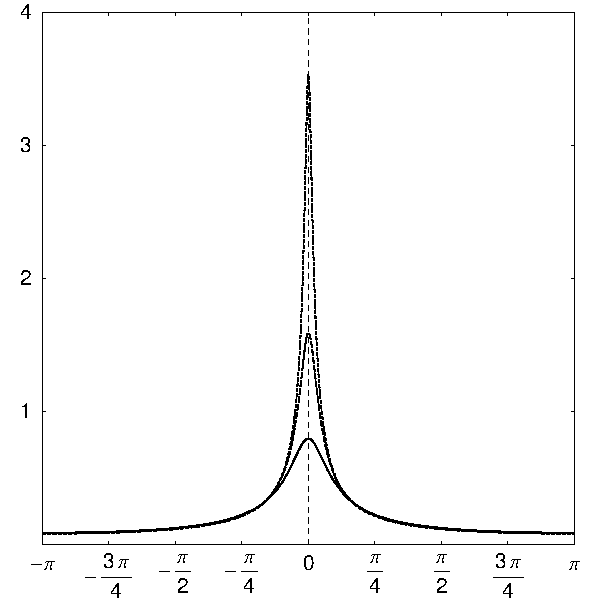
\includegraphics[width=0.7\textwidth]{images/singularity}
  \caption{The singularity kernel $\fun{S_{h}}{\cos\theta}$ for $h = 0.8,0.9,0.95$ and $\theta \in \interv{[}{-\pi}{\pi}{]}$.}
  \label{Basics:Figure:SingularityKernel}
\end{figure}

\begin{example}
  The \emph{Gauss-Weierstra� kernel} $W_{\rho}: \interv{[}{-\pi}{\pi}{]} \rightarrow \R$ is defined by
  \[
    \fun{W_{\rho}}{x} := \sum_{k=0}^{\infty} \e^{-k(k+1)\rho} \frac{2k+1}{4\pi} \fun{P_{k}}{x} \quad \paren{x \in \interv{[}{-1}{1}{]}}.
  \]
  Results due to Bochner (\cite{bochner1950},\cite{bochner1954}) assure $\fun{W_{\rho}}{x} \ge 0$ and we have
  \[
    \int_{\twosphere} \fun{W_{\rho}}{\V{\eta} \cdot \V{\xi}} \dx \V{\xi} = 1.
  \]
  For further properties we refer to \cite{frgesc} again. The kernel function $W_{\rho}$ is illustrated in Figure \ref{Basics:Figure:GaussWeierstrassKernel}.
\end{example}

\begin{figure}[tb]
  \centering
  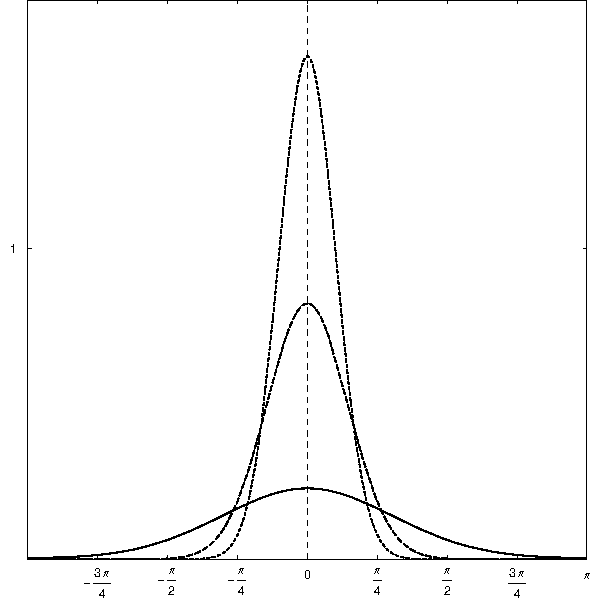
\includegraphics[width=0.7\textwidth]{images/gaussweierstrass}
  \caption{The Gauss-Weierstra� kernel $\fun{W_{\rho}}{\cos\theta}$ for $\rho = 0.4,0.1,0.05$ and $\theta \in \interv{[}{-\pi}{\pi}{]}$.}
  \label{Basics:Figure:GaussWeierstrassKernel}
\end{figure}

\begin{example}
  The locally supported kernel $L_{h,\lambda}: \interv{[}{-1}{1}{]} \rightarrow \R$ mentioned in \cite{frsc} and defined by
  \[
    \fun{L_{h,\lambda}}{x} := 
      \left\{\begin{array}{l@{\quad \text{if} \quad}l} 
                                              0 & -1 \le x \le h, \\
        \frac{\lambda+1}{2\pi(1-h)^{\lambda+1}}\paren{x-h}^{\lambda} &  h   < x \le 1,
      \end{array}\right.
  \]
  has the recursively defined symbol $\fun{L_{h,\lambda}^{\wedge}}{k}$ with
\begin{eqnarray*}
    \fun{L_{h,\lambda}^{\wedge}}{0} & = & 1,\\
    \paren{\lambda+1} \fun{L_{h,\lambda}^{\wedge}}{1} & = & \paren{\lambda + 1 + h},\\
    \paren{k+\lambda+2} \fun{L_{h,\lambda}^{\wedge}}{k+1} & = & \paren{2k+1} h \fun{L_{h,\lambda}^{\wedge}}{k} - \paren{k-\lambda-1} \fun{L_{h,\lambda}^{\wedge}}{k-1} 
    \quad \paren{k = 1,2,\ldots}.
\end{eqnarray*}
  Figure \ref{Basics:Figure:LKernel} shows the function $L_{h,\lambda}$ for different values $h$ and $\lambda$.
\end{example}

\begin{figure}[tb]
  \centering
   \subfigure[$\lambda=1.5$]
     {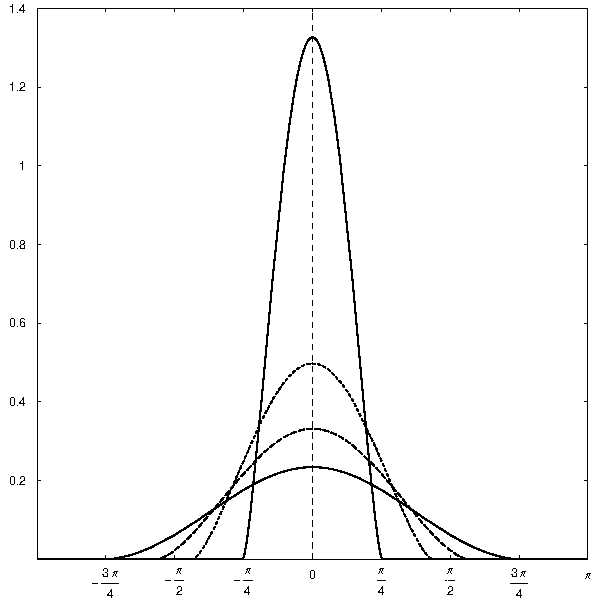
\includegraphics[width=0.33\textwidth]{images/locsup4}}\hfill
   \subfigure[$\lambda=1.0$]
     {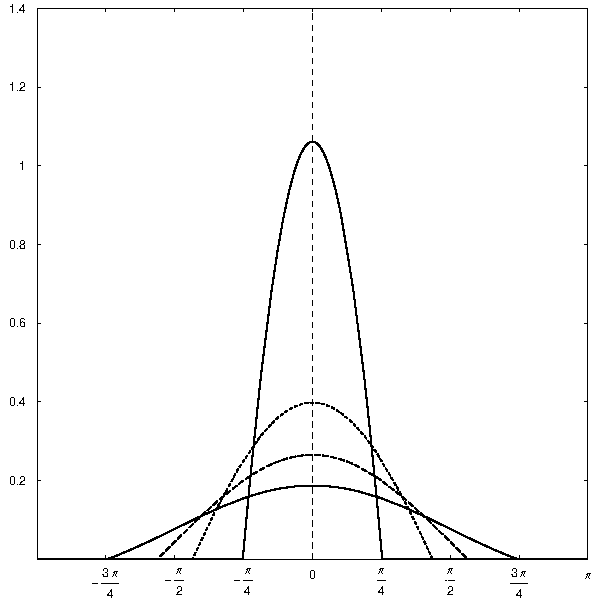
\includegraphics[width=0.33\textwidth]{images/locsup3}}\\
   \subfigure[$\lambda=0.5$]
     {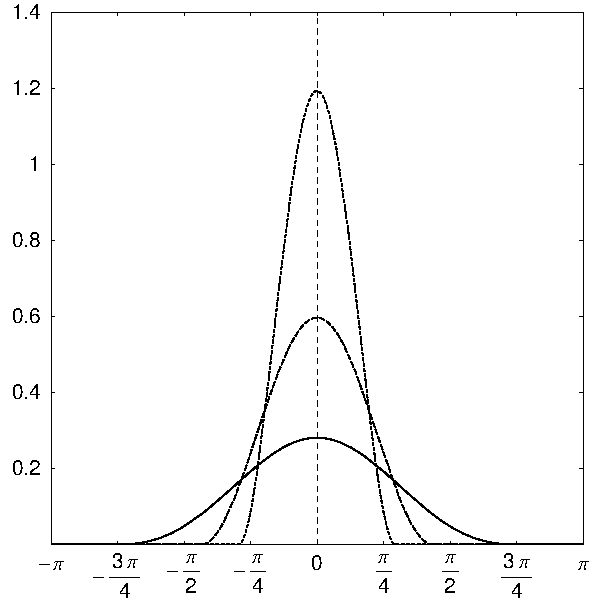
\includegraphics[width=0.33\textwidth]{images/locsup2}}\hfill
   \subfigure[$\lambda=0.2$]
     {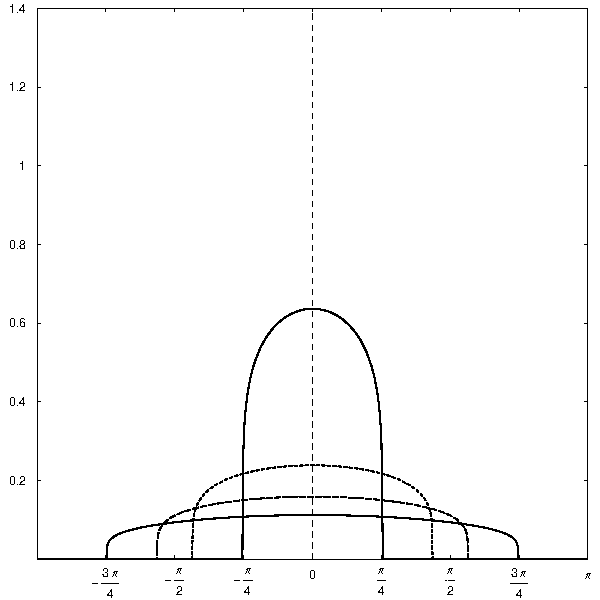
\includegraphics[width=0.33\textwidth]{images/locsup1}}
  \caption{The kernel $L_{h,\lambda}$ for $h = -0.7, -0.2, 0.2, 0.7$ and different values of $\lambda$.}
  \label{Basics:Figure:LKernel}
\end{figure}
\section{Spherical Radial Basis Functions}
\label{Basics:SphericalKernels}

\emph{Spherical radial basis basis functions} are the spherical counterpart of radial basis functions in Euclidean spaces. 
Generally, one starts with a function $K$ from $\Ln{2}{\interv{[}{-1}{1}{]}}$
%$: \interv{[}{-1}{1}{]} \rightarrow \C$ 
and defines for fixed $\V{\eta} \in \twosphere$ the $\V{\eta}$-zonal function 
\[
  \fun{K}{\V{\eta} \: \cdot}: \twosphere \rightarrow \C,\ \V{\xi} \mapsto \fun{K}{\V{\eta} \cdot \V{\xi}} \quad \paren{\V{\xi} \in \twosphere}.\] 
%by \[ \fun{K_{\V{\eta}}}{\V{\xi}} := \fun{G}{\V{\eta} \cdot \V{\xi}}.\]
By means of the \emph{Funk-Hecke formula} (see \cite[pp. 60]{frgesc}) we obtain for fixed $k \in \NZ$
\[
  \scalarproduct{\fun{K}{\V{\eta} \: \cdot}}{Y_{k}^n} = \int_{\twosphere} \fun{K}{\V{\eta} \cdot \V{\xi}} \overline{\fun{Y_{k}^n}{\V{\xi}}} \: \dx \V{\xi} = \fun{K^{\wedge}}{k} \overline{\fun{Y_{k}^n}{\V{\eta}}} \quad \paren{n=-k,\ldots,k},
\]
where the \emph{Legendre transform}, i.e. the \emph{symbol} of $K$, is given by
\[
  \fun{K^{\wedge}}{k} := 2 \pi \int_{-1}^{1} \fun{K}{x} \fun{P_{k}}{x} \dx x \quad \paren{k \in \NZ}.
\]
%We refer the interested reader to \cite{} and \cite{} for more details.
%The function $G$ can be developed into a series of Legendre polynomials
%\[ \fun{G}{x} = \sum_{k = 0}^{\infty} a_k \fun{P_k}{x}.\]
%where the coefficients $a_k$ are the scalar products
%\[ a_k = \scalarproduct{G}{P_{k}}_{\interv{[}{-1}{1}{]}} = \int_{-1}^{1} \fun{G}{x} \fun{P_k}{x} \dx x.\]
We have therefore 
\begin{equation}
  \label{Basics:Kernel}
  \fun{K}{\V{\eta} \cdot \V{\xi}} = \sum_{k = 0}^{\infty} \sum_{n=-k}^k \fun{K^{\wedge}}{k} \overline{\fun{Y_{k}^n}{\V{\eta}}} \fun{Y_{k}^n}{\V{\xi}} 
\end{equation}
and applying the Addition Theorem from Proposition \ref{Basics:AdditionTheorem}, we obtain for $K$ the orthogonal expansion
\begin{equation}
\label{Basics:OrthogonalKernelExpansion}
  \fun{K}{x} = \sum_{k = 0}^{\infty} \frac{2k+1}{4\pi} \fun{K^{\wedge}}{k} \fun{P_k}{x} \quad \paren{x \in \interv{[}{-1}{1}{]}}.
\end{equation}
%One is often interested in evaluating such an expansion on the sphere in a fast way when dealing with 
%spherical convolution. As an application of the algorithms developed in this text, one can derive 
%an algorithm based on the discrete spherical Fourier transform, as shown in Chapter \ref{}.

\begin{example}
We consider the generating series
\begin{equation}
  \label{Basics:GeneratingFunction}
  \fun{\phi}{h} := \sum_{k = 0}^{\infty} h^k \fun{P_k}{x} \quad \paren{x \in \interv{[}{-1}{1}{]}}
\end{equation}
which is absolutely and uniformly convergent for $h \in
\interv{(}{-1}{1}{)}$ with
\begin{equation}
  \label{Basics:Solution}
  \sum_{k = 0}^{\infty} h^k \fun{P_k}{x} = \frac{1}{\sqrt{1-2hx+h^2}}.
\end{equation}
This follows from the ordinary differential equation
\begin{equation}
\label{Basics:DifferentialEquation}
  \paren{1+h^2-2hx}\fun{\phi'}{h} = \paren{x-h}\fun{\phi}{h}
\end{equation}
obtained by differentiation with respect to $h$ and comparing coefficients in line with \eqref{Basics:GeneratingFunction}. Using the initial 
condition $\fun{\phi}{0}=1$ this yields the unique solution \eqref{Basics:Solution} of \eqref{Basics:DifferentialEquation}.
From this result, the identity
\begin{equation}
  \nonumber
  \sum_{k=0}^{\infty} \paren{2k+1} h^k \fun{P_k}{x} =
  \frac{1-h^2}{\paren{1-2hx+h^2}^{3/2}}
\end{equation}
 follows easily. When $h$ is restricted to $\interv{(}{0}{1}{)}$ the function
$Q_{h}:\interv{[}{-1}{1}{]} \rightarrow \R$, with
\begin{equation}
  \label{PoissonKernel}
  \nonumber
  \fun{Q_{h}}{x} := \frac{1}{4\pi} \frac{1-h^2}{\paren{1-2hx+h^2}^{3/2}} \quad \paren{x \in \interv{[}{-1}{1}{]}},
\end{equation}
is called \emph{Poisson kernel}. The symbol $\fun{Q_{h}^{\wedge}}{k}$ is given by 
\[
  \fun{Q_{h}^{\wedge}}{k} = h^k.
\]
We refer to Figure \ref{Basics:Figure:PoissonKernel} 
%and \ref{Basics:Figure:PoissonKernel2}
for a visual impression and mention that the parameter $h$
allows for controlling the concentration of the function's energy around
$x = 1$. The Poisson kernel is a positive function and normalized with
\[
  \int_{\twosphere} \fun{Q_{h}}{\V{\eta} \cdot \V{\xi}} \dx \V{\xi} = 1 \quad \paren{\V{\eta} \in \twosphere}.
\]
Further properties with respect to localization and smoothness are derived in \cite[pp. 112]{frgesc}.
\end{example}

\begin{figure}[tbp]
  \centering
  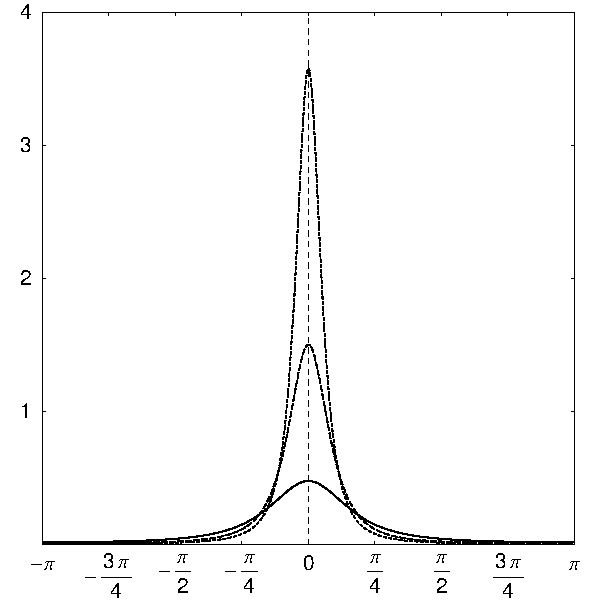
\includegraphics[width=0.7\textwidth]{images/poisson}
  \caption{The Poisson kernel $\fun{Q_{h}}{\cos\theta}$ for $h = 0.5,0.7,0.8$ and $\theta \in \interv{[}{-\pi}{\pi}{]}$.}
  \label{Basics:Figure:PoissonKernel}
\end{figure}

%\begin{figure}[htb]
%  \centering
%   \subfigure[$h=0.70$]
%     {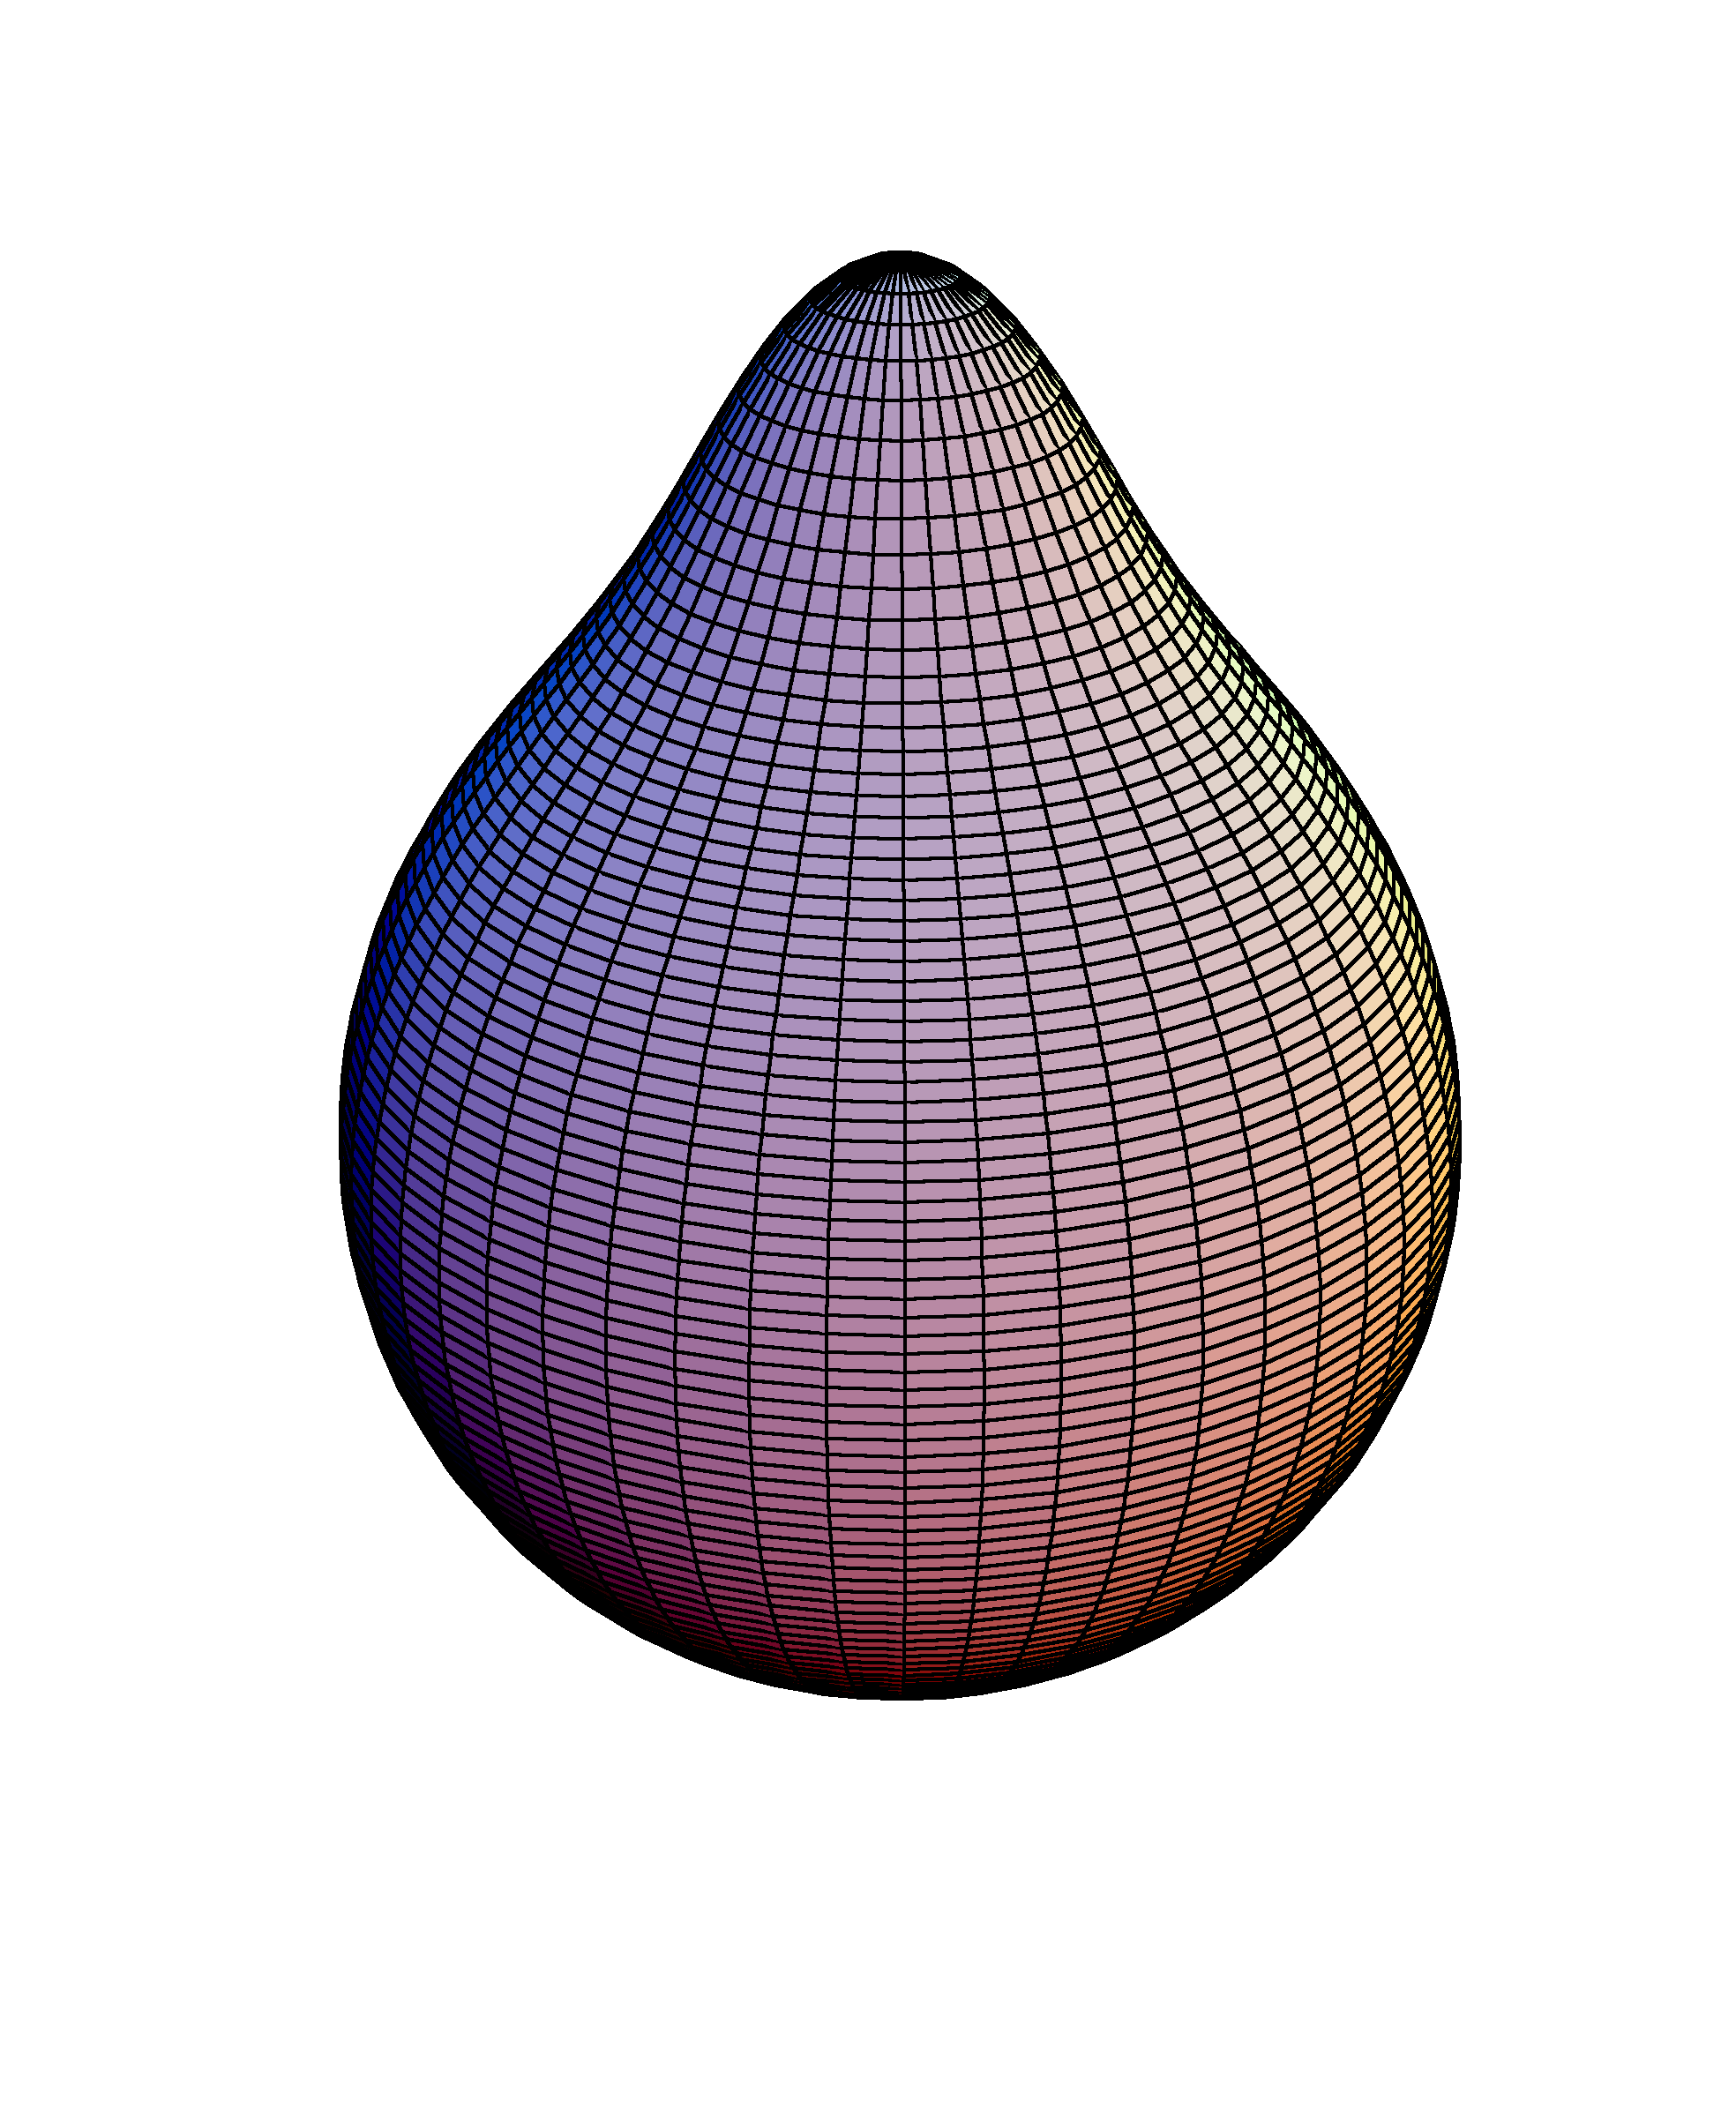
\includegraphics[width=0.5\textwidth]{images/p_070.png}}\hfill
%   \subfigure[$h=0.75$]
%     {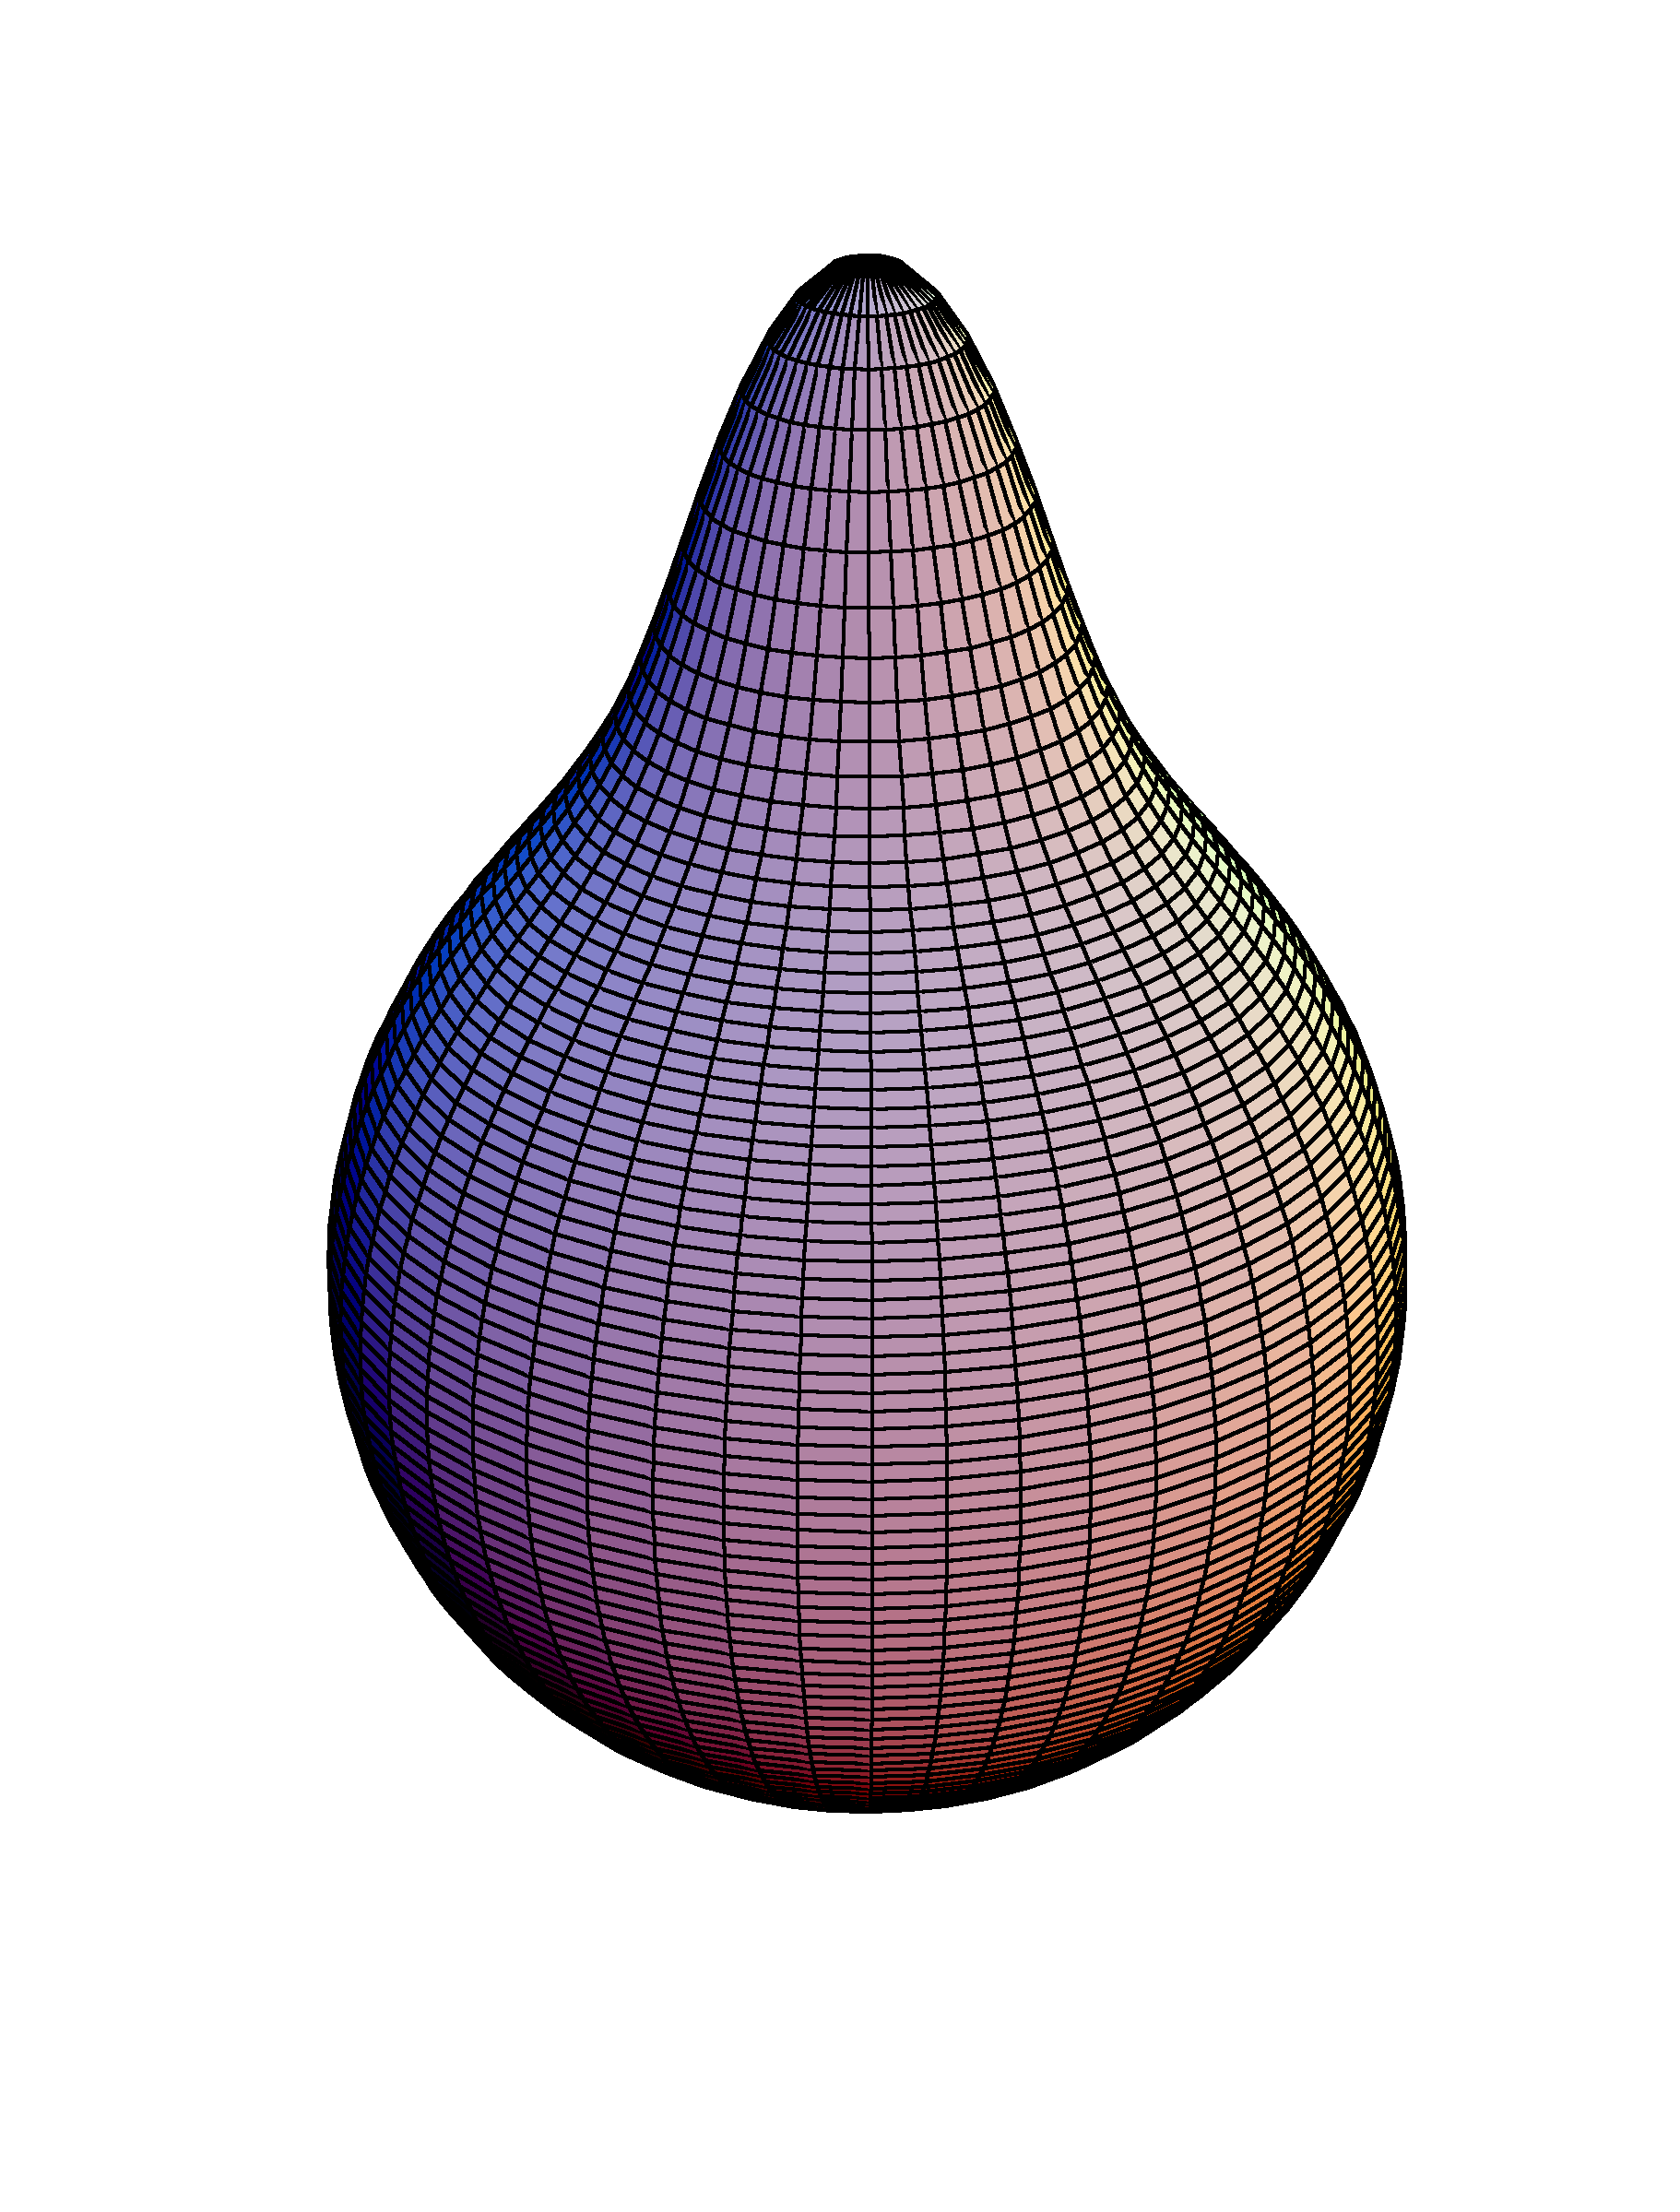
\includegraphics[width=0.5\textwidth]{images/p_075.png}}\\
%   \subfigure[$h=0.80$]
%     {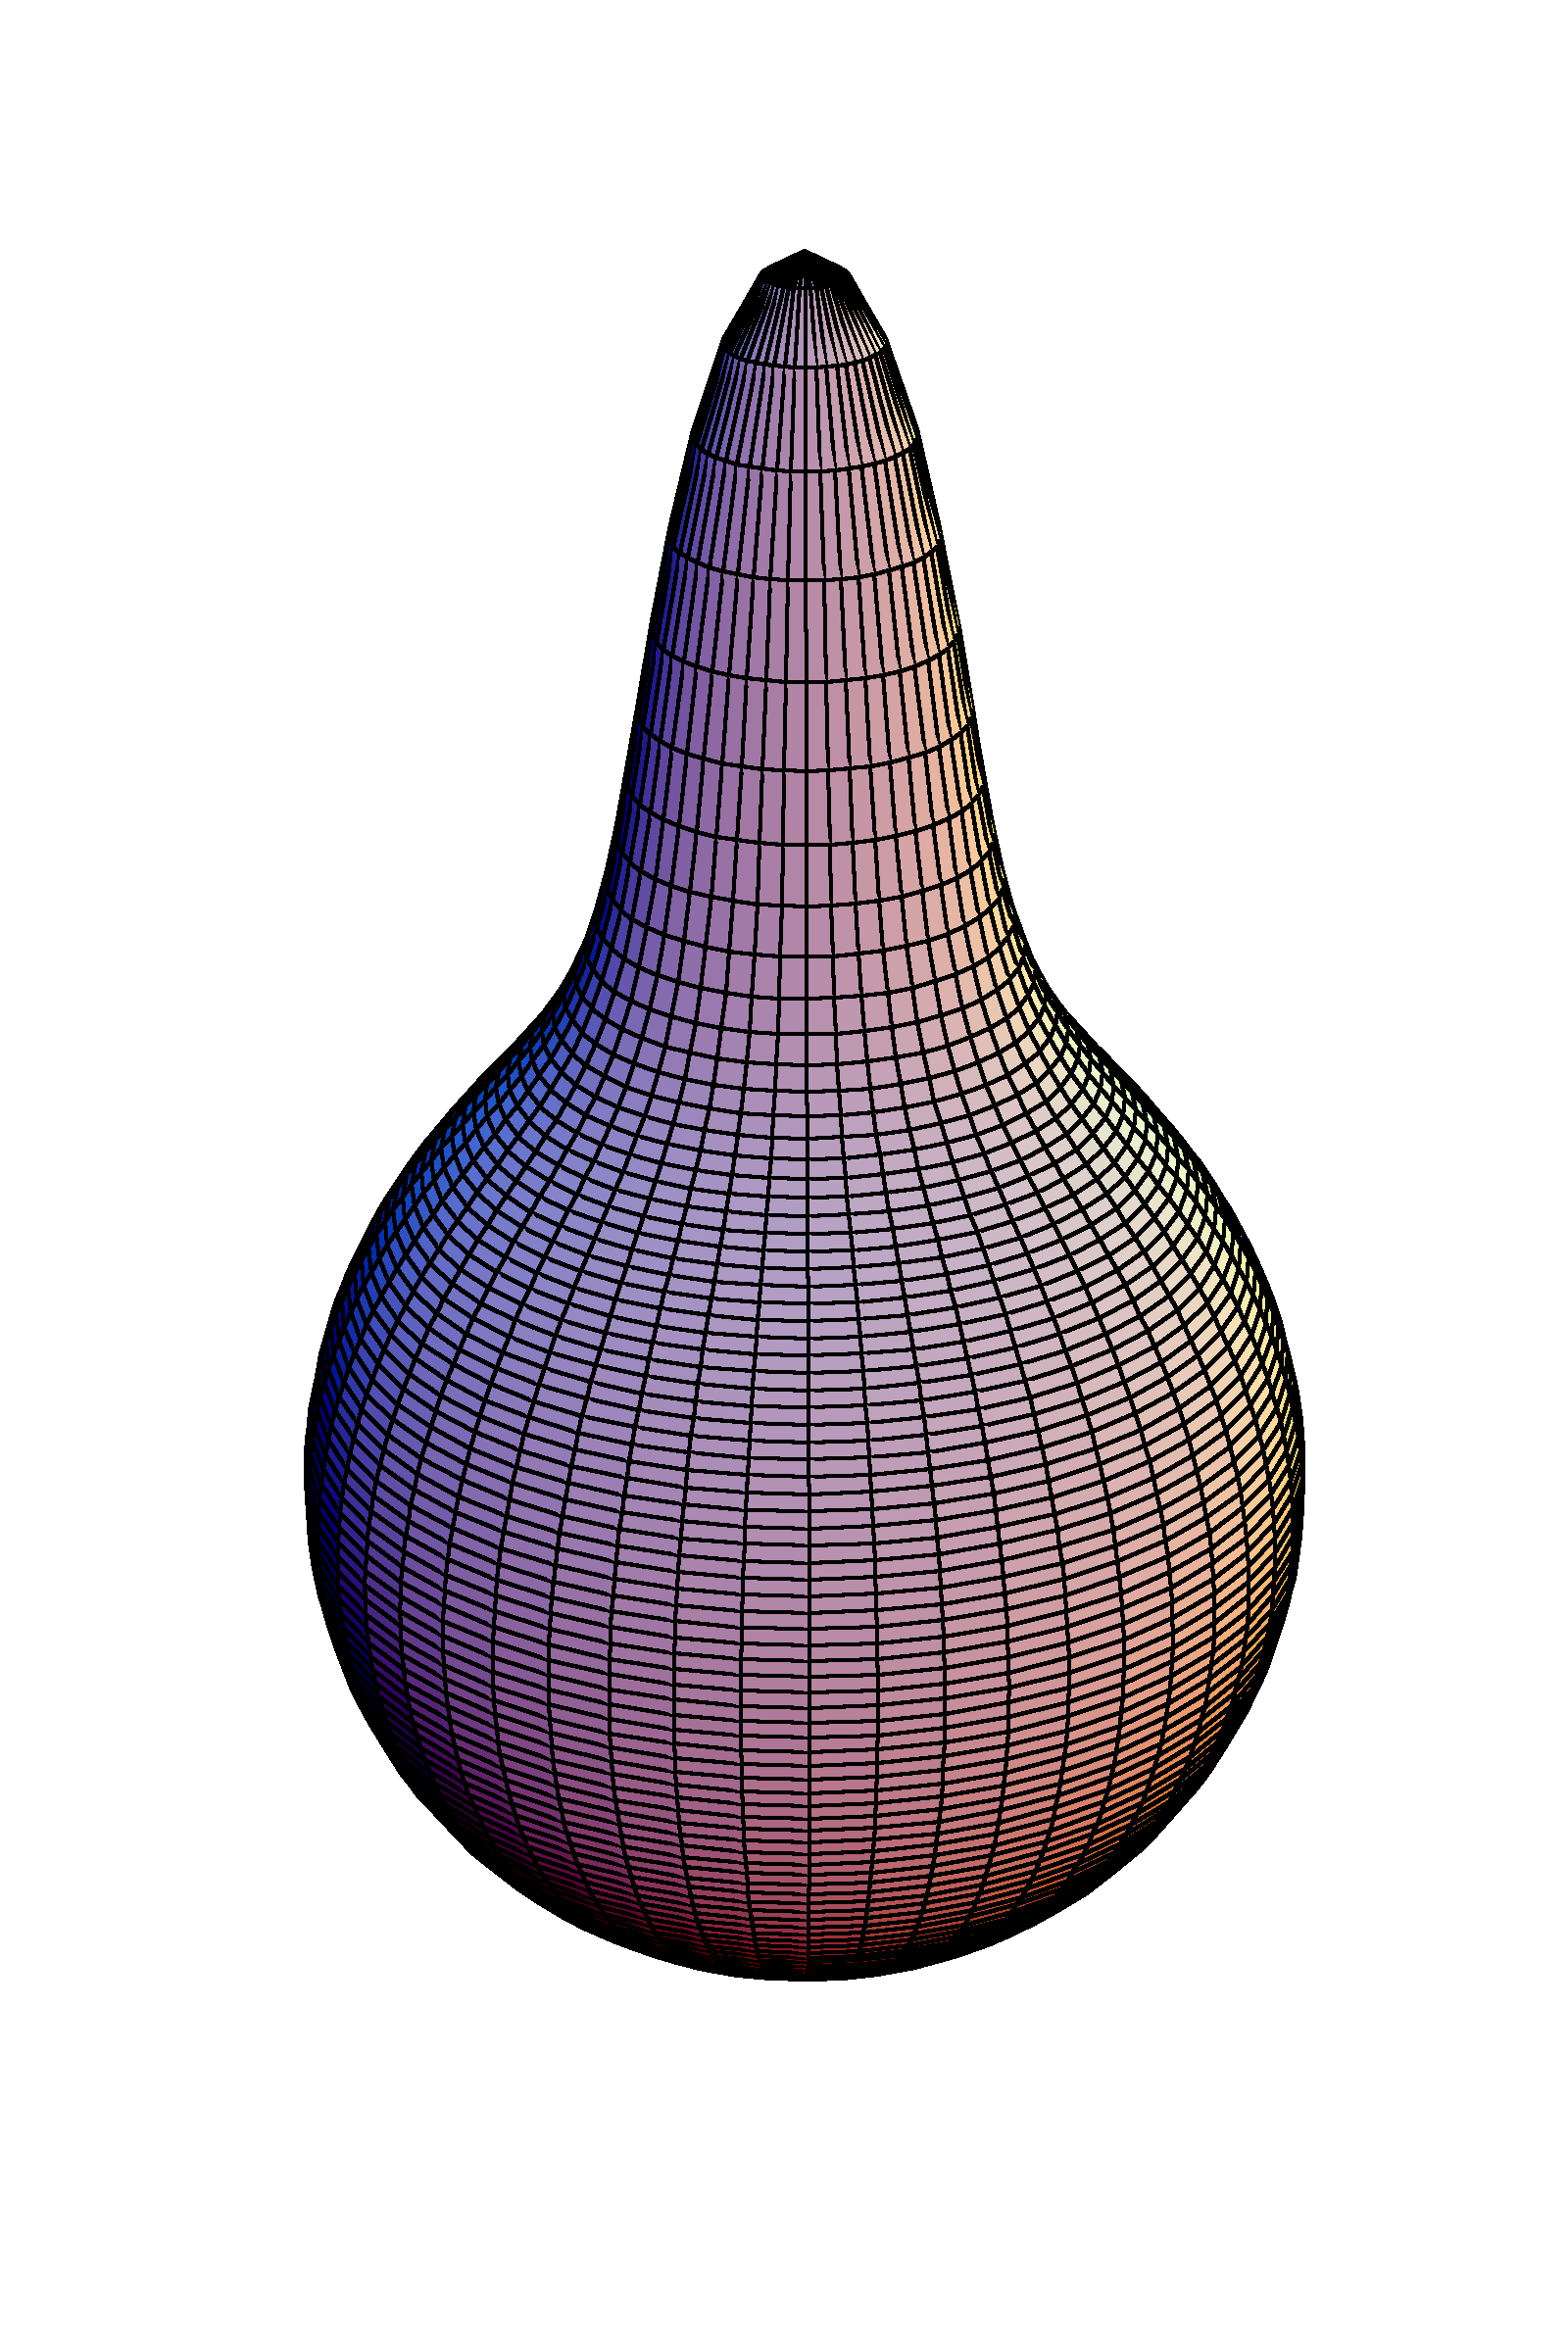
\includegraphics[width=0.5\textwidth]{images/p_080.png}}\hfill
%   \subfigure[$h=0.85$]
%     {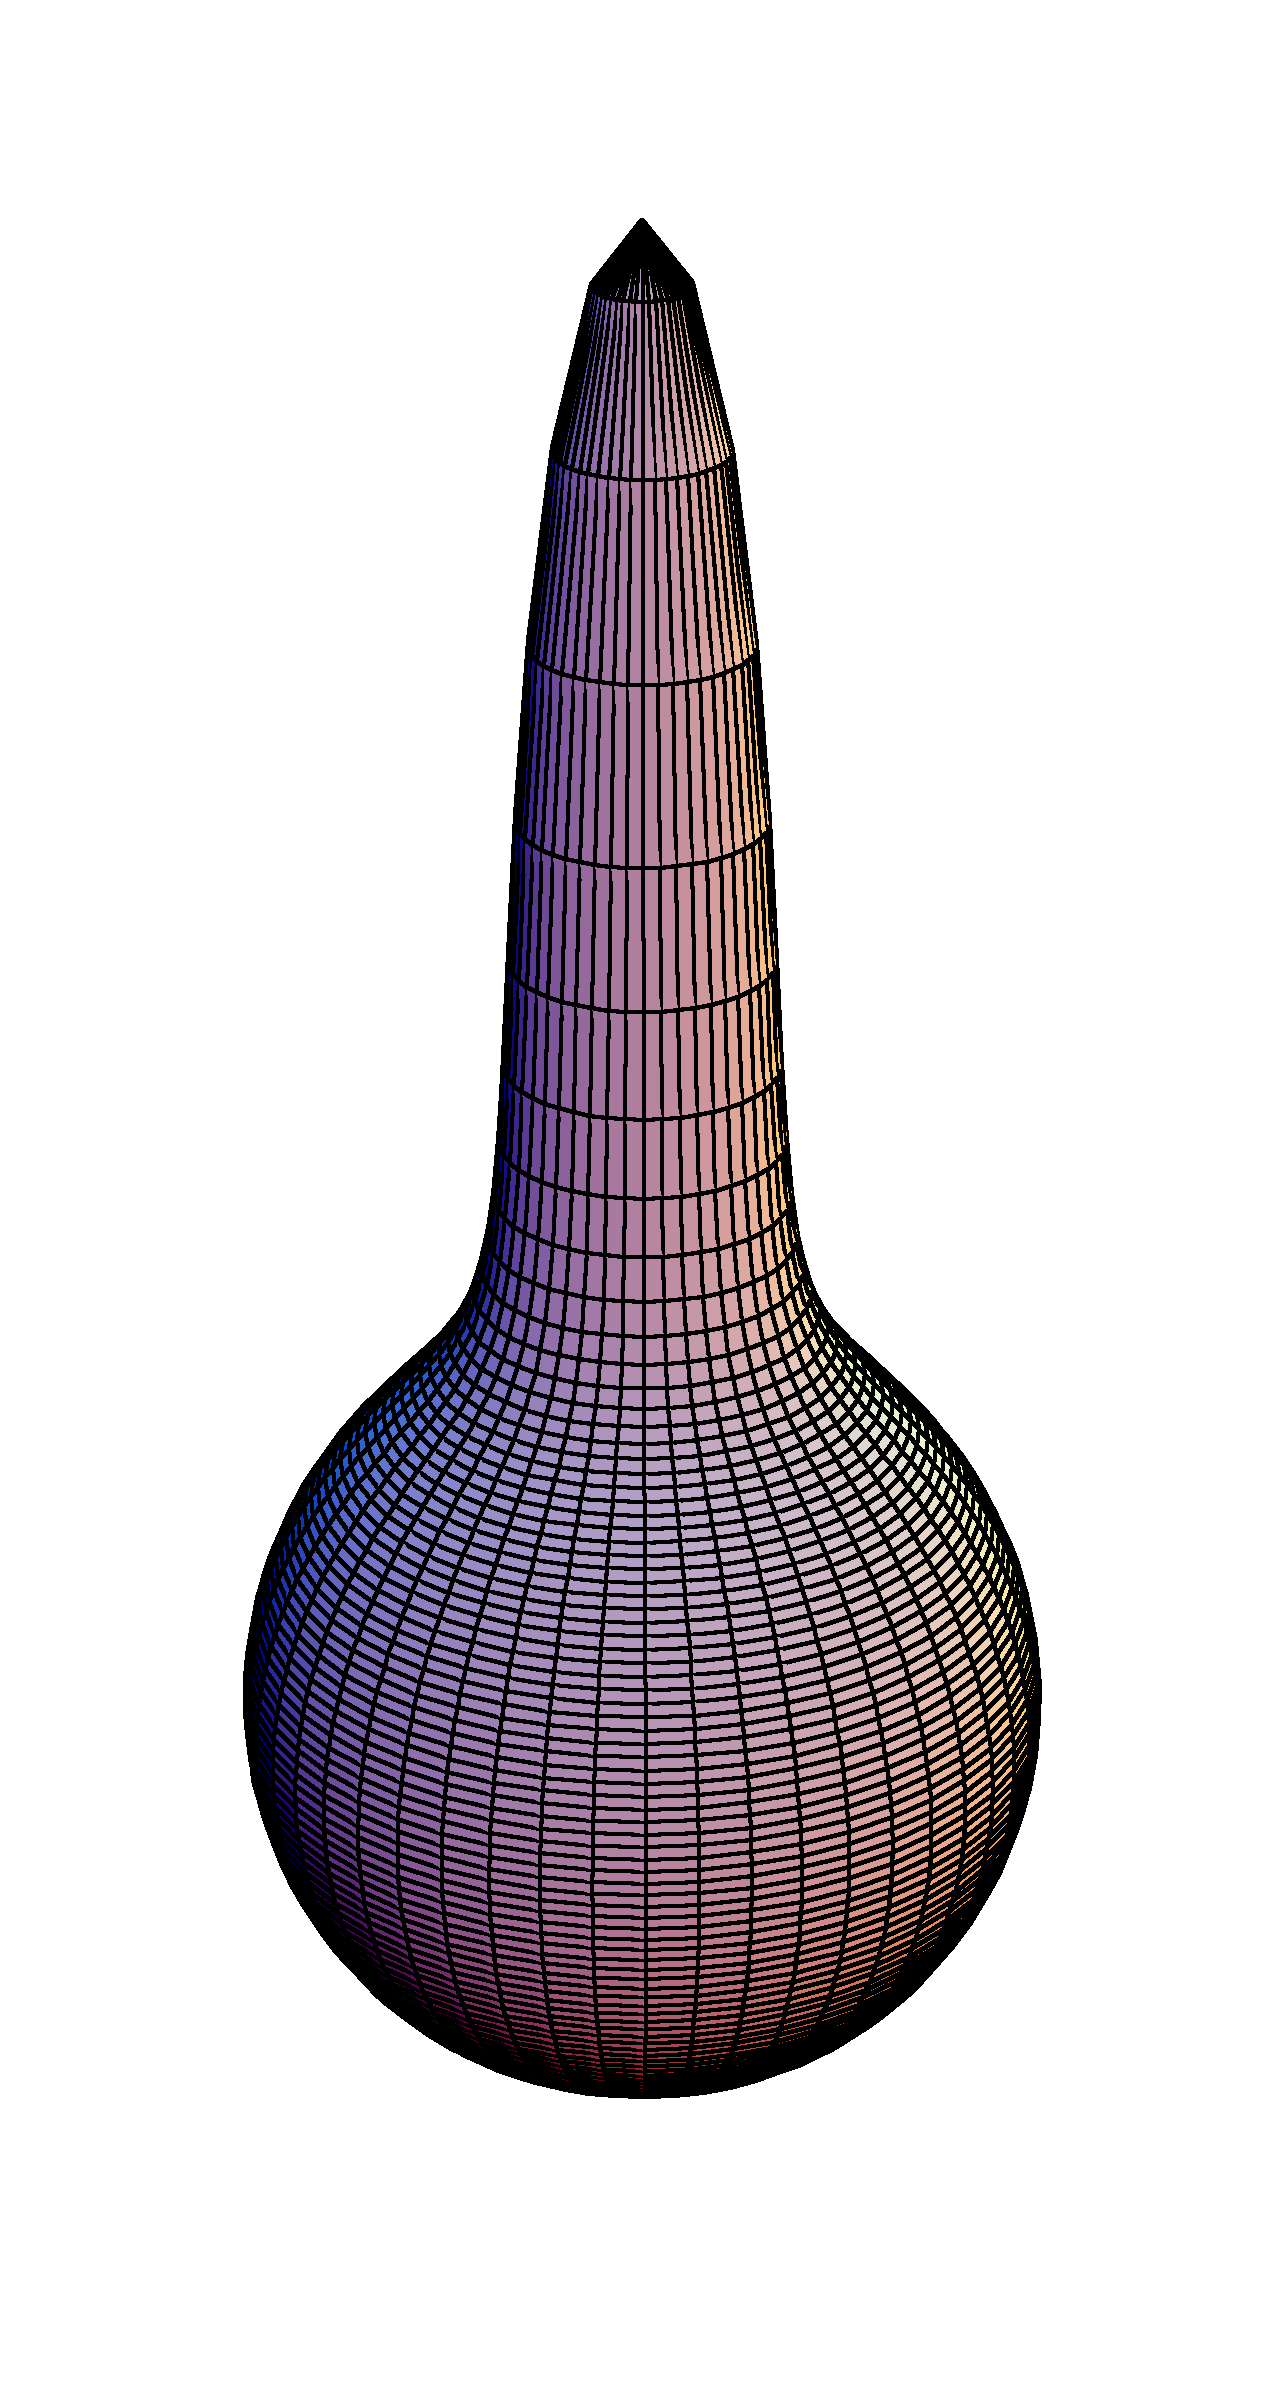
\includegraphics[width=0.5\textwidth]{images/p_085.png}}
%  \caption{The Poisson kernel plotted as a spherical radial basis function on the sphere for different values of $h$.}
%  \label{Basics:Figure:PoissonKernel2}
%\end{figure}

\begin{example}
  We define the \emph{singularity kernel} $S_{h}:\interv{[}{-1}{1}{]} \rightarrow \R$ by
  \[
    \fun{S_{h}}{x} := \frac{1}{2\pi} \frac{1}{\paren{1-2hx+h^2}^{1/2}}  \quad \paren{x \in \interv{[}{-1}{1}{]}}.
  \]
  Using \eqref{Basics:Solution} we obtain
  \[
    \fun{S_{h}}{x} = \sum_{k = 0}^{\infty} \frac{1}{2\pi} h^k \fun{P_k}{x}
  \]
  and therefore
  \[
    \fun{S_{h}^{\wedge}}{k} = \frac{2k+1}{2} h^k.
  \]
  See Figure \ref{Basics:Figure:SingularityKernel} and for more information \cite[pp. 112]{frgesc}.
\end{example}

\begin{figure}[tbp]
  \centering
  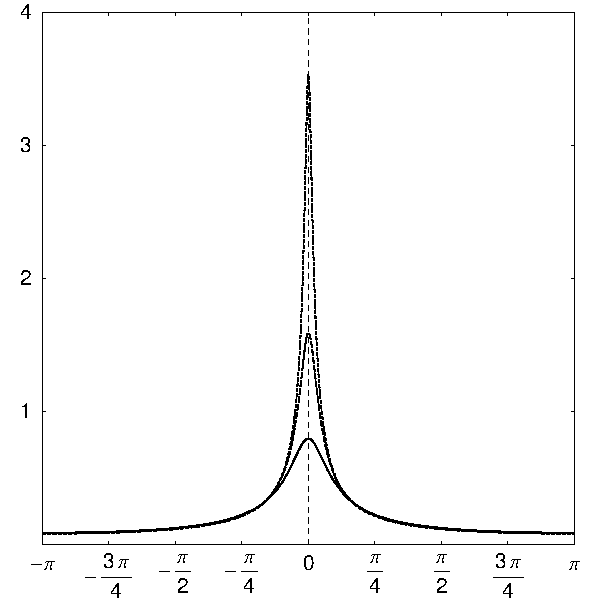
\includegraphics[width=0.7\textwidth]{images/singularity}
  \caption{The singularity kernel $\fun{S_{h}}{\cos\theta}$ for $h = 0.8,0.9,0.95$ and $\theta \in \interv{[}{-\pi}{\pi}{]}$.}
  \label{Basics:Figure:SingularityKernel}
\end{figure}

\begin{example}
  The \emph{Gauss-Weierstra� kernel} $W_{\rho}: \interv{[}{-\pi}{\pi}{]} \rightarrow \R$ is defined by
  \[
    \fun{W_{\rho}}{x} := \sum_{k=0}^{\infty} \e^{-k(k+1)\rho} \frac{2k+1}{4\pi} \fun{P_{k}}{x} \quad \paren{x \in \interv{[}{-1}{1}{]}}.
  \]
  Results due to Bochner (\cite{bochner1950},\cite{bochner1954}) assure $\fun{W_{\rho}}{x} \ge 0$ and we have
  \[
    \int_{\twosphere} \fun{W_{\rho}}{\V{\eta} \cdot \V{\xi}} \dx \V{\xi} = 1.
  \]
  For further properties we refer to \cite{frgesc} again. The kernel function $W_{\rho}$ is illustrated in Figure \ref{Basics:Figure:GaussWeierstrassKernel}.
\end{example}

\begin{figure}[tb]
  \centering
  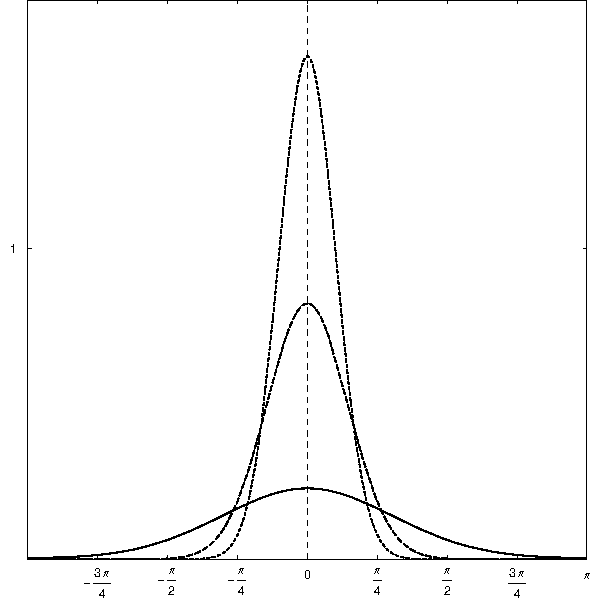
\includegraphics[width=0.7\textwidth]{images/gaussweierstrass}
  \caption{The Gauss-Weierstra� kernel $\fun{W_{\rho}}{\cos\theta}$ for $\rho = 0.4,0.1,0.05$ and $\theta \in \interv{[}{-\pi}{\pi}{]}$.}
  \label{Basics:Figure:GaussWeierstrassKernel}
\end{figure}

\begin{example}
  The locally supported kernel $L_{h,\lambda}: \interv{[}{-1}{1}{]} \rightarrow \R$ mentioned in \cite{frsc} and defined by
  \[
    \fun{L_{h,\lambda}}{x} := 
      \left\{\begin{array}{l@{\quad \text{if} \quad}l} 
                                              0 & -1 \le x \le h, \\
        \frac{\lambda+1}{2\pi(1-h)^{\lambda+1}}\paren{x-h}^{\lambda} &  h   < x \le 1,
      \end{array}\right.
  \]
  has the recursively defined symbol $\fun{L_{h,\lambda}^{\wedge}}{k}$ with
\begin{eqnarray*}
    \fun{L_{h,\lambda}^{\wedge}}{0} & = & 1,\\
    \paren{\lambda+1} \fun{L_{h,\lambda}^{\wedge}}{1} & = & \paren{\lambda + 1 + h},\\
    \paren{k+\lambda+2} \fun{L_{h,\lambda}^{\wedge}}{k+1} & = & \paren{2k+1} h \fun{L_{h,\lambda}^{\wedge}}{k} - \paren{k-\lambda-1} \fun{L_{h,\lambda}^{\wedge}}{k-1} 
    \quad \paren{k = 1,2,\ldots}.
\end{eqnarray*}
  Figure \ref{Basics:Figure:LKernel} shows the function $L_{h,\lambda}$ for different values $h$ and $\lambda$.
\end{example}

\begin{figure}[tb]
  \centering
   \subfigure[$\lambda=1.5$]
     {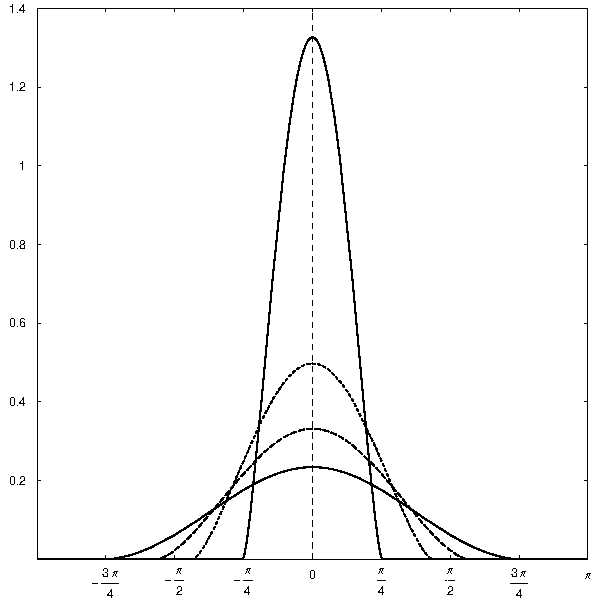
\includegraphics[width=0.33\textwidth]{images/locsup4}}\hfill
   \subfigure[$\lambda=1.0$]
     {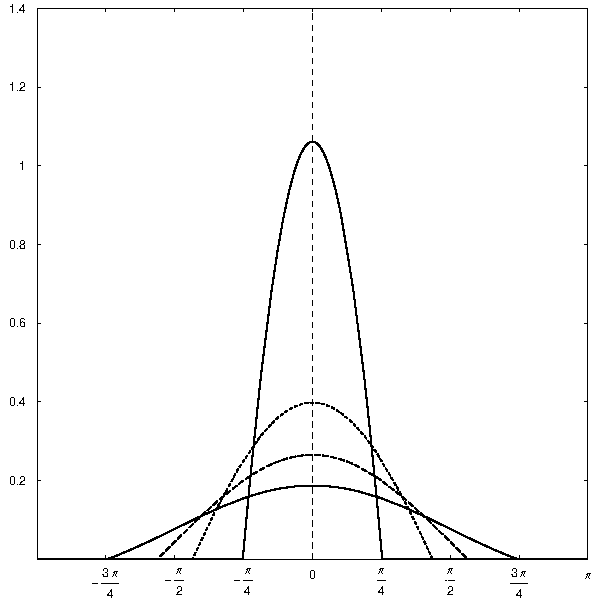
\includegraphics[width=0.33\textwidth]{images/locsup3}}\\
   \subfigure[$\lambda=0.5$]
     {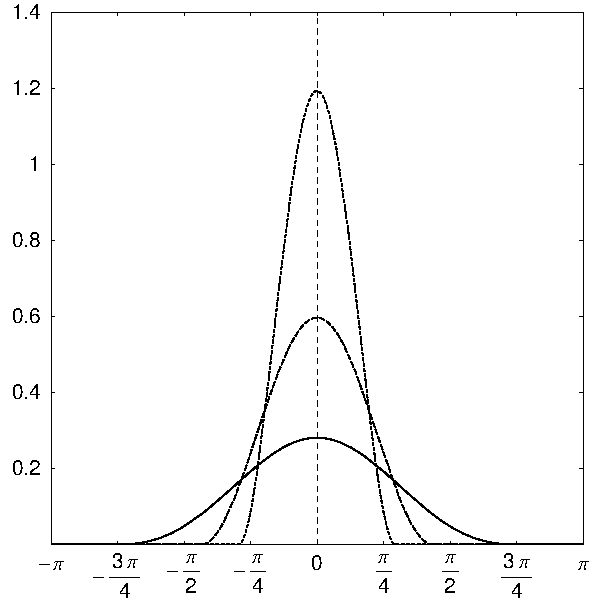
\includegraphics[width=0.33\textwidth]{images/locsup2}}\hfill
   \subfigure[$\lambda=0.2$]
     {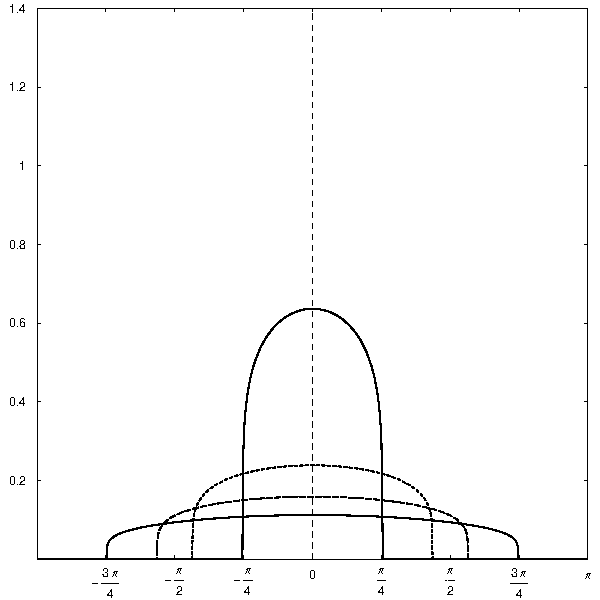
\includegraphics[width=0.33\textwidth]{images/locsup1}}
  \caption{The kernel $L_{h,\lambda}$ for $h = -0.7, -0.2, 0.2, 0.7$ and different values of $\lambda$.}
  \label{Basics:Figure:LKernel}
\end{figure}
\section{Spherical Radial Basis Functions}
\label{Basics:SphericalKernels}

\emph{Spherical radial basis basis functions} are the spherical counterpart of radial basis functions in Euclidean spaces. 
Generally, one starts with a function $K$ from $\Ln{2}{\interv{[}{-1}{1}{]}}$
%$: \interv{[}{-1}{1}{]} \rightarrow \C$ 
and defines for fixed $\V{\eta} \in \twosphere$ the $\V{\eta}$-zonal function 
\[
  \fun{K}{\V{\eta} \: \cdot}: \twosphere \rightarrow \C,\ \V{\xi} \mapsto \fun{K}{\V{\eta} \cdot \V{\xi}} \quad \paren{\V{\xi} \in \twosphere}.\] 
%by \[ \fun{K_{\V{\eta}}}{\V{\xi}} := \fun{G}{\V{\eta} \cdot \V{\xi}}.\]
By means of the \emph{Funk-Hecke formula} (see \cite[pp. 60]{frgesc}) we obtain for fixed $k \in \NZ$
\[
  \scalarproduct{\fun{K}{\V{\eta} \: \cdot}}{Y_{k}^n} = \int_{\twosphere} \fun{K}{\V{\eta} \cdot \V{\xi}} \overline{\fun{Y_{k}^n}{\V{\xi}}} \: \dx \V{\xi} = \fun{K^{\wedge}}{k} \overline{\fun{Y_{k}^n}{\V{\eta}}} \quad \paren{n=-k,\ldots,k},
\]
where the \emph{Legendre transform}, i.e. the \emph{symbol} of $K$, is given by
\[
  \fun{K^{\wedge}}{k} := 2 \pi \int_{-1}^{1} \fun{K}{x} \fun{P_{k}}{x} \dx x \quad \paren{k \in \NZ}.
\]
%We refer the interested reader to \cite{} and \cite{} for more details.
%The function $G$ can be developed into a series of Legendre polynomials
%\[ \fun{G}{x} = \sum_{k = 0}^{\infty} a_k \fun{P_k}{x}.\]
%where the coefficients $a_k$ are the scalar products
%\[ a_k = \scalarproduct{G}{P_{k}}_{\interv{[}{-1}{1}{]}} = \int_{-1}^{1} \fun{G}{x} \fun{P_k}{x} \dx x.\]
We have therefore 
\begin{equation}
  \label{Basics:Kernel}
  \fun{K}{\V{\eta} \cdot \V{\xi}} = \sum_{k = 0}^{\infty} \sum_{n=-k}^k \fun{K^{\wedge}}{k} \overline{\fun{Y_{k}^n}{\V{\eta}}} \fun{Y_{k}^n}{\V{\xi}} 
\end{equation}
and applying the Addition Theorem from Proposition \ref{Basics:AdditionTheorem}, we obtain for $K$ the orthogonal expansion
\begin{equation}
\label{Basics:OrthogonalKernelExpansion}
  \fun{K}{x} = \sum_{k = 0}^{\infty} \frac{2k+1}{4\pi} \fun{K^{\wedge}}{k} \fun{P_k}{x} \quad \paren{x \in \interv{[}{-1}{1}{]}}.
\end{equation}
%One is often interested in evaluating such an expansion on the sphere in a fast way when dealing with 
%spherical convolution. As an application of the algorithms developed in this text, one can derive 
%an algorithm based on the discrete spherical Fourier transform, as shown in Chapter \ref{}.

\begin{example}
We consider the generating series
\begin{equation}
  \label{Basics:GeneratingFunction}
  \fun{\phi}{h} := \sum_{k = 0}^{\infty} h^k \fun{P_k}{x} \quad \paren{x \in \interv{[}{-1}{1}{]}}
\end{equation}
which is absolutely and uniformly convergent for $h \in
\interv{(}{-1}{1}{)}$ with
\begin{equation}
  \label{Basics:Solution}
  \sum_{k = 0}^{\infty} h^k \fun{P_k}{x} = \frac{1}{\sqrt{1-2hx+h^2}}.
\end{equation}
This follows from the ordinary differential equation
\begin{equation}
\label{Basics:DifferentialEquation}
  \paren{1+h^2-2hx}\fun{\phi'}{h} = \paren{x-h}\fun{\phi}{h}
\end{equation}
obtained by differentiation with respect to $h$ and comparing coefficients in line with \eqref{Basics:GeneratingFunction}. Using the initial 
condition $\fun{\phi}{0}=1$ this yields the unique solution \eqref{Basics:Solution} of \eqref{Basics:DifferentialEquation}.
From this result, the identity
\begin{equation}
  \nonumber
  \sum_{k=0}^{\infty} \paren{2k+1} h^k \fun{P_k}{x} =
  \frac{1-h^2}{\paren{1-2hx+h^2}^{3/2}}
\end{equation}
 follows easily. When $h$ is restricted to $\interv{(}{0}{1}{)}$ the function
$Q_{h}:\interv{[}{-1}{1}{]} \rightarrow \R$, with
\begin{equation}
  \label{PoissonKernel}
  \nonumber
  \fun{Q_{h}}{x} := \frac{1}{4\pi} \frac{1-h^2}{\paren{1-2hx+h^2}^{3/2}} \quad \paren{x \in \interv{[}{-1}{1}{]}},
\end{equation}
is called \emph{Poisson kernel}. The symbol $\fun{Q_{h}^{\wedge}}{k}$ is given by 
\[
  \fun{Q_{h}^{\wedge}}{k} = h^k.
\]
We refer to Figure \ref{Basics:Figure:PoissonKernel} 
%and \ref{Basics:Figure:PoissonKernel2}
for a visual impression and mention that the parameter $h$
allows for controlling the concentration of the function's energy around
$x = 1$. The Poisson kernel is a positive function and normalized with
\[
  \int_{\twosphere} \fun{Q_{h}}{\V{\eta} \cdot \V{\xi}} \dx \V{\xi} = 1 \quad \paren{\V{\eta} \in \twosphere}.
\]
Further properties with respect to localization and smoothness are derived in \cite[pp. 112]{frgesc}.
\end{example}

\begin{figure}[tbp]
  \centering
  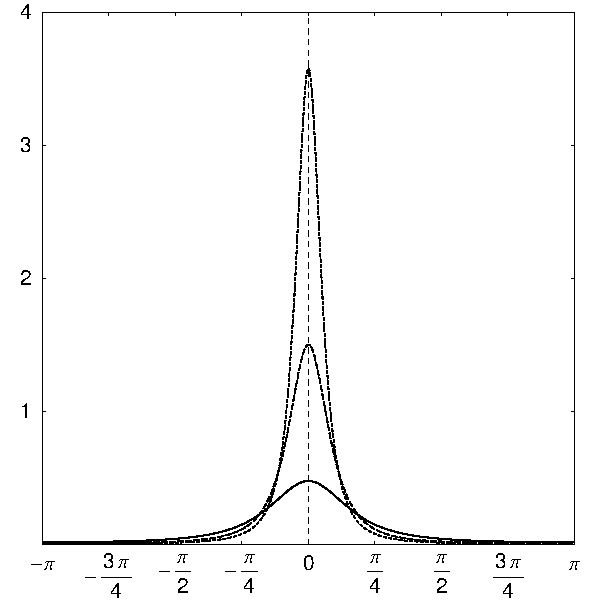
\includegraphics[width=0.7\textwidth]{images/poisson}
  \caption{The Poisson kernel $\fun{Q_{h}}{\cos\theta}$ for $h = 0.5,0.7,0.8$ and $\theta \in \interv{[}{-\pi}{\pi}{]}$.}
  \label{Basics:Figure:PoissonKernel}
\end{figure}

%\begin{figure}[htb]
%  \centering
%   \subfigure[$h=0.70$]
%     {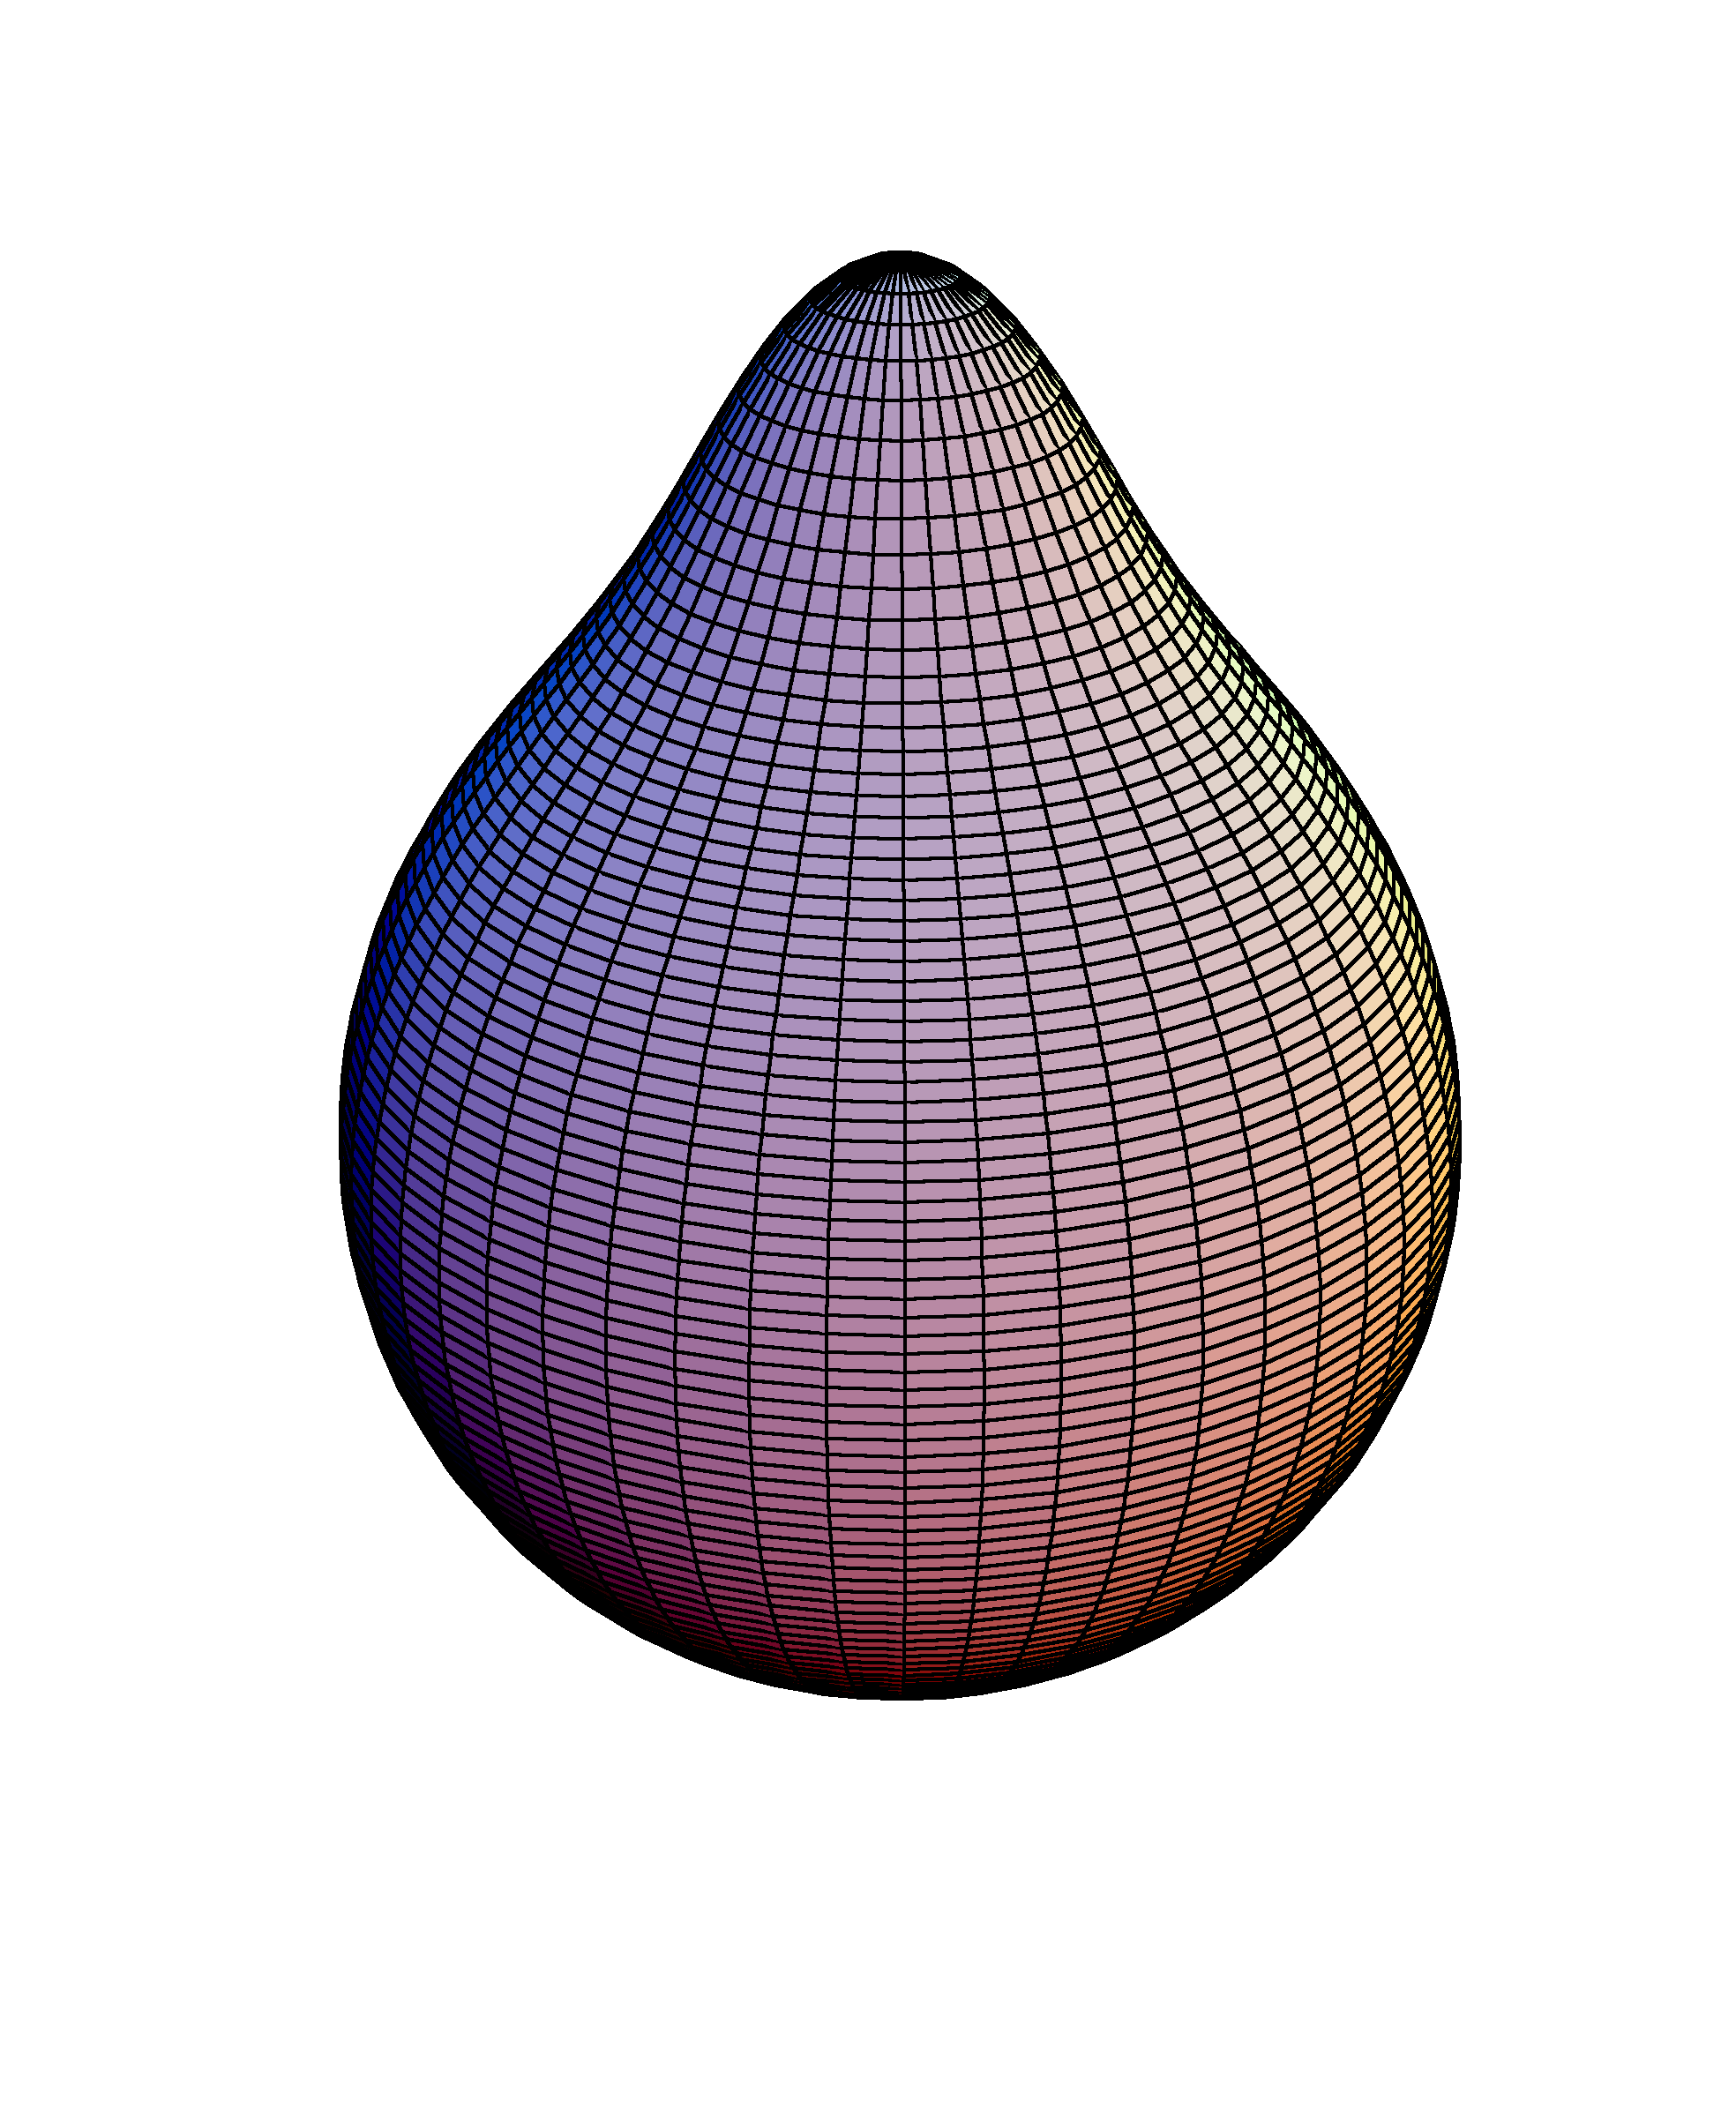
\includegraphics[width=0.5\textwidth]{images/p_070.png}}\hfill
%   \subfigure[$h=0.75$]
%     {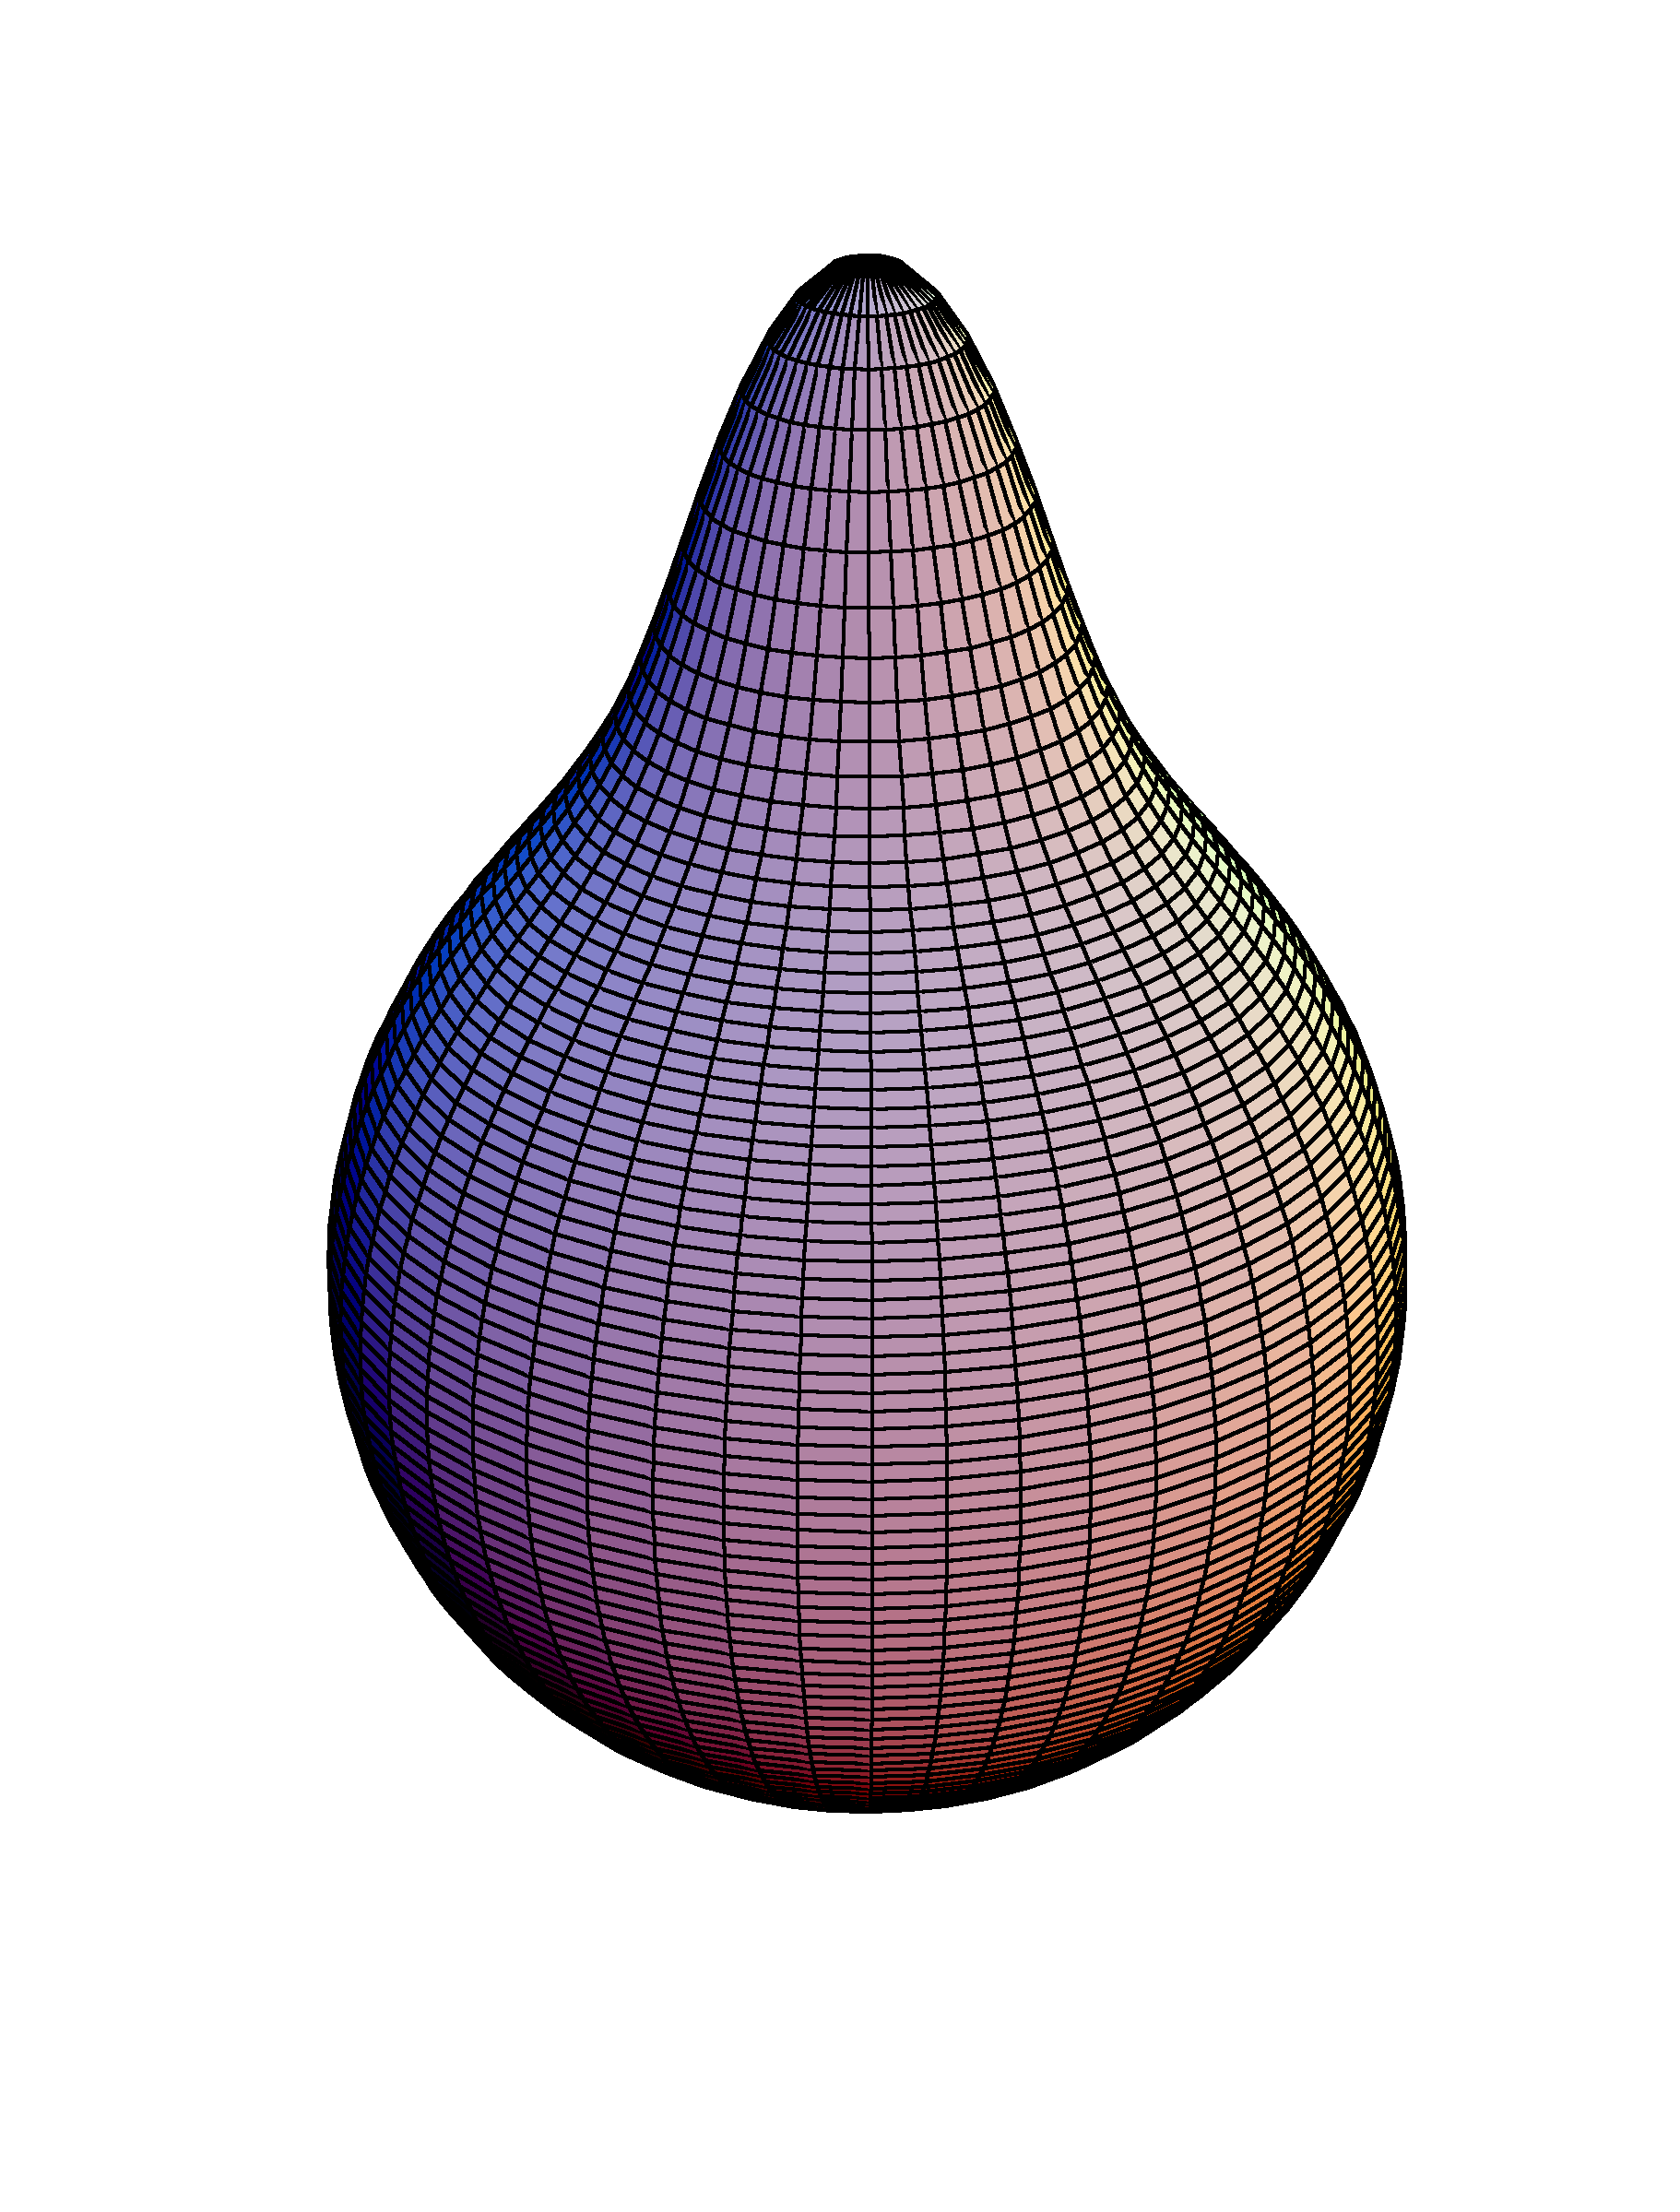
\includegraphics[width=0.5\textwidth]{images/p_075.png}}\\
%   \subfigure[$h=0.80$]
%     {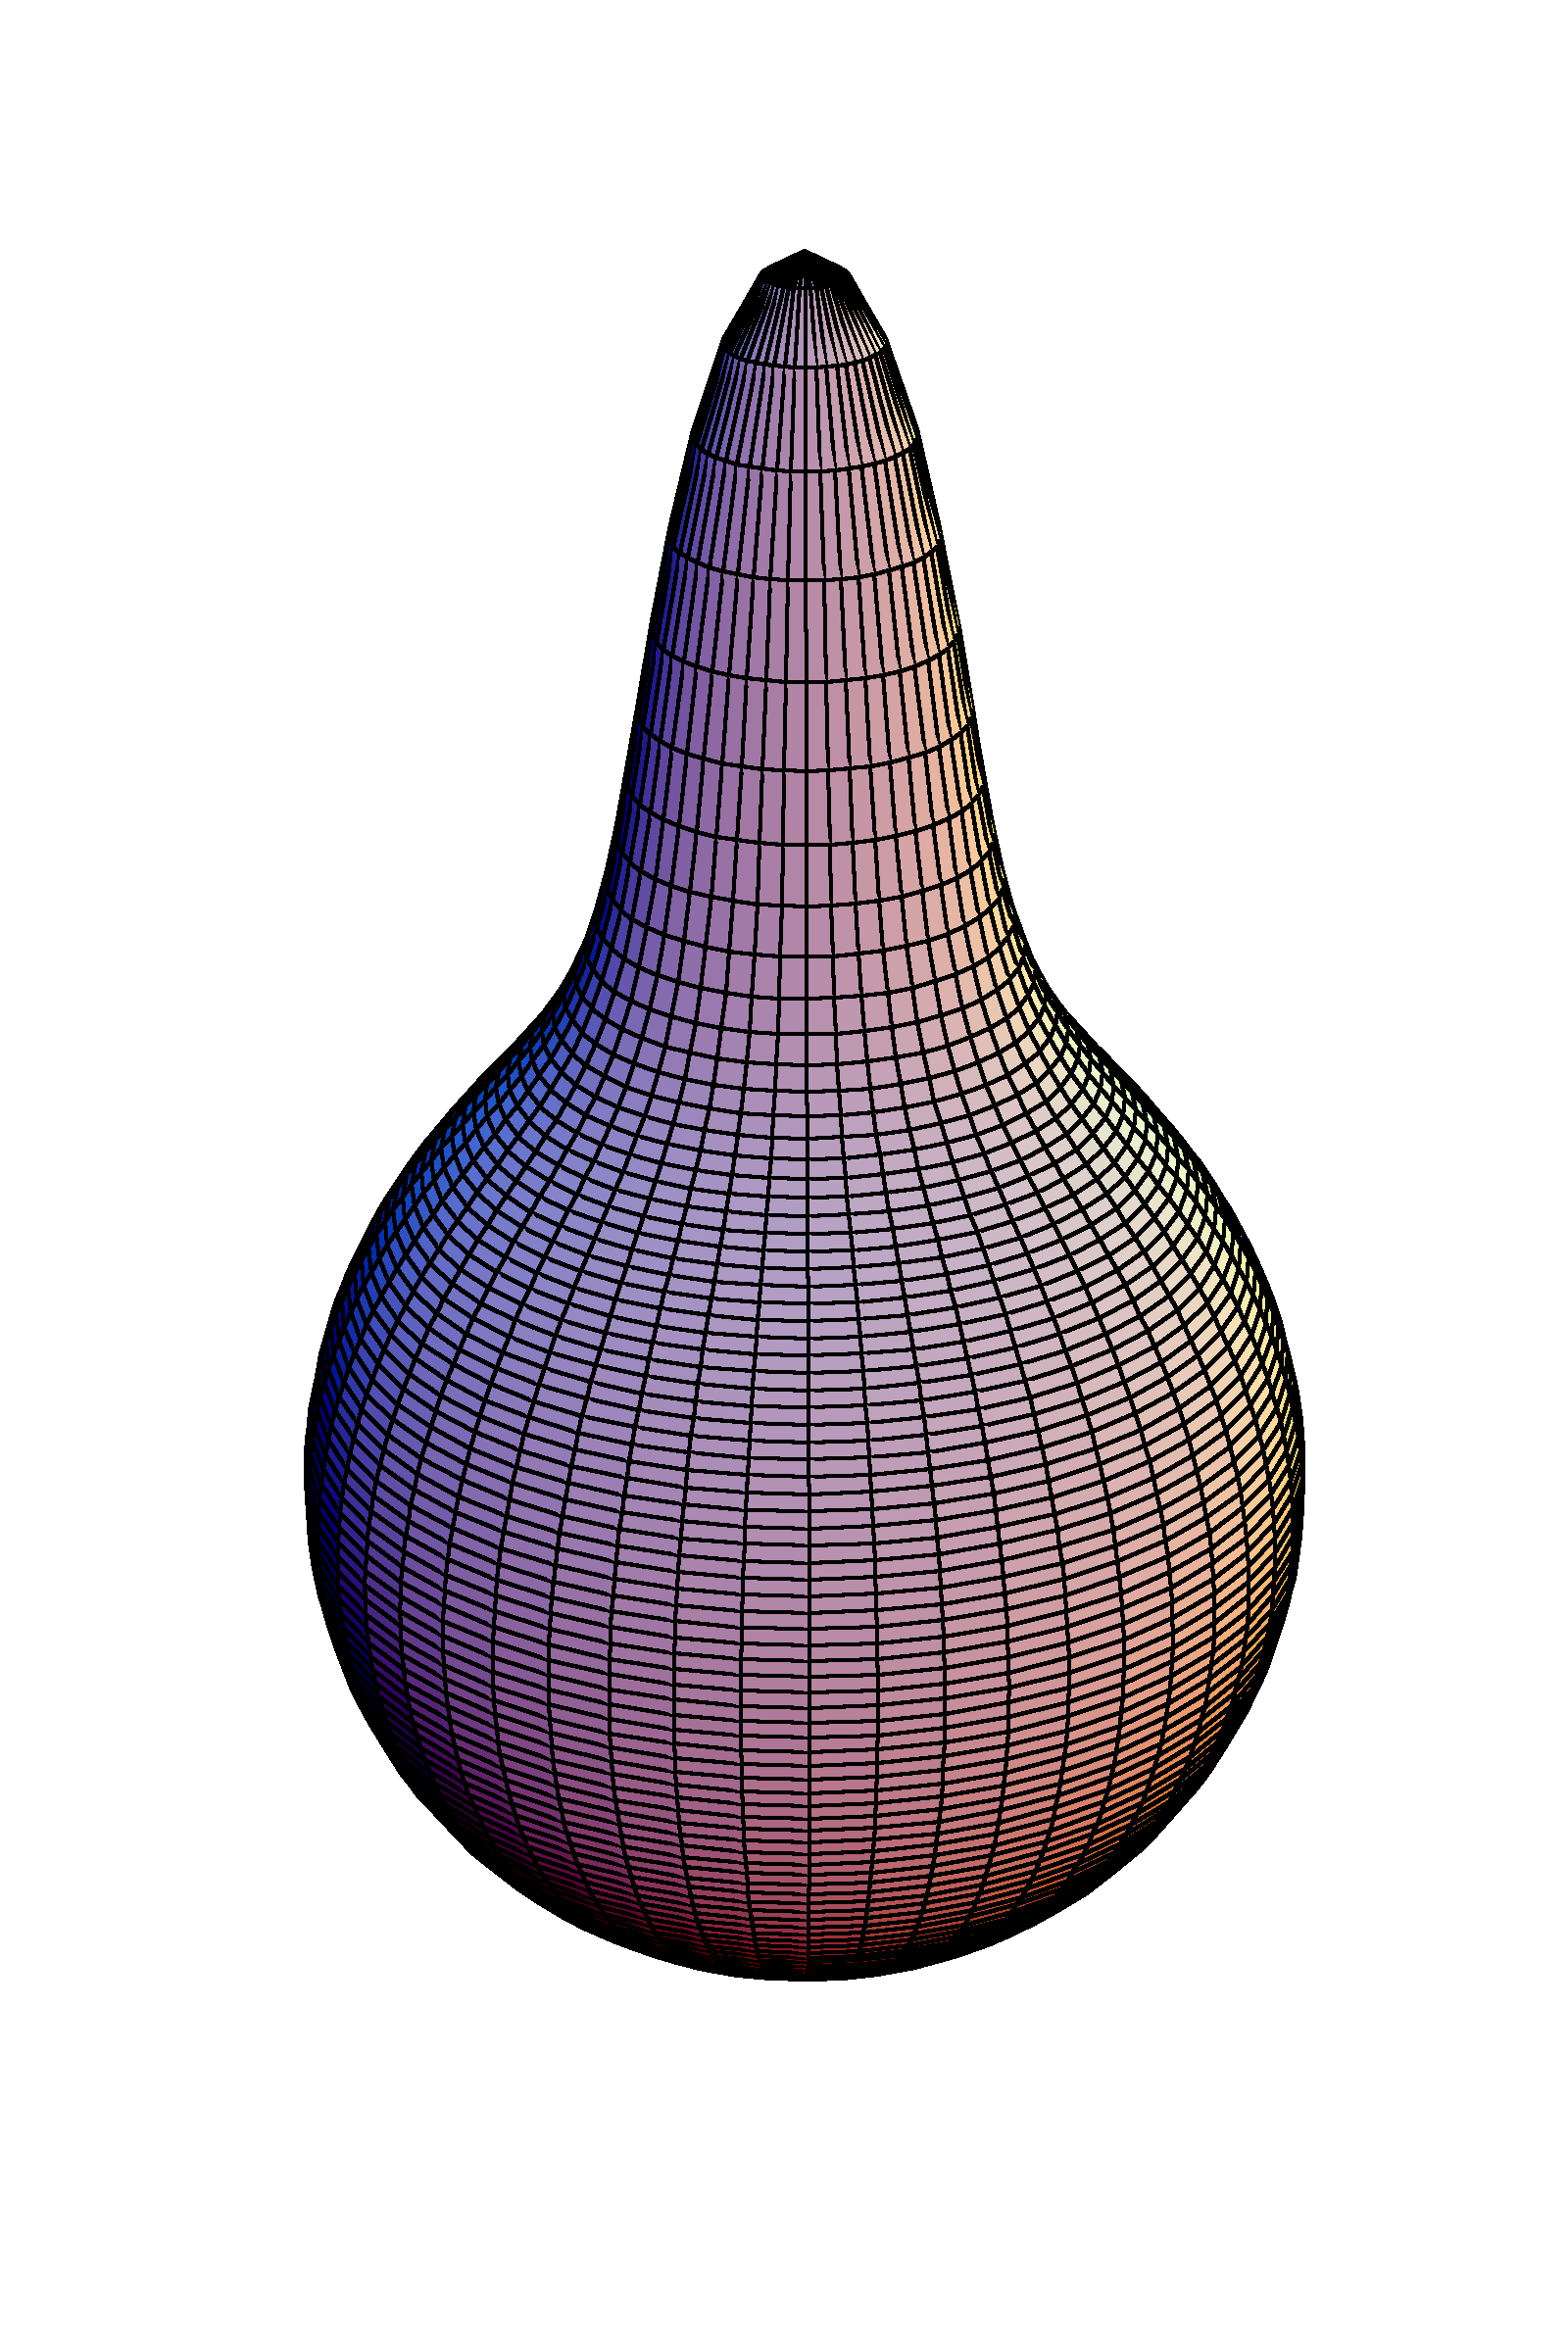
\includegraphics[width=0.5\textwidth]{images/p_080.png}}\hfill
%   \subfigure[$h=0.85$]
%     {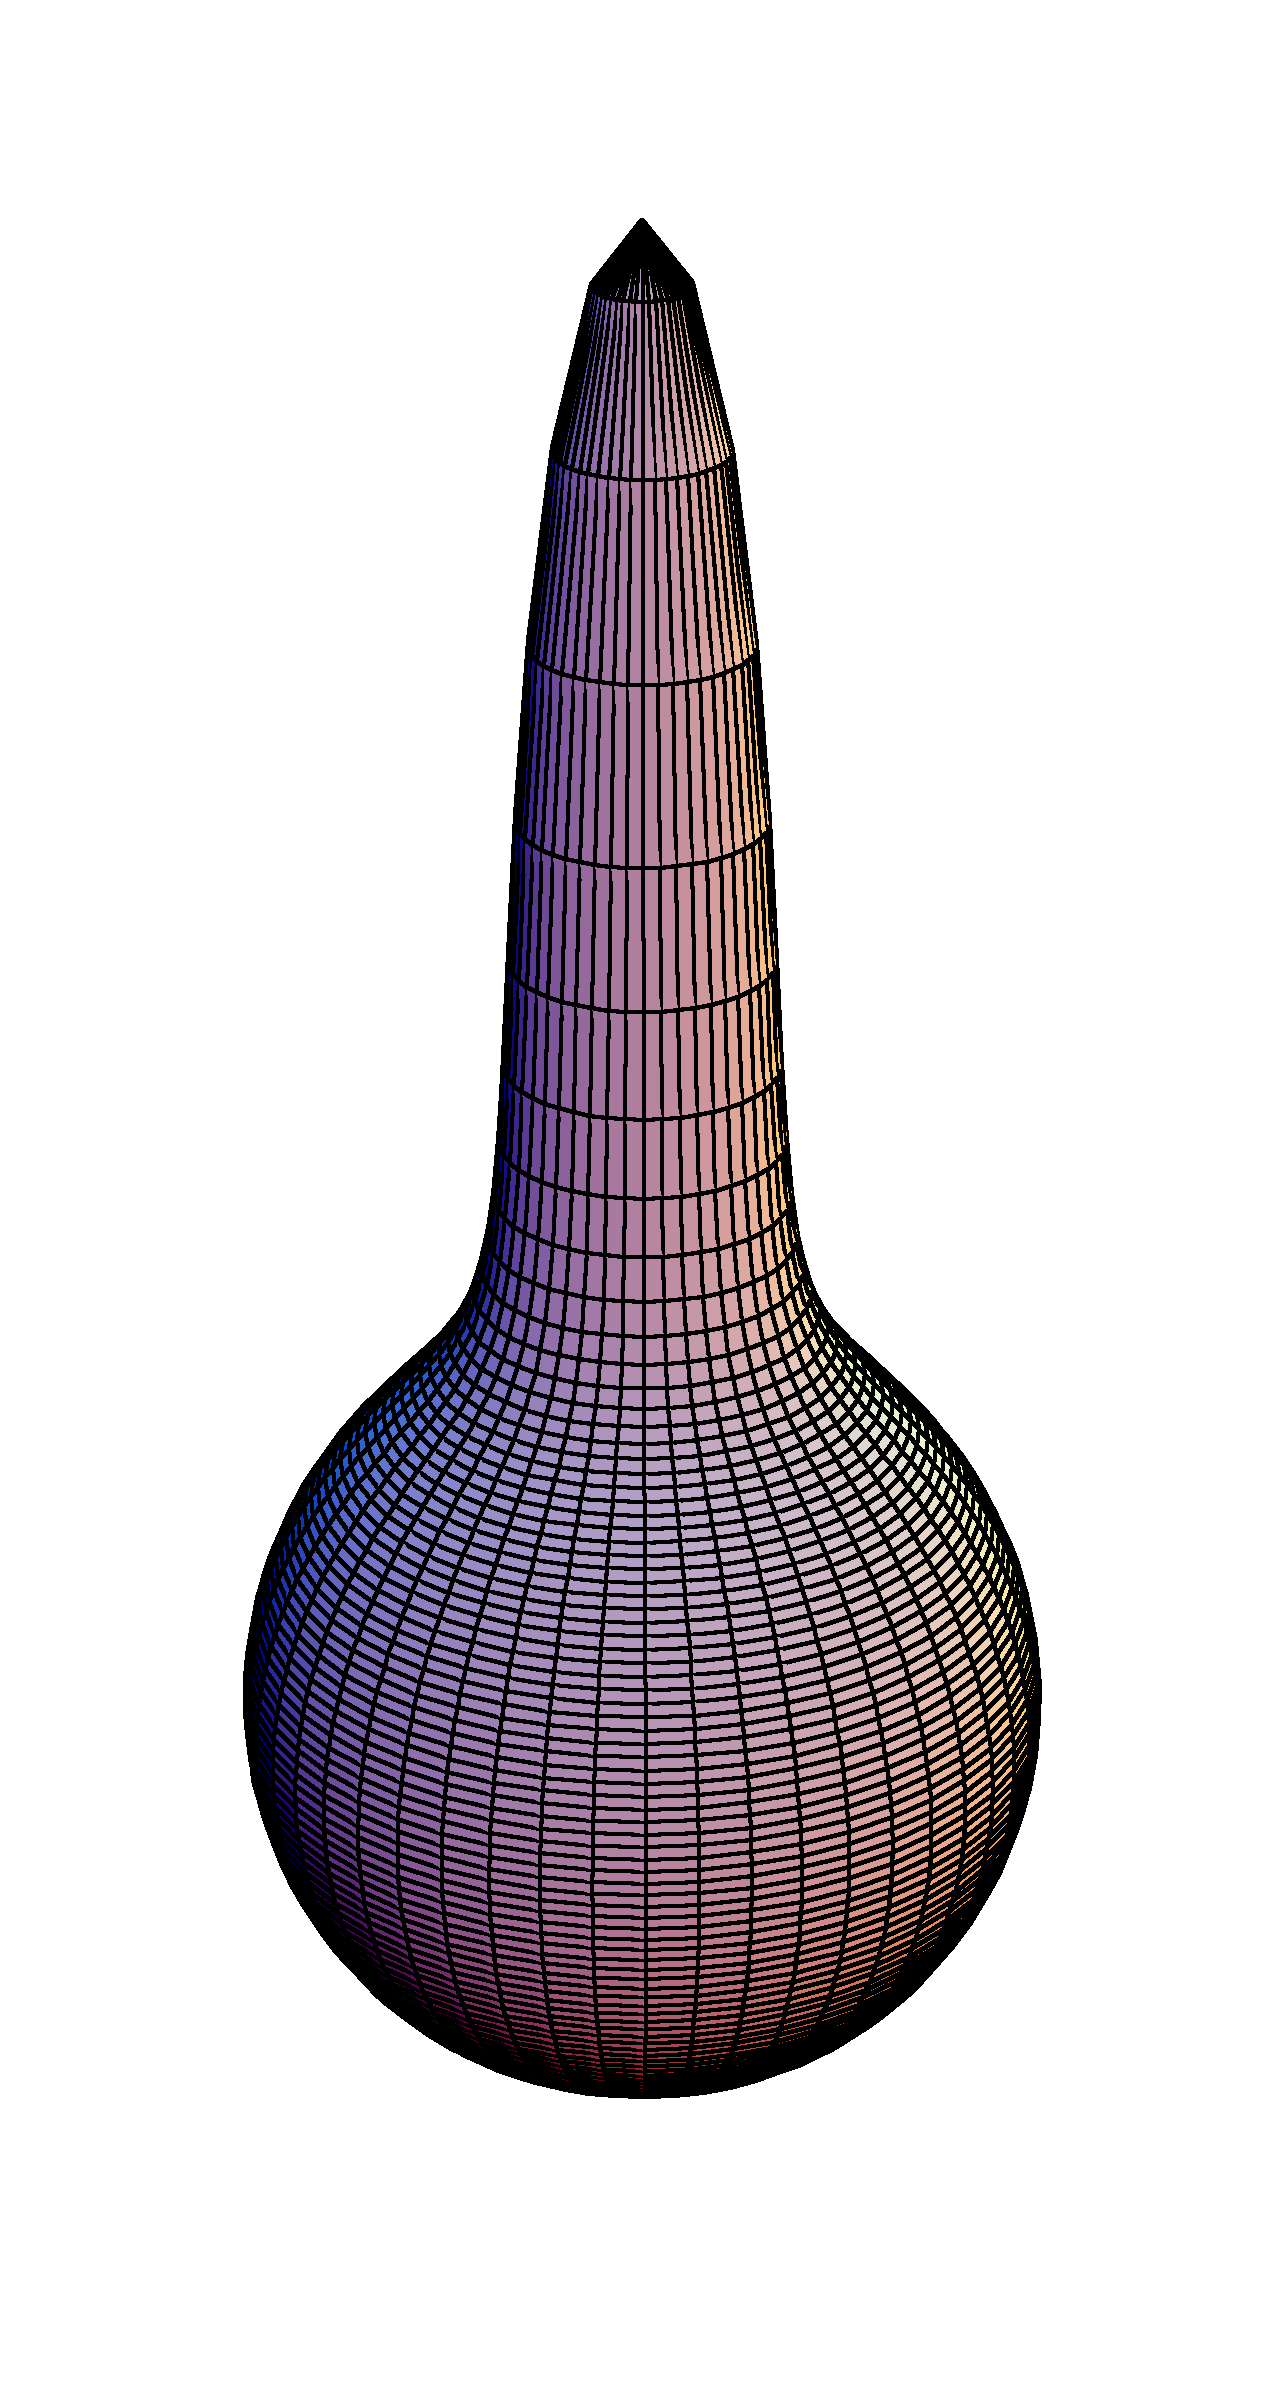
\includegraphics[width=0.5\textwidth]{images/p_085.png}}
%  \caption{The Poisson kernel plotted as a spherical radial basis function on the sphere for different values of $h$.}
%  \label{Basics:Figure:PoissonKernel2}
%\end{figure}

\begin{example}
  We define the \emph{singularity kernel} $S_{h}:\interv{[}{-1}{1}{]} \rightarrow \R$ by
  \[
    \fun{S_{h}}{x} := \frac{1}{2\pi} \frac{1}{\paren{1-2hx+h^2}^{1/2}}  \quad \paren{x \in \interv{[}{-1}{1}{]}}.
  \]
  Using \eqref{Basics:Solution} we obtain
  \[
    \fun{S_{h}}{x} = \sum_{k = 0}^{\infty} \frac{1}{2\pi} h^k \fun{P_k}{x}
  \]
  and therefore
  \[
    \fun{S_{h}^{\wedge}}{k} = \frac{2k+1}{2} h^k.
  \]
  See Figure \ref{Basics:Figure:SingularityKernel} and for more information \cite[pp. 112]{frgesc}.
\end{example}

\begin{figure}[tbp]
  \centering
  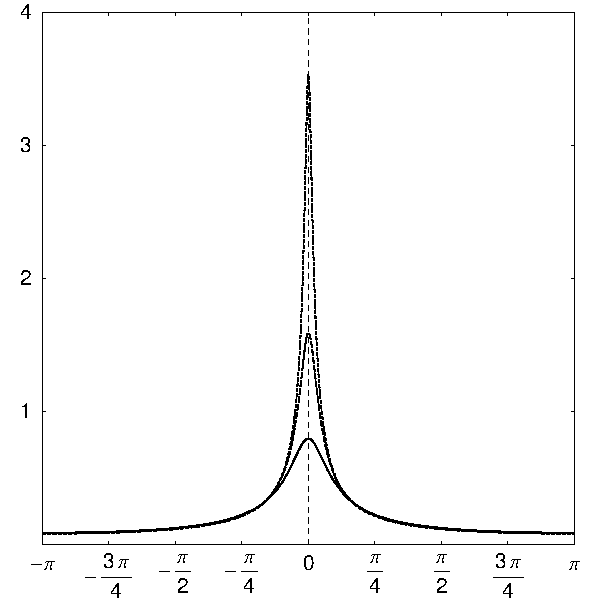
\includegraphics[width=0.7\textwidth]{images/singularity}
  \caption{The singularity kernel $\fun{S_{h}}{\cos\theta}$ for $h = 0.8,0.9,0.95$ and $\theta \in \interv{[}{-\pi}{\pi}{]}$.}
  \label{Basics:Figure:SingularityKernel}
\end{figure}

\begin{example}
  The \emph{Gauss-Weierstra� kernel} $W_{\rho}: \interv{[}{-\pi}{\pi}{]} \rightarrow \R$ is defined by
  \[
    \fun{W_{\rho}}{x} := \sum_{k=0}^{\infty} \e^{-k(k+1)\rho} \frac{2k+1}{4\pi} \fun{P_{k}}{x} \quad \paren{x \in \interv{[}{-1}{1}{]}}.
  \]
  Results due to Bochner (\cite{bochner1950},\cite{bochner1954}) assure $\fun{W_{\rho}}{x} \ge 0$ and we have
  \[
    \int_{\twosphere} \fun{W_{\rho}}{\V{\eta} \cdot \V{\xi}} \dx \V{\xi} = 1.
  \]
  For further properties we refer to \cite{frgesc} again. The kernel function $W_{\rho}$ is illustrated in Figure \ref{Basics:Figure:GaussWeierstrassKernel}.
\end{example}

\begin{figure}[tb]
  \centering
  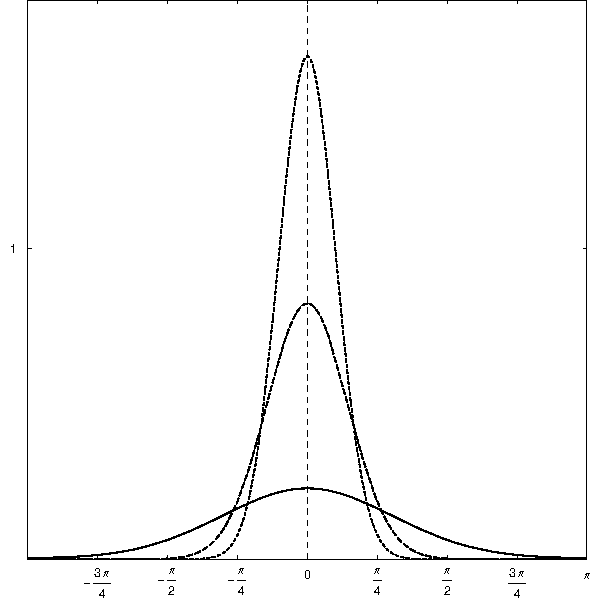
\includegraphics[width=0.7\textwidth]{images/gaussweierstrass}
  \caption{The Gauss-Weierstra� kernel $\fun{W_{\rho}}{\cos\theta}$ for $\rho = 0.4,0.1,0.05$ and $\theta \in \interv{[}{-\pi}{\pi}{]}$.}
  \label{Basics:Figure:GaussWeierstrassKernel}
\end{figure}

\begin{example}
  The locally supported kernel $L_{h,\lambda}: \interv{[}{-1}{1}{]} \rightarrow \R$ mentioned in \cite{frsc} and defined by
  \[
    \fun{L_{h,\lambda}}{x} := 
      \left\{\begin{array}{l@{\quad \text{if} \quad}l} 
                                              0 & -1 \le x \le h, \\
        \frac{\lambda+1}{2\pi(1-h)^{\lambda+1}}\paren{x-h}^{\lambda} &  h   < x \le 1,
      \end{array}\right.
  \]
  has the recursively defined symbol $\fun{L_{h,\lambda}^{\wedge}}{k}$ with
\begin{eqnarray*}
    \fun{L_{h,\lambda}^{\wedge}}{0} & = & 1,\\
    \paren{\lambda+1} \fun{L_{h,\lambda}^{\wedge}}{1} & = & \paren{\lambda + 1 + h},\\
    \paren{k+\lambda+2} \fun{L_{h,\lambda}^{\wedge}}{k+1} & = & \paren{2k+1} h \fun{L_{h,\lambda}^{\wedge}}{k} - \paren{k-\lambda-1} \fun{L_{h,\lambda}^{\wedge}}{k-1} 
    \quad \paren{k = 1,2,\ldots}.
\end{eqnarray*}
  Figure \ref{Basics:Figure:LKernel} shows the function $L_{h,\lambda}$ for different values $h$ and $\lambda$.
\end{example}

\begin{figure}[tb]
  \centering
   \subfigure[$\lambda=1.5$]
     {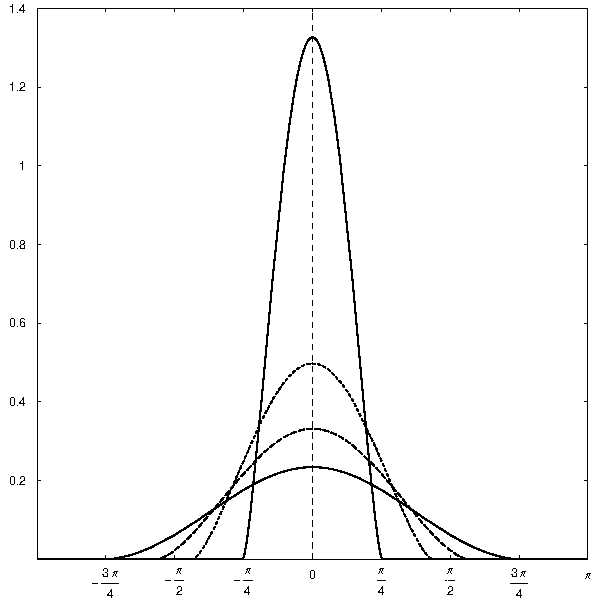
\includegraphics[width=0.33\textwidth]{images/locsup4}}\hfill
   \subfigure[$\lambda=1.0$]
     {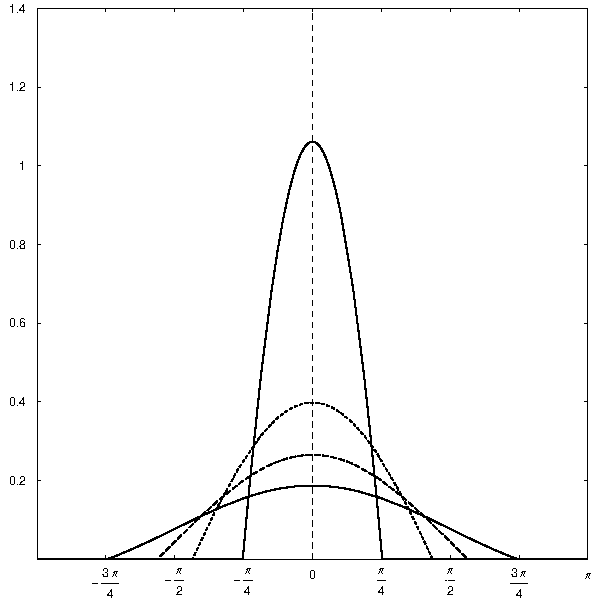
\includegraphics[width=0.33\textwidth]{images/locsup3}}\\
   \subfigure[$\lambda=0.5$]
     {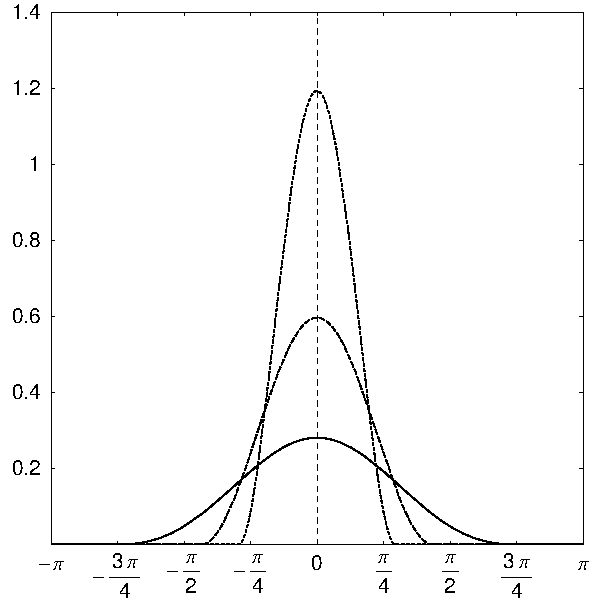
\includegraphics[width=0.33\textwidth]{images/locsup2}}\hfill
   \subfigure[$\lambda=0.2$]
     {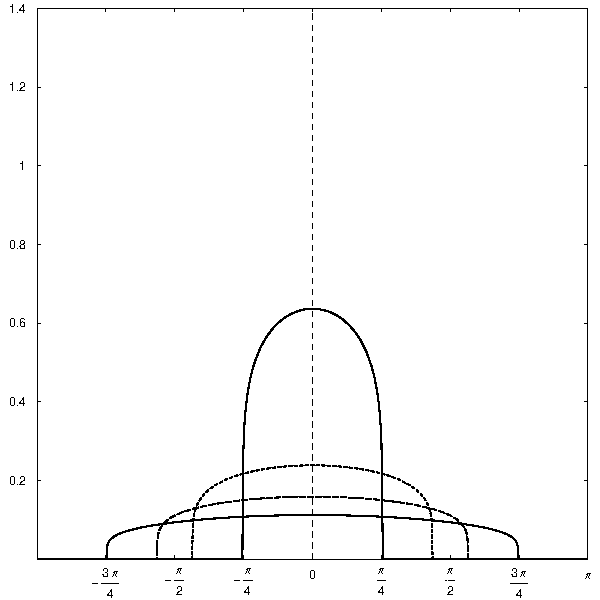
\includegraphics[width=0.33\textwidth]{images/locsup1}}
  \caption{The kernel $L_{h,\lambda}$ for $h = -0.7, -0.2, 0.2, 0.7$ and different values of $\lambda$.}
  \label{Basics:Figure:LKernel}
\end{figure}
\section{Spherical Radial Basis Functions}
\label{Basics:SphericalKernels}

\emph{Spherical radial basis basis functions} are the spherical counterpart of radial basis functions in Euclidean spaces. 
Generally, one starts with a function $K$ from $\Ln{2}{\interv{[}{-1}{1}{]}}$
%$: \interv{[}{-1}{1}{]} \rightarrow \C$ 
and defines for fixed $\V{\eta} \in \twosphere$ the $\V{\eta}$-zonal function 
\[
  \fun{K}{\V{\eta} \: \cdot}: \twosphere \rightarrow \C,\ \V{\xi} \mapsto \fun{K}{\V{\eta} \cdot \V{\xi}} \quad \paren{\V{\xi} \in \twosphere}.\] 
%by \[ \fun{K_{\V{\eta}}}{\V{\xi}} := \fun{G}{\V{\eta} \cdot \V{\xi}}.\]
By means of the \emph{Funk-Hecke formula} (see \cite[pp. 60]{frgesc}) we obtain for fixed $k \in \NZ$
\[
  \scalarproduct{\fun{K}{\V{\eta} \: \cdot}}{Y_{k}^n} = \int_{\twosphere} \fun{K}{\V{\eta} \cdot \V{\xi}} \overline{\fun{Y_{k}^n}{\V{\xi}}} \: \dx \V{\xi} = \fun{K^{\wedge}}{k} \overline{\fun{Y_{k}^n}{\V{\eta}}} \quad \paren{n=-k,\ldots,k},
\]
where the \emph{Legendre transform}, i.e. the \emph{symbol} of $K$, is given by
\[
  \fun{K^{\wedge}}{k} := 2 \pi \int_{-1}^{1} \fun{K}{x} \fun{P_{k}}{x} \dx x \quad \paren{k \in \NZ}.
\]
%We refer the interested reader to \cite{} and \cite{} for more details.
%The function $G$ can be developed into a series of Legendre polynomials
%\[ \fun{G}{x} = \sum_{k = 0}^{\infty} a_k \fun{P_k}{x}.\]
%where the coefficients $a_k$ are the scalar products
%\[ a_k = \scalarproduct{G}{P_{k}}_{\interv{[}{-1}{1}{]}} = \int_{-1}^{1} \fun{G}{x} \fun{P_k}{x} \dx x.\]
We have therefore 
\begin{equation}
  \label{Basics:Kernel}
  \fun{K}{\V{\eta} \cdot \V{\xi}} = \sum_{k = 0}^{\infty} \sum_{n=-k}^k \fun{K^{\wedge}}{k} \overline{\fun{Y_{k}^n}{\V{\eta}}} \fun{Y_{k}^n}{\V{\xi}} 
\end{equation}
and applying the Addition Theorem from Proposition \ref{Basics:AdditionTheorem}, we obtain for $K$ the orthogonal expansion
\begin{equation}
\label{Basics:OrthogonalKernelExpansion}
  \fun{K}{x} = \sum_{k = 0}^{\infty} \frac{2k+1}{4\pi} \fun{K^{\wedge}}{k} \fun{P_k}{x} \quad \paren{x \in \interv{[}{-1}{1}{]}}.
\end{equation}
%One is often interested in evaluating such an expansion on the sphere in a fast way when dealing with 
%spherical convolution. As an application of the algorithms developed in this text, one can derive 
%an algorithm based on the discrete spherical Fourier transform, as shown in Chapter \ref{}.

\begin{example}
We consider the generating series
\begin{equation}
  \label{Basics:GeneratingFunction}
  \fun{\phi}{h} := \sum_{k = 0}^{\infty} h^k \fun{P_k}{x} \quad \paren{x \in \interv{[}{-1}{1}{]}}
\end{equation}
which is absolutely and uniformly convergent for $h \in
\interv{(}{-1}{1}{)}$ with
\begin{equation}
  \label{Basics:Solution}
  \sum_{k = 0}^{\infty} h^k \fun{P_k}{x} = \frac{1}{\sqrt{1-2hx+h^2}}.
\end{equation}
This follows from the ordinary differential equation
\begin{equation}
\label{Basics:DifferentialEquation}
  \paren{1+h^2-2hx}\fun{\phi'}{h} = \paren{x-h}\fun{\phi}{h}
\end{equation}
obtained by differentiation with respect to $h$ and comparing coefficients in line with \eqref{Basics:GeneratingFunction}. Using the initial 
condition $\fun{\phi}{0}=1$ this yields the unique solution \eqref{Basics:Solution} of \eqref{Basics:DifferentialEquation}.
From this result, the identity
\begin{equation}
  \nonumber
  \sum_{k=0}^{\infty} \paren{2k+1} h^k \fun{P_k}{x} =
  \frac{1-h^2}{\paren{1-2hx+h^2}^{3/2}}
\end{equation}
 follows easily. When $h$ is restricted to $\interv{(}{0}{1}{)}$ the function
$Q_{h}:\interv{[}{-1}{1}{]} \rightarrow \R$, with
\begin{equation}
  \label{PoissonKernel}
  \nonumber
  \fun{Q_{h}}{x} := \frac{1}{4\pi} \frac{1-h^2}{\paren{1-2hx+h^2}^{3/2}} \quad \paren{x \in \interv{[}{-1}{1}{]}},
\end{equation}
is called \emph{Poisson kernel}. The symbol $\fun{Q_{h}^{\wedge}}{k}$ is given by 
\[
  \fun{Q_{h}^{\wedge}}{k} = h^k.
\]
We refer to Figure \ref{Basics:Figure:PoissonKernel} 
%and \ref{Basics:Figure:PoissonKernel2}
for a visual impression and mention that the parameter $h$
allows for controlling the concentration of the function's energy around
$x = 1$. The Poisson kernel is a positive function and normalized with
\[
  \int_{\twosphere} \fun{Q_{h}}{\V{\eta} \cdot \V{\xi}} \dx \V{\xi} = 1 \quad \paren{\V{\eta} \in \twosphere}.
\]
Further properties with respect to localization and smoothness are derived in \cite[pp. 112]{frgesc}.
\end{example}

\begin{figure}[tbp]
  \centering
  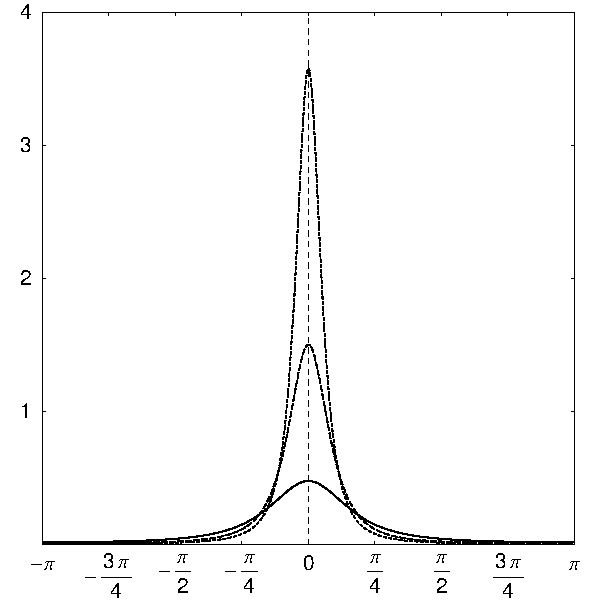
\includegraphics[width=0.7\textwidth]{images/poisson}
  \caption{The Poisson kernel $\fun{Q_{h}}{\cos\theta}$ for $h = 0.5,0.7,0.8$ and $\theta \in \interv{[}{-\pi}{\pi}{]}$.}
  \label{Basics:Figure:PoissonKernel}
\end{figure}

%\begin{figure}[htb]
%  \centering
%   \subfigure[$h=0.70$]
%     {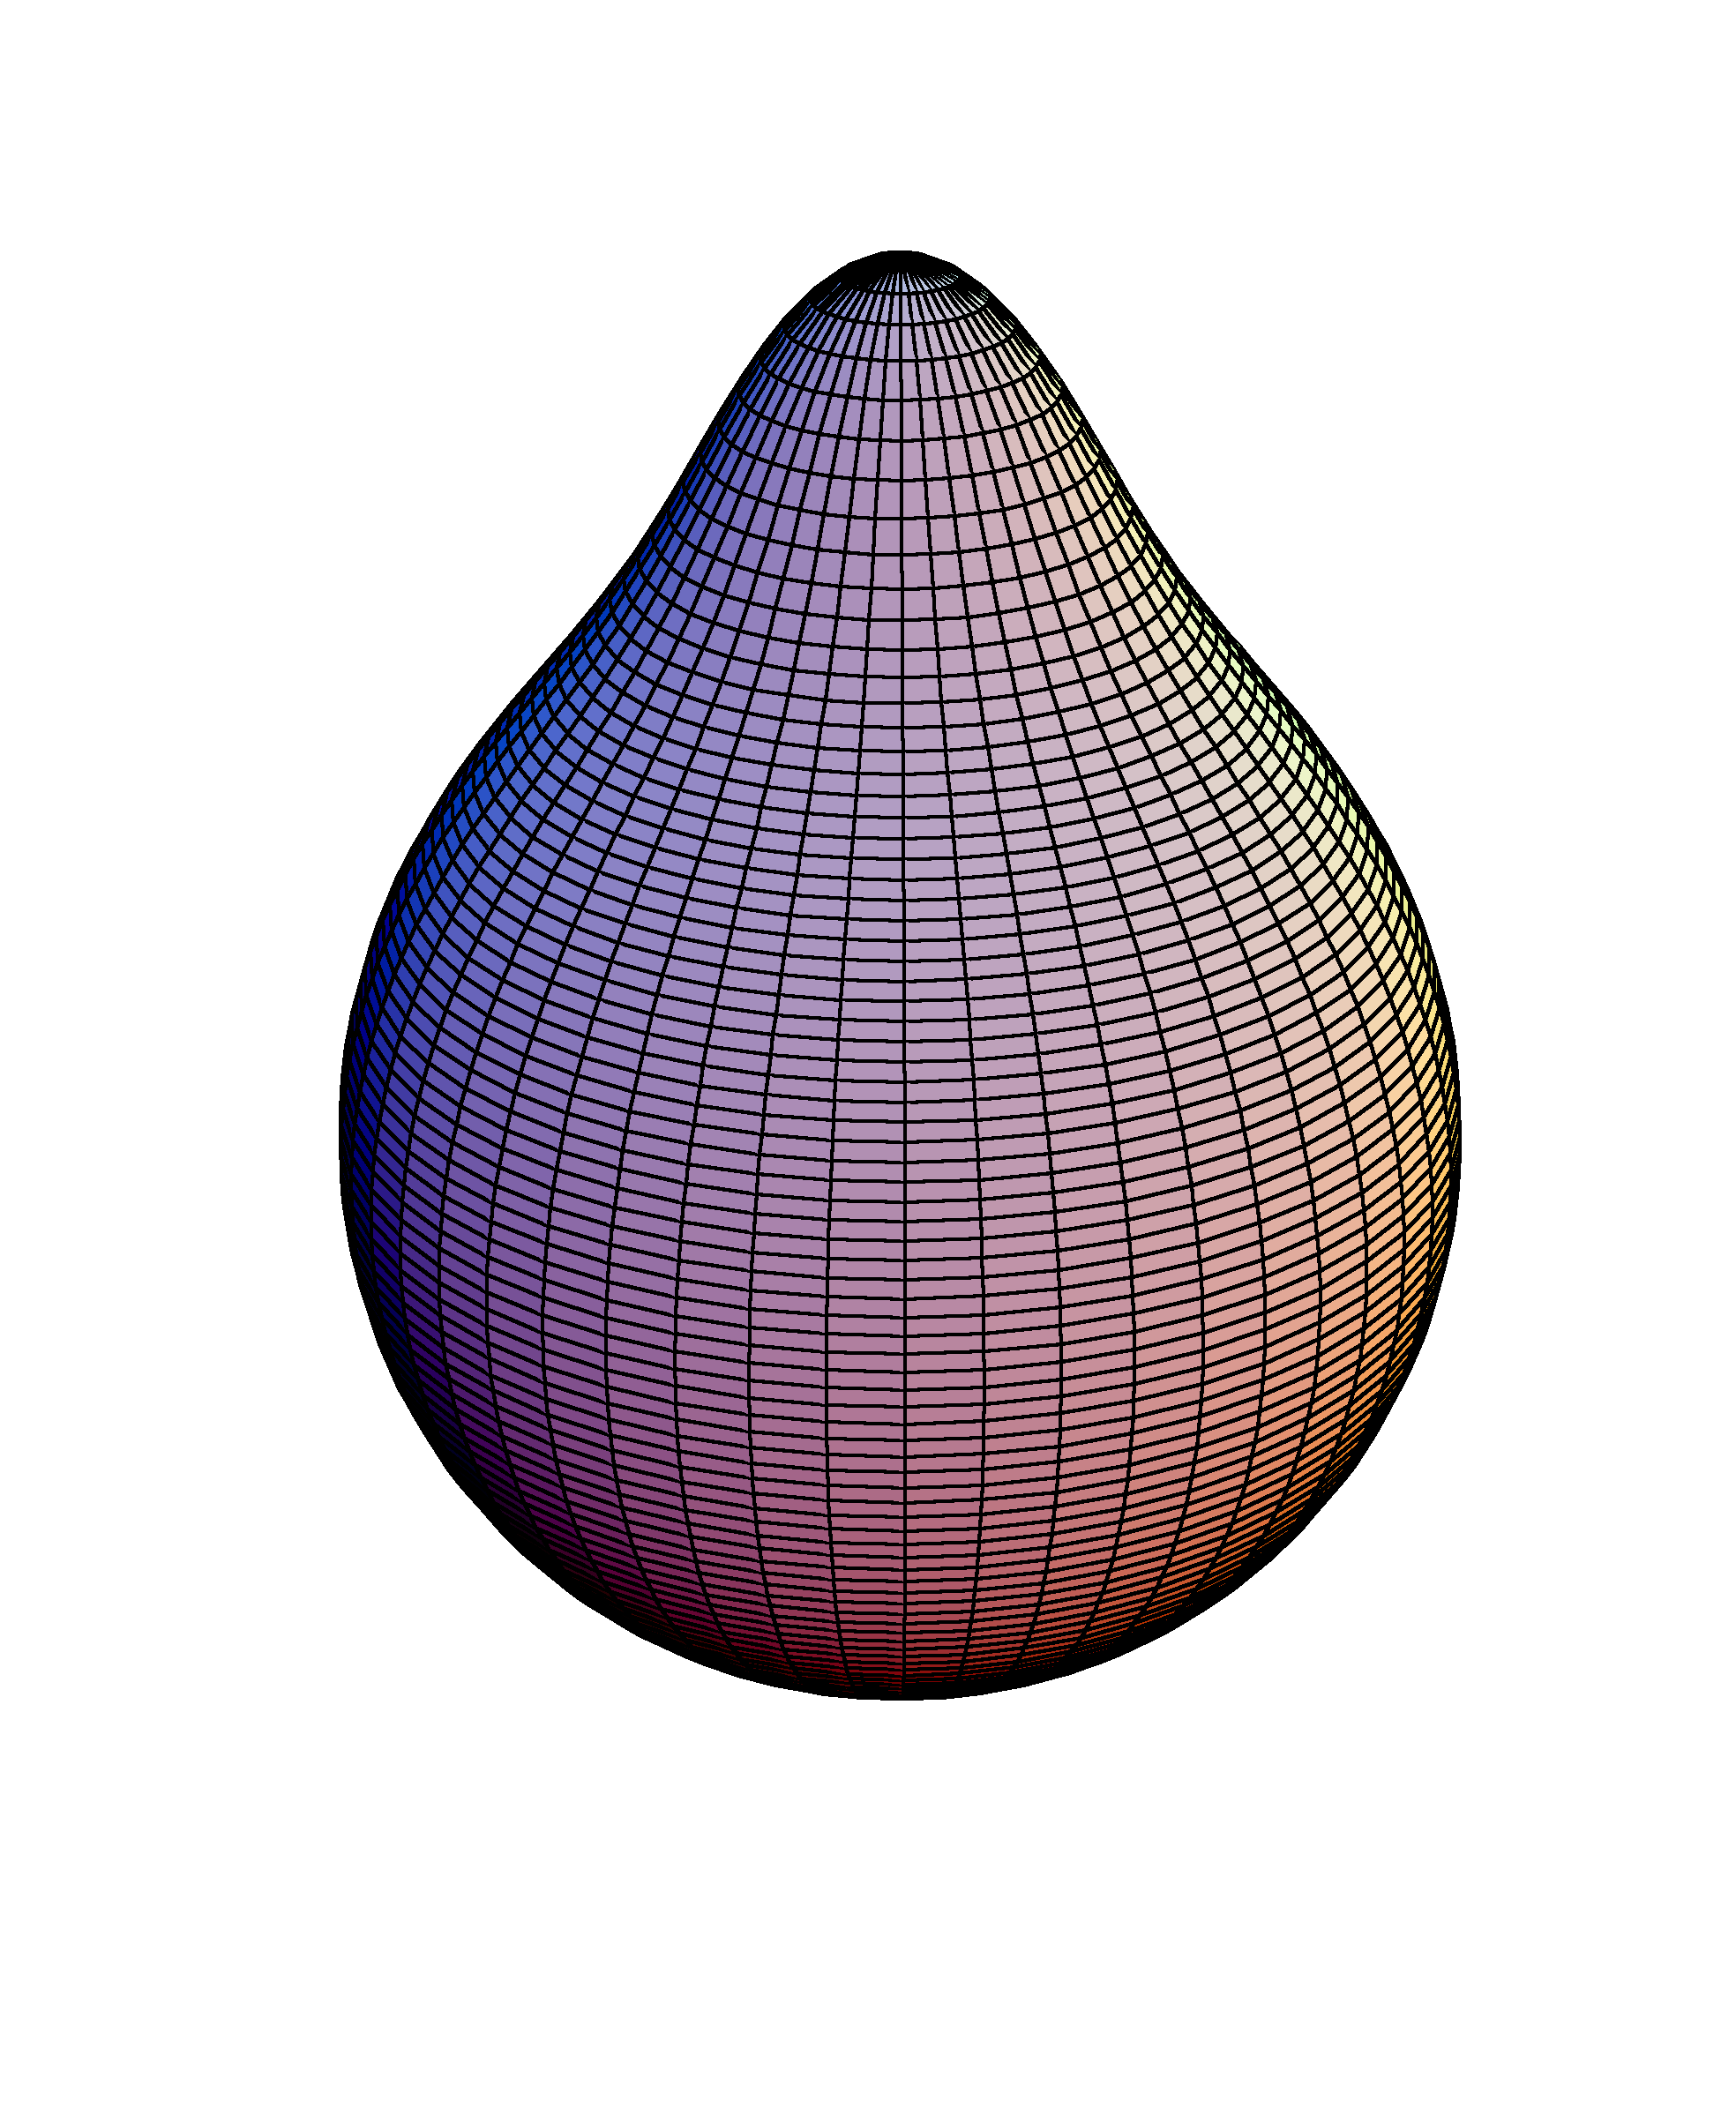
\includegraphics[width=0.5\textwidth]{images/p_070.png}}\hfill
%   \subfigure[$h=0.75$]
%     {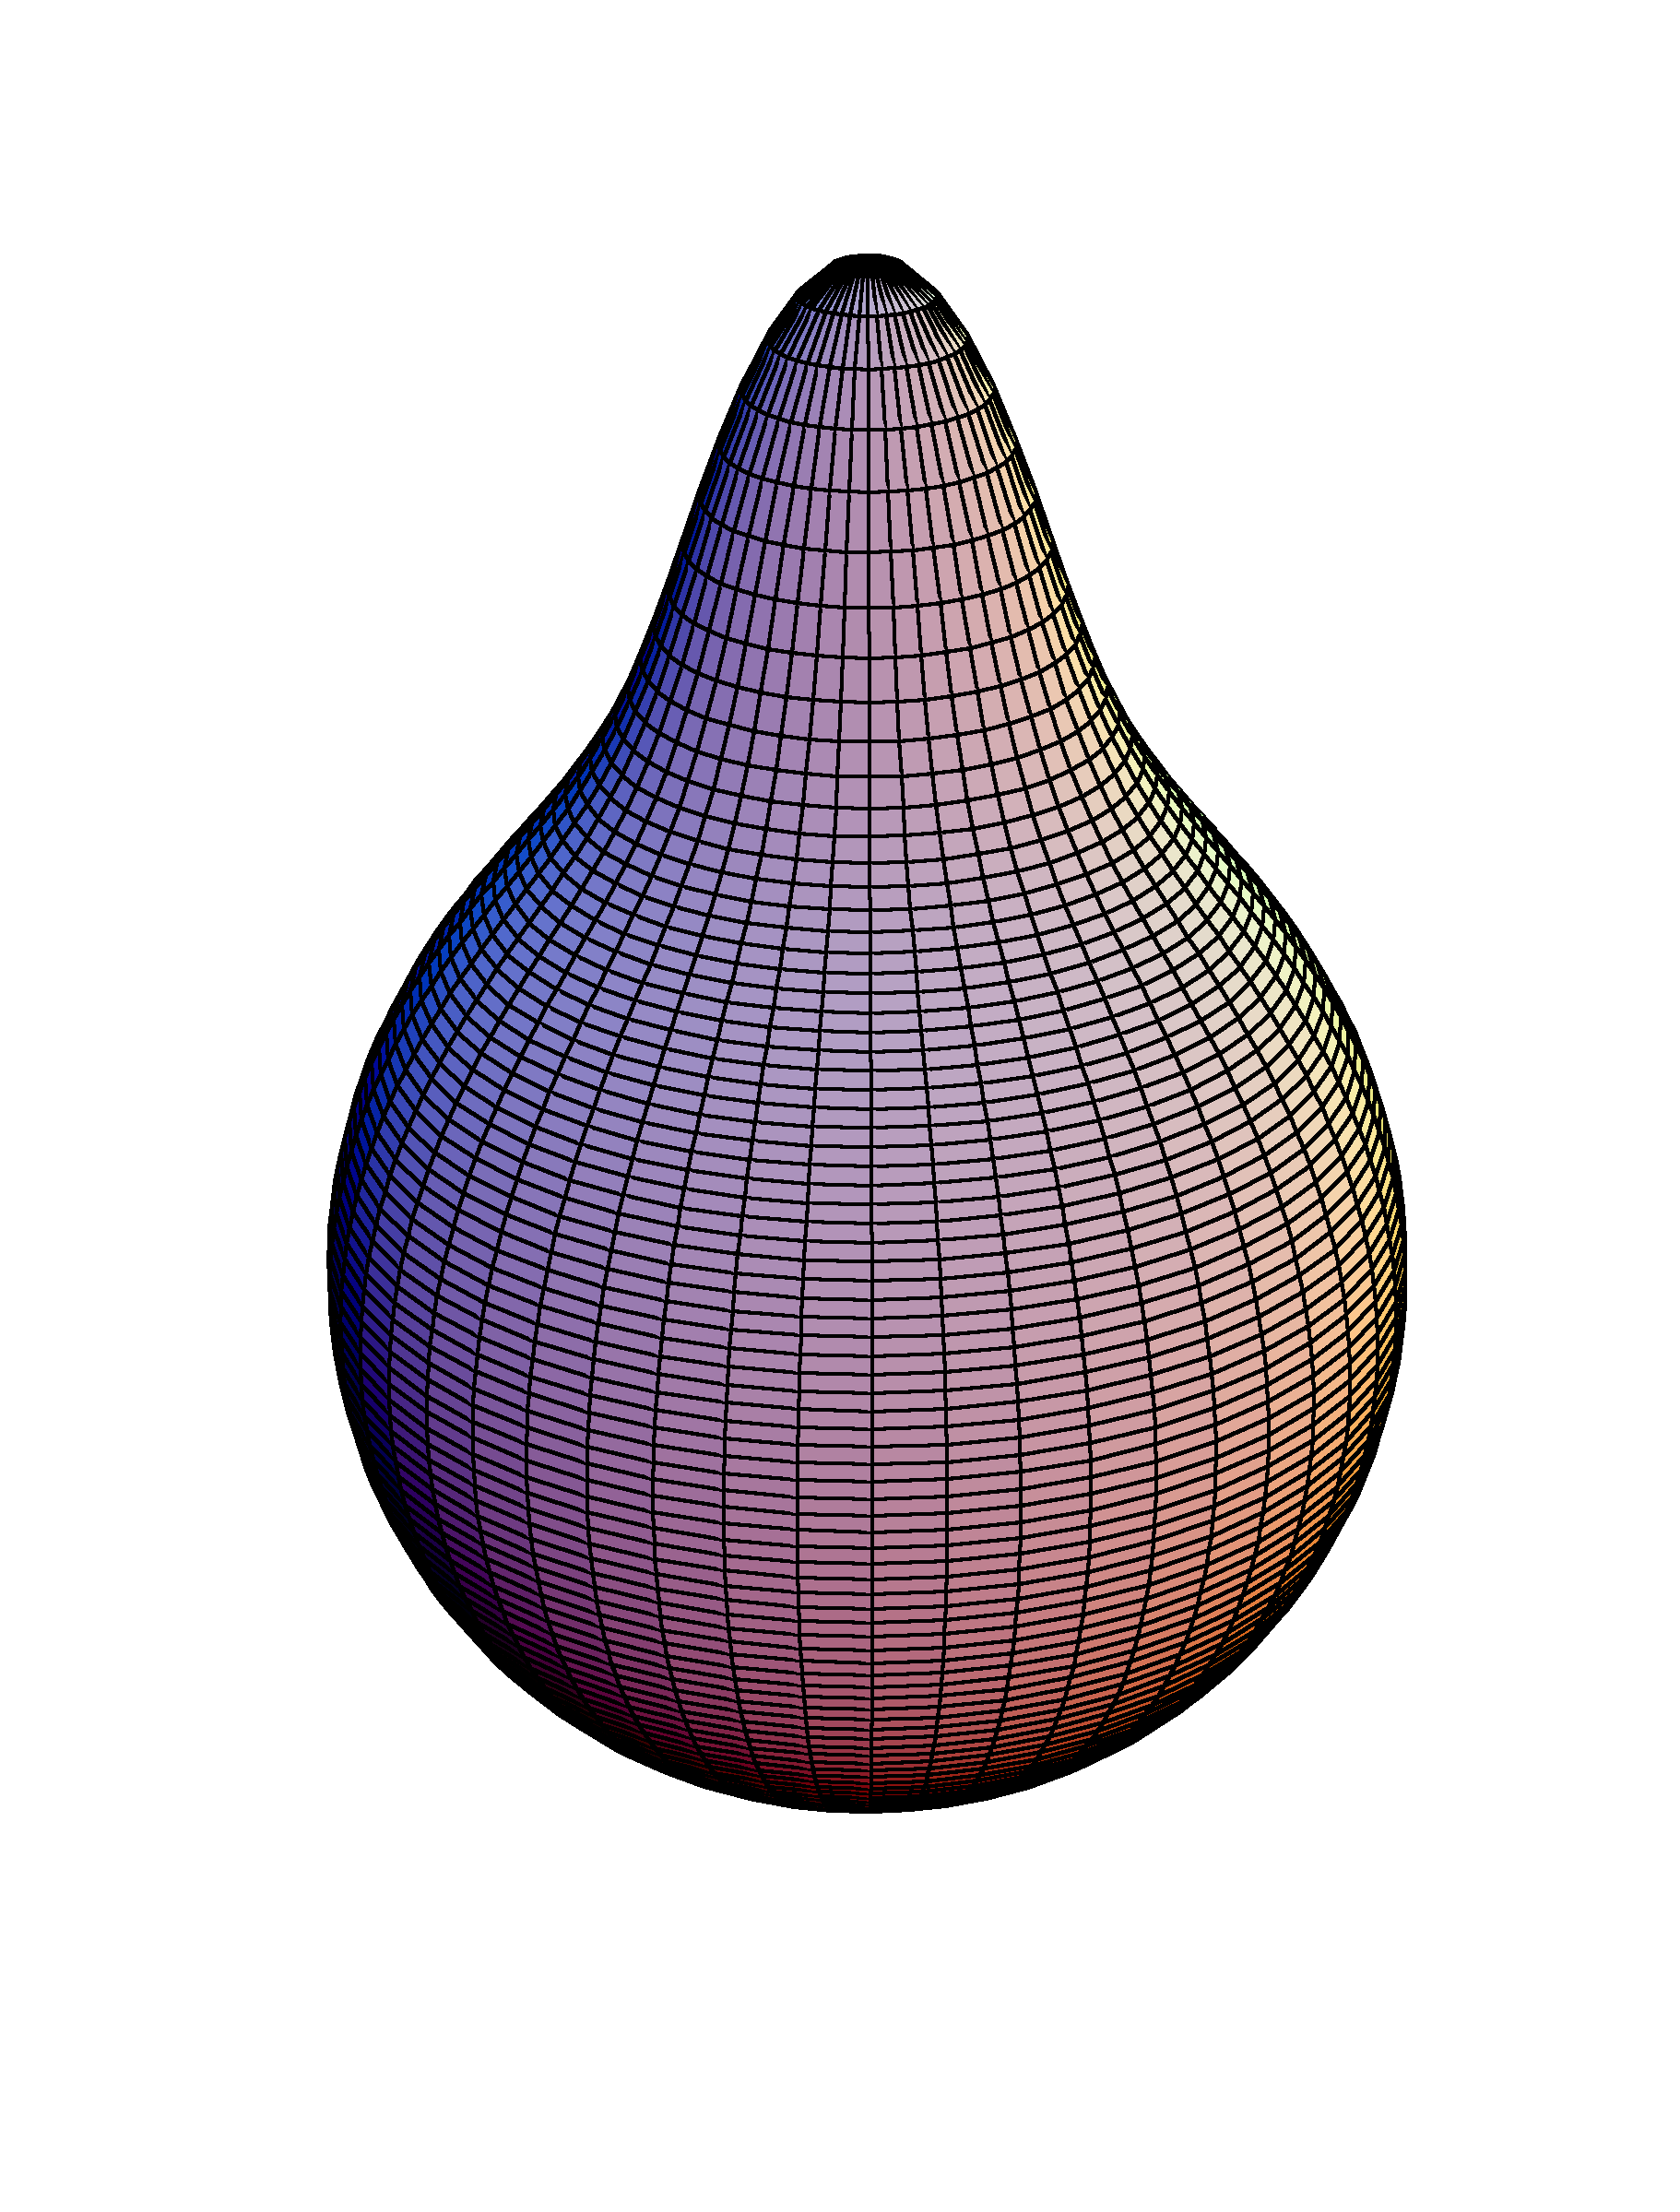
\includegraphics[width=0.5\textwidth]{images/p_075.png}}\\
%   \subfigure[$h=0.80$]
%     {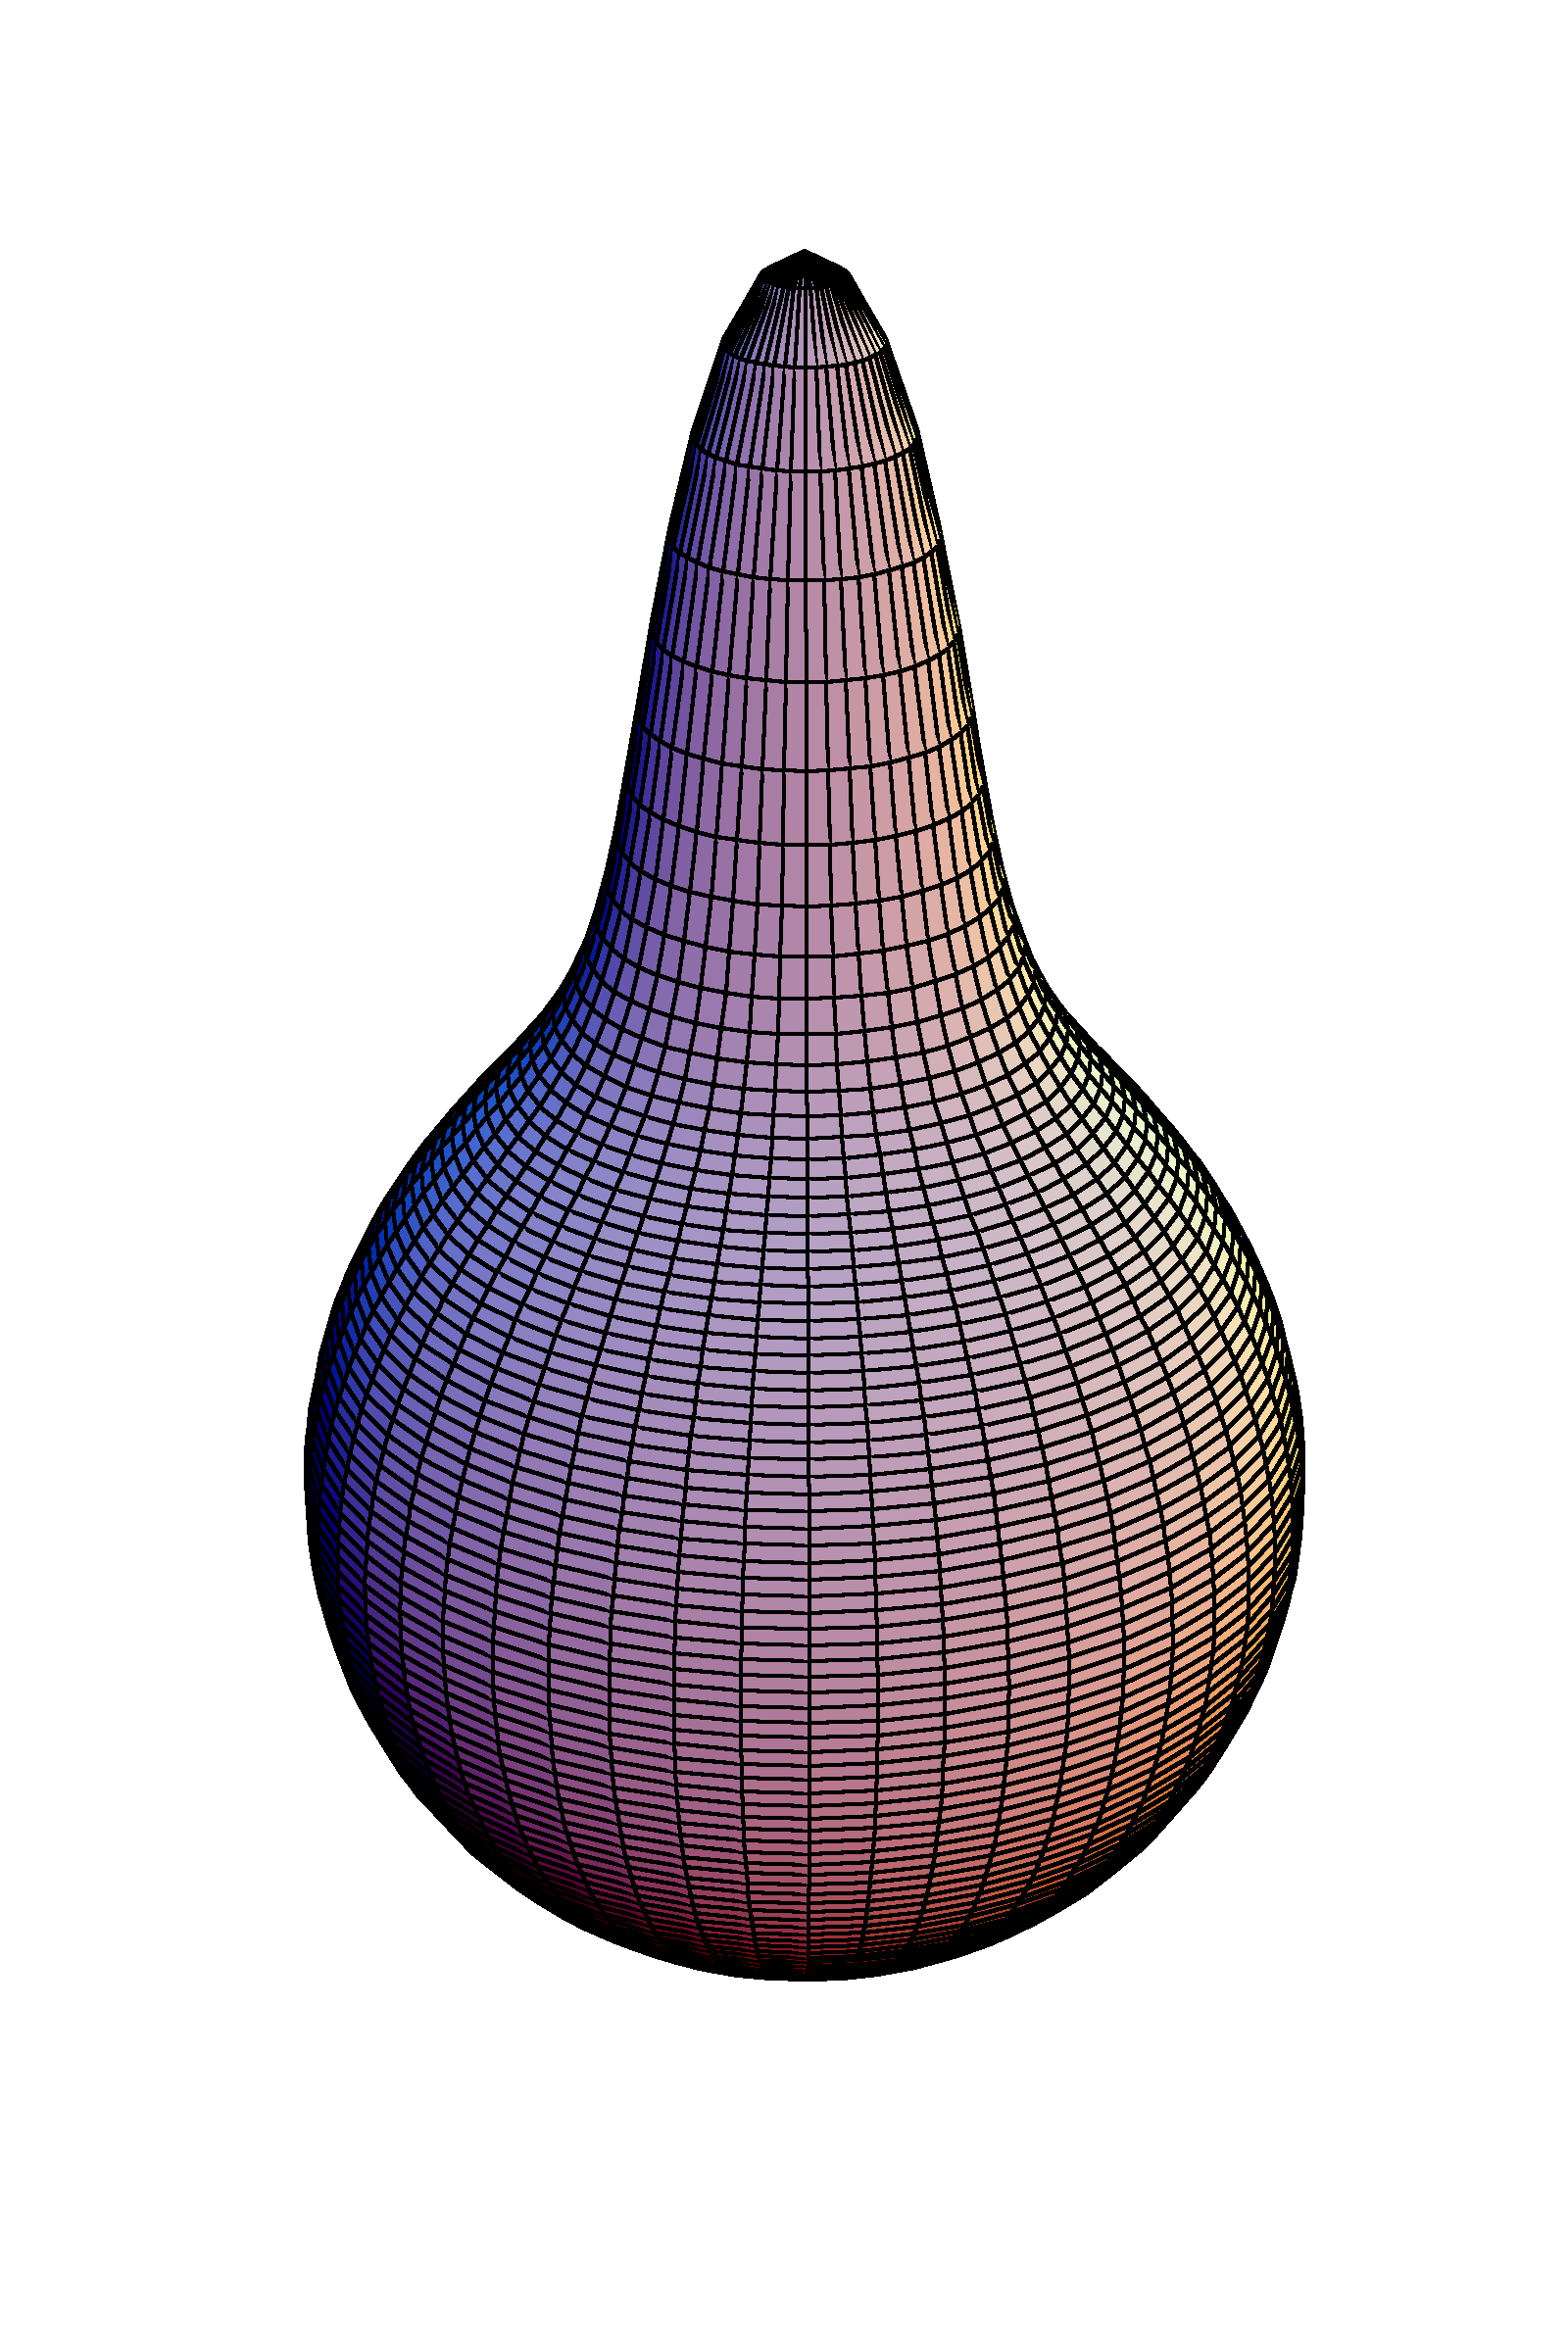
\includegraphics[width=0.5\textwidth]{images/p_080.png}}\hfill
%   \subfigure[$h=0.85$]
%     {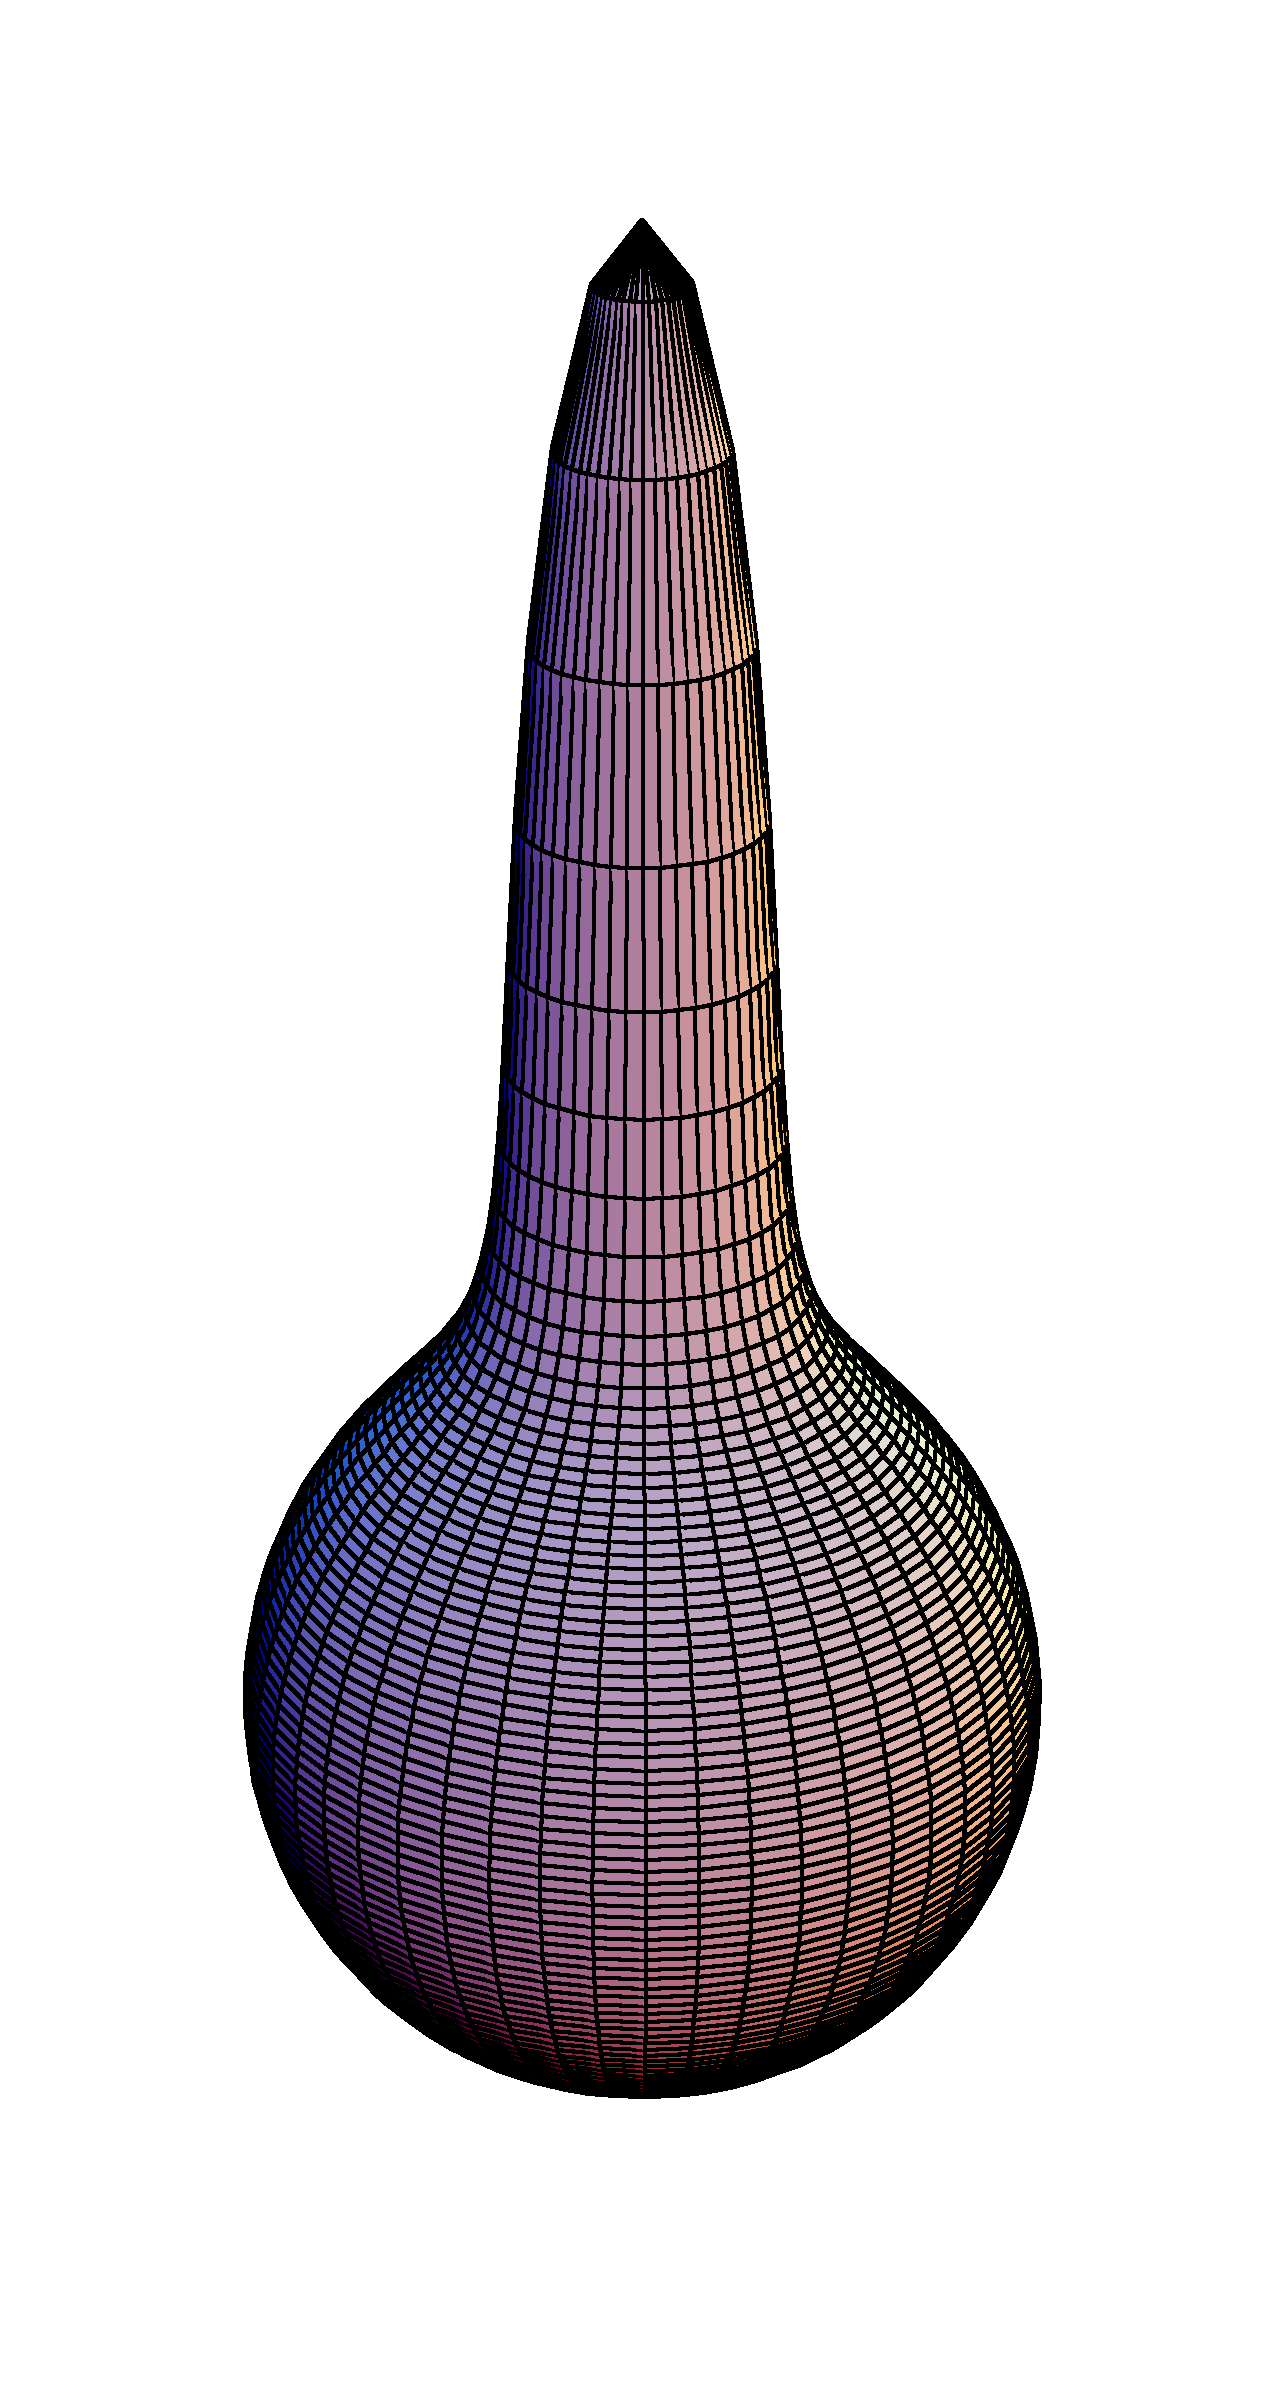
\includegraphics[width=0.5\textwidth]{images/p_085.png}}
%  \caption{The Poisson kernel plotted as a spherical radial basis function on the sphere for different values of $h$.}
%  \label{Basics:Figure:PoissonKernel2}
%\end{figure}

\begin{example}
  We define the \emph{singularity kernel} $S_{h}:\interv{[}{-1}{1}{]} \rightarrow \R$ by
  \[
    \fun{S_{h}}{x} := \frac{1}{2\pi} \frac{1}{\paren{1-2hx+h^2}^{1/2}}  \quad \paren{x \in \interv{[}{-1}{1}{]}}.
  \]
  Using \eqref{Basics:Solution} we obtain
  \[
    \fun{S_{h}}{x} = \sum_{k = 0}^{\infty} \frac{1}{2\pi} h^k \fun{P_k}{x}
  \]
  and therefore
  \[
    \fun{S_{h}^{\wedge}}{k} = \frac{2k+1}{2} h^k.
  \]
  See Figure \ref{Basics:Figure:SingularityKernel} and for more information \cite[pp. 112]{frgesc}.
\end{example}

\begin{figure}[tbp]
  \centering
  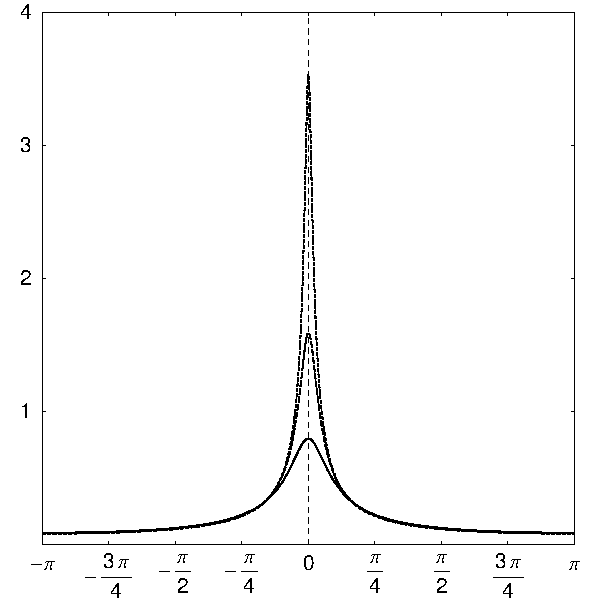
\includegraphics[width=0.7\textwidth]{images/singularity}
  \caption{The singularity kernel $\fun{S_{h}}{\cos\theta}$ for $h = 0.8,0.9,0.95$ and $\theta \in \interv{[}{-\pi}{\pi}{]}$.}
  \label{Basics:Figure:SingularityKernel}
\end{figure}

\begin{example}
  The \emph{Gauss-Weierstra� kernel} $W_{\rho}: \interv{[}{-\pi}{\pi}{]} \rightarrow \R$ is defined by
  \[
    \fun{W_{\rho}}{x} := \sum_{k=0}^{\infty} \e^{-k(k+1)\rho} \frac{2k+1}{4\pi} \fun{P_{k}}{x} \quad \paren{x \in \interv{[}{-1}{1}{]}}.
  \]
  Results due to Bochner (\cite{bochner1950},\cite{bochner1954}) assure $\fun{W_{\rho}}{x} \ge 0$ and we have
  \[
    \int_{\twosphere} \fun{W_{\rho}}{\V{\eta} \cdot \V{\xi}} \dx \V{\xi} = 1.
  \]
  For further properties we refer to \cite{frgesc} again. The kernel function $W_{\rho}$ is illustrated in Figure \ref{Basics:Figure:GaussWeierstrassKernel}.
\end{example}

\begin{figure}[tb]
  \centering
  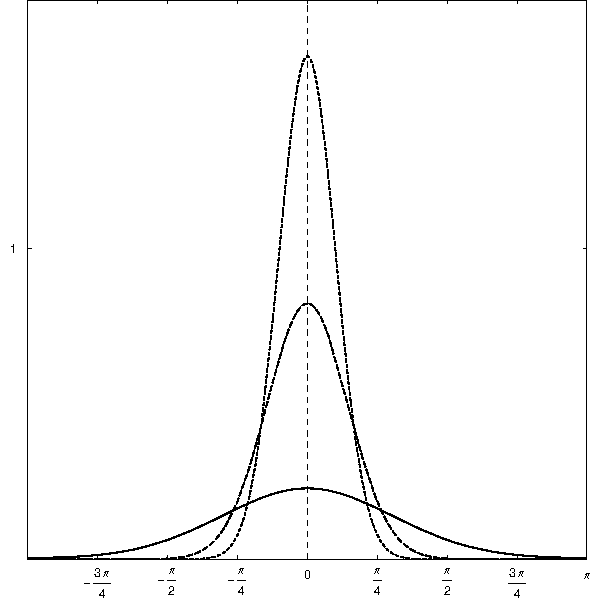
\includegraphics[width=0.7\textwidth]{images/gaussweierstrass}
  \caption{The Gauss-Weierstra� kernel $\fun{W_{\rho}}{\cos\theta}$ for $\rho = 0.4,0.1,0.05$ and $\theta \in \interv{[}{-\pi}{\pi}{]}$.}
  \label{Basics:Figure:GaussWeierstrassKernel}
\end{figure}

\begin{example}
  The locally supported kernel $L_{h,\lambda}: \interv{[}{-1}{1}{]} \rightarrow \R$ mentioned in \cite{frsc} and defined by
  \[
    \fun{L_{h,\lambda}}{x} := 
      \left\{\begin{array}{l@{\quad \text{if} \quad}l} 
                                              0 & -1 \le x \le h, \\
        \frac{\lambda+1}{2\pi(1-h)^{\lambda+1}}\paren{x-h}^{\lambda} &  h   < x \le 1,
      \end{array}\right.
  \]
  has the recursively defined symbol $\fun{L_{h,\lambda}^{\wedge}}{k}$ with
\begin{eqnarray*}
    \fun{L_{h,\lambda}^{\wedge}}{0} & = & 1,\\
    \paren{\lambda+1} \fun{L_{h,\lambda}^{\wedge}}{1} & = & \paren{\lambda + 1 + h},\\
    \paren{k+\lambda+2} \fun{L_{h,\lambda}^{\wedge}}{k+1} & = & \paren{2k+1} h \fun{L_{h,\lambda}^{\wedge}}{k} - \paren{k-\lambda-1} \fun{L_{h,\lambda}^{\wedge}}{k-1} 
    \quad \paren{k = 1,2,\ldots}.
\end{eqnarray*}
  Figure \ref{Basics:Figure:LKernel} shows the function $L_{h,\lambda}$ for different values $h$ and $\lambda$.
\end{example}

\begin{figure}[tb]
  \centering
   \subfigure[$\lambda=1.5$]
     {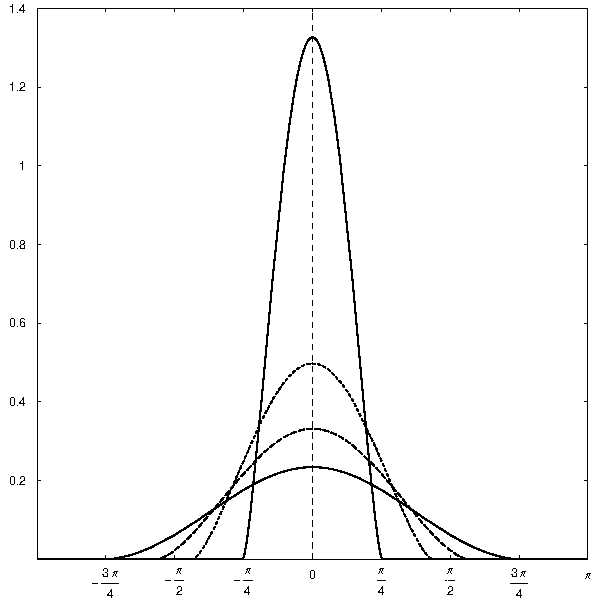
\includegraphics[width=0.33\textwidth]{images/locsup4}}\hfill
   \subfigure[$\lambda=1.0$]
     {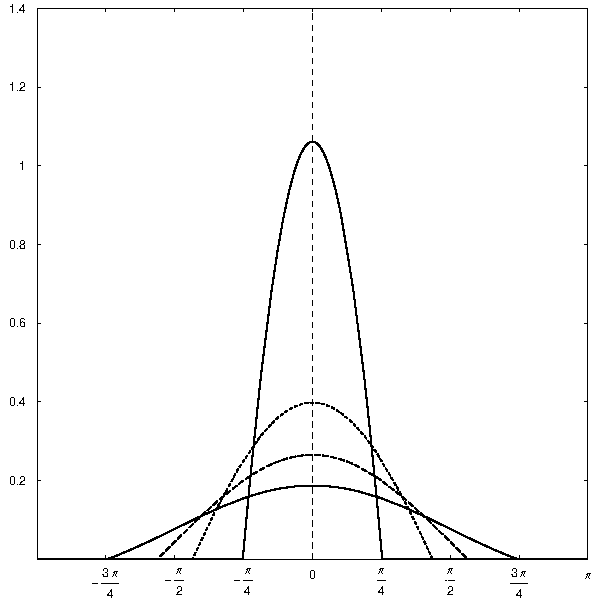
\includegraphics[width=0.33\textwidth]{images/locsup3}}\\
   \subfigure[$\lambda=0.5$]
     {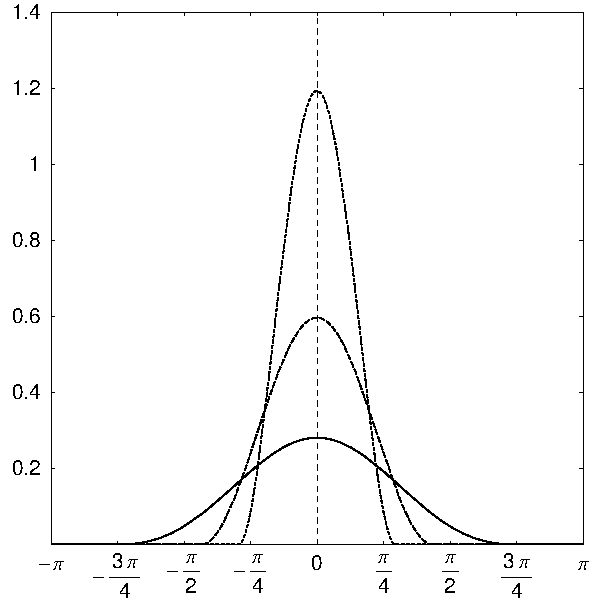
\includegraphics[width=0.33\textwidth]{images/locsup2}}\hfill
   \subfigure[$\lambda=0.2$]
     {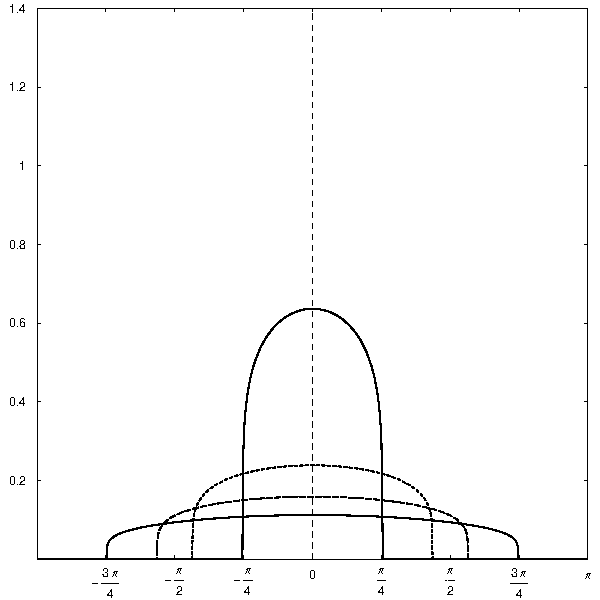
\includegraphics[width=0.33\textwidth]{images/locsup1}}
  \caption{The kernel $L_{h,\lambda}$ for $h = -0.7, -0.2, 0.2, 0.7$ and different values of $\lambda$.}
  \label{Basics:Figure:LKernel}
\end{figure}
\section{Spherical Radial Basis Functions}
\label{Basics:SphericalKernels}

\emph{Spherical radial basis basis functions} are the spherical counterpart of radial basis functions in Euclidean spaces. 
Generally, one starts with a function $K$ from $\Ln{2}{\interv{[}{-1}{1}{]}}$
%$: \interv{[}{-1}{1}{]} \rightarrow \C$ 
and defines for fixed $\V{\eta} \in \twosphere$ the $\V{\eta}$-zonal function 
\[
  \fun{K}{\V{\eta} \: \cdot}: \twosphere \rightarrow \C,\ \V{\xi} \mapsto \fun{K}{\V{\eta} \cdot \V{\xi}} \quad \paren{\V{\xi} \in \twosphere}.\] 
%by \[ \fun{K_{\V{\eta}}}{\V{\xi}} := \fun{G}{\V{\eta} \cdot \V{\xi}}.\]
By means of the \emph{Funk-Hecke formula} (see \cite[pp. 60]{frgesc}) we obtain for fixed $k \in \NZ$
\[
  \scalarproduct{\fun{K}{\V{\eta} \: \cdot}}{Y_{k}^n} = \int_{\twosphere} \fun{K}{\V{\eta} \cdot \V{\xi}} \overline{\fun{Y_{k}^n}{\V{\xi}}} \: \dx \V{\xi} = \fun{K^{\wedge}}{k} \overline{\fun{Y_{k}^n}{\V{\eta}}} \quad \paren{n=-k,\ldots,k},
\]
where the \emph{Legendre transform}, i.e. the \emph{symbol} of $K$, is given by
\[
  \fun{K^{\wedge}}{k} := 2 \pi \int_{-1}^{1} \fun{K}{x} \fun{P_{k}}{x} \dx x \quad \paren{k \in \NZ}.
\]
%We refer the interested reader to \cite{} and \cite{} for more details.
%The function $G$ can be developed into a series of Legendre polynomials
%\[ \fun{G}{x} = \sum_{k = 0}^{\infty} a_k \fun{P_k}{x}.\]
%where the coefficients $a_k$ are the scalar products
%\[ a_k = \scalarproduct{G}{P_{k}}_{\interv{[}{-1}{1}{]}} = \int_{-1}^{1} \fun{G}{x} \fun{P_k}{x} \dx x.\]
We have therefore 
\begin{equation}
  \label{Basics:Kernel}
  \fun{K}{\V{\eta} \cdot \V{\xi}} = \sum_{k = 0}^{\infty} \sum_{n=-k}^k \fun{K^{\wedge}}{k} \overline{\fun{Y_{k}^n}{\V{\eta}}} \fun{Y_{k}^n}{\V{\xi}} 
\end{equation}
and applying the Addition Theorem from Proposition \ref{Basics:AdditionTheorem}, we obtain for $K$ the orthogonal expansion
\begin{equation}
\label{Basics:OrthogonalKernelExpansion}
  \fun{K}{x} = \sum_{k = 0}^{\infty} \frac{2k+1}{4\pi} \fun{K^{\wedge}}{k} \fun{P_k}{x} \quad \paren{x \in \interv{[}{-1}{1}{]}}.
\end{equation}
%One is often interested in evaluating such an expansion on the sphere in a fast way when dealing with 
%spherical convolution. As an application of the algorithms developed in this text, one can derive 
%an algorithm based on the discrete spherical Fourier transform, as shown in Chapter \ref{}.

\begin{example}
We consider the generating series
\begin{equation}
  \label{Basics:GeneratingFunction}
  \fun{\phi}{h} := \sum_{k = 0}^{\infty} h^k \fun{P_k}{x} \quad \paren{x \in \interv{[}{-1}{1}{]}}
\end{equation}
which is absolutely and uniformly convergent for $h \in
\interv{(}{-1}{1}{)}$ with
\begin{equation}
  \label{Basics:Solution}
  \sum_{k = 0}^{\infty} h^k \fun{P_k}{x} = \frac{1}{\sqrt{1-2hx+h^2}}.
\end{equation}
This follows from the ordinary differential equation
\begin{equation}
\label{Basics:DifferentialEquation}
  \paren{1+h^2-2hx}\fun{\phi'}{h} = \paren{x-h}\fun{\phi}{h}
\end{equation}
obtained by differentiation with respect to $h$ and comparing coefficients in line with \eqref{Basics:GeneratingFunction}. Using the initial 
condition $\fun{\phi}{0}=1$ this yields the unique solution \eqref{Basics:Solution} of \eqref{Basics:DifferentialEquation}.
From this result, the identity
\begin{equation}
  \nonumber
  \sum_{k=0}^{\infty} \paren{2k+1} h^k \fun{P_k}{x} =
  \frac{1-h^2}{\paren{1-2hx+h^2}^{3/2}}
\end{equation}
 follows easily. When $h$ is restricted to $\interv{(}{0}{1}{)}$ the function
$Q_{h}:\interv{[}{-1}{1}{]} \rightarrow \R$, with
\begin{equation}
  \label{PoissonKernel}
  \nonumber
  \fun{Q_{h}}{x} := \frac{1}{4\pi} \frac{1-h^2}{\paren{1-2hx+h^2}^{3/2}} \quad \paren{x \in \interv{[}{-1}{1}{]}},
\end{equation}
is called \emph{Poisson kernel}. The symbol $\fun{Q_{h}^{\wedge}}{k}$ is given by 
\[
  \fun{Q_{h}^{\wedge}}{k} = h^k.
\]
We refer to Figure \ref{Basics:Figure:PoissonKernel} 
%and \ref{Basics:Figure:PoissonKernel2}
for a visual impression and mention that the parameter $h$
allows for controlling the concentration of the function's energy around
$x = 1$. The Poisson kernel is a positive function and normalized with
\[
  \int_{\twosphere} \fun{Q_{h}}{\V{\eta} \cdot \V{\xi}} \dx \V{\xi} = 1 \quad \paren{\V{\eta} \in \twosphere}.
\]
Further properties with respect to localization and smoothness are derived in \cite[pp. 112]{frgesc}.
\end{example}

\begin{figure}[tbp]
  \centering
  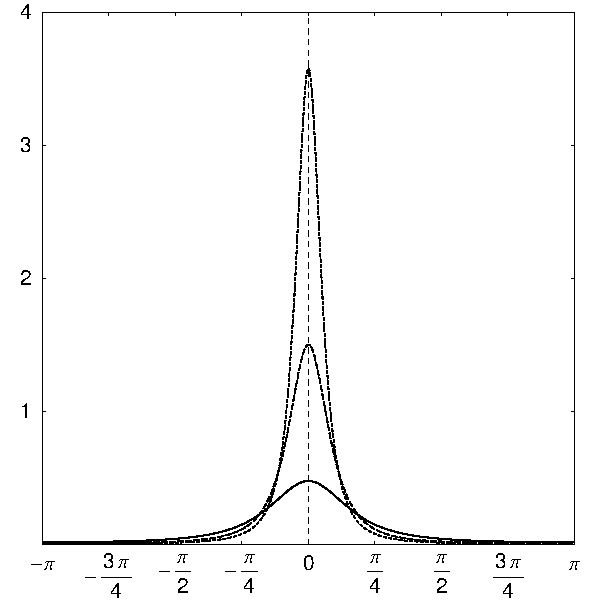
\includegraphics[width=0.7\textwidth]{images/poisson}
  \caption{The Poisson kernel $\fun{Q_{h}}{\cos\theta}$ for $h = 0.5,0.7,0.8$ and $\theta \in \interv{[}{-\pi}{\pi}{]}$.}
  \label{Basics:Figure:PoissonKernel}
\end{figure}

%\begin{figure}[htb]
%  \centering
%   \subfigure[$h=0.70$]
%     {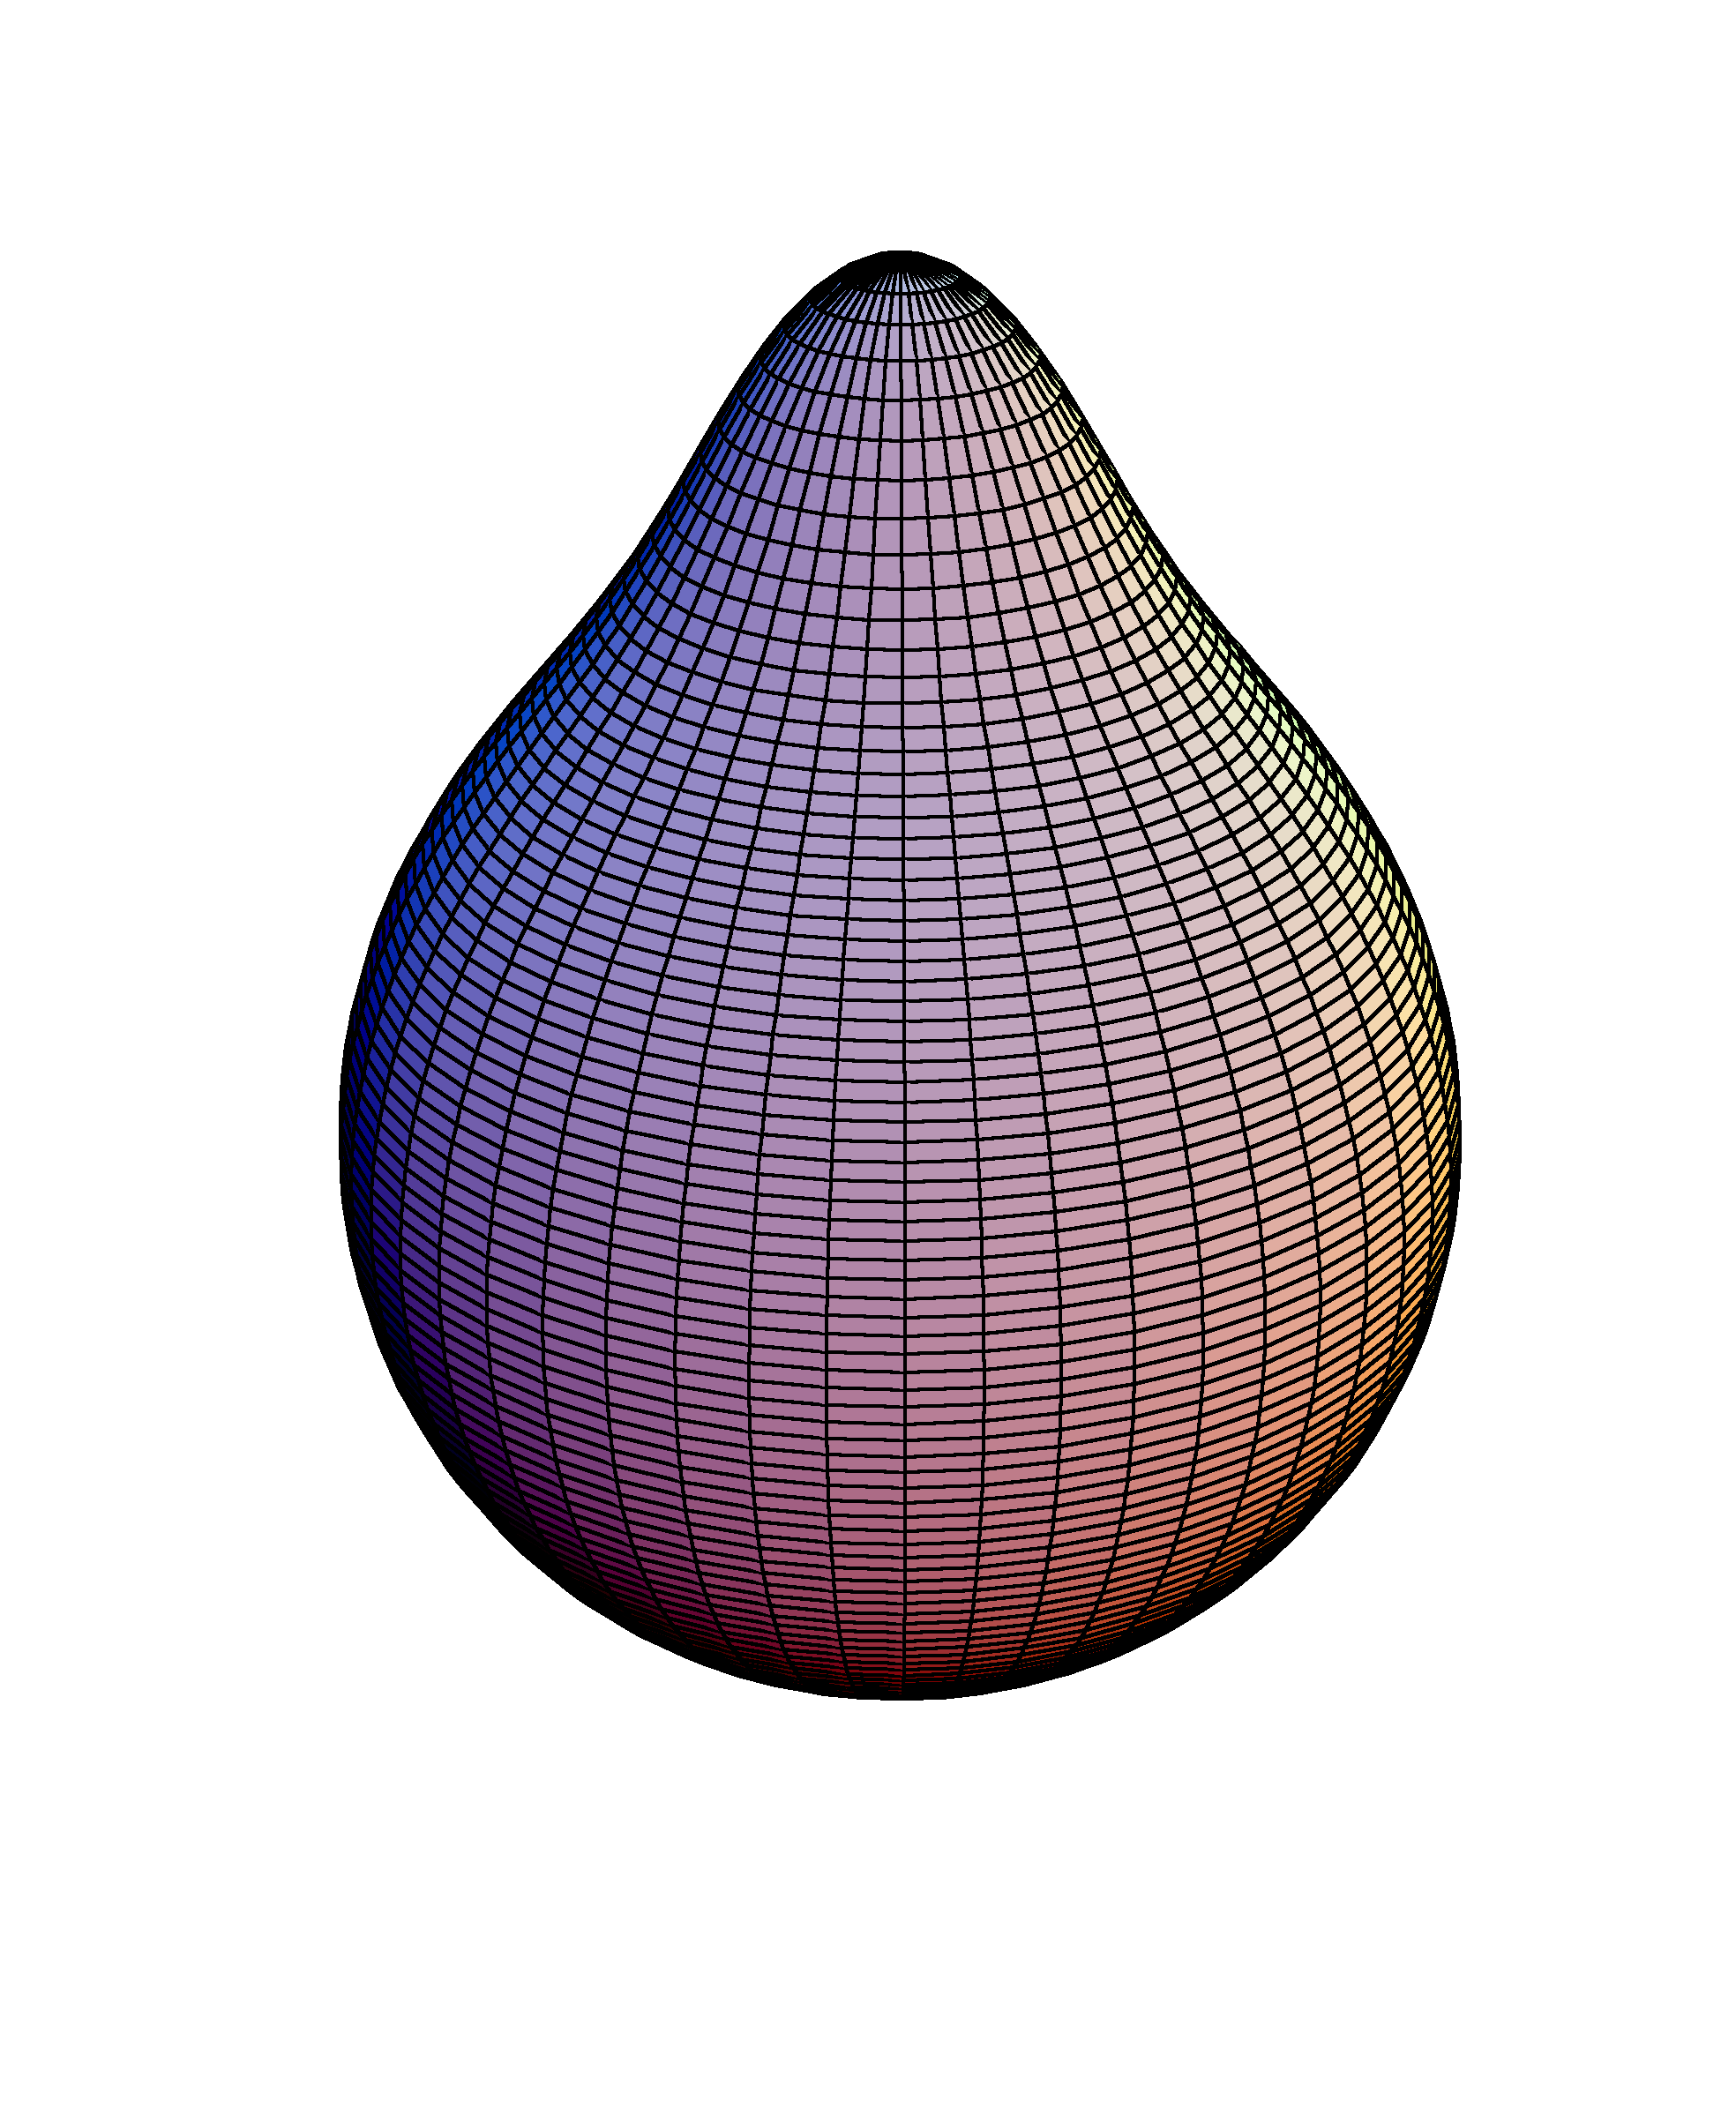
\includegraphics[width=0.5\textwidth]{images/p_070.png}}\hfill
%   \subfigure[$h=0.75$]
%     {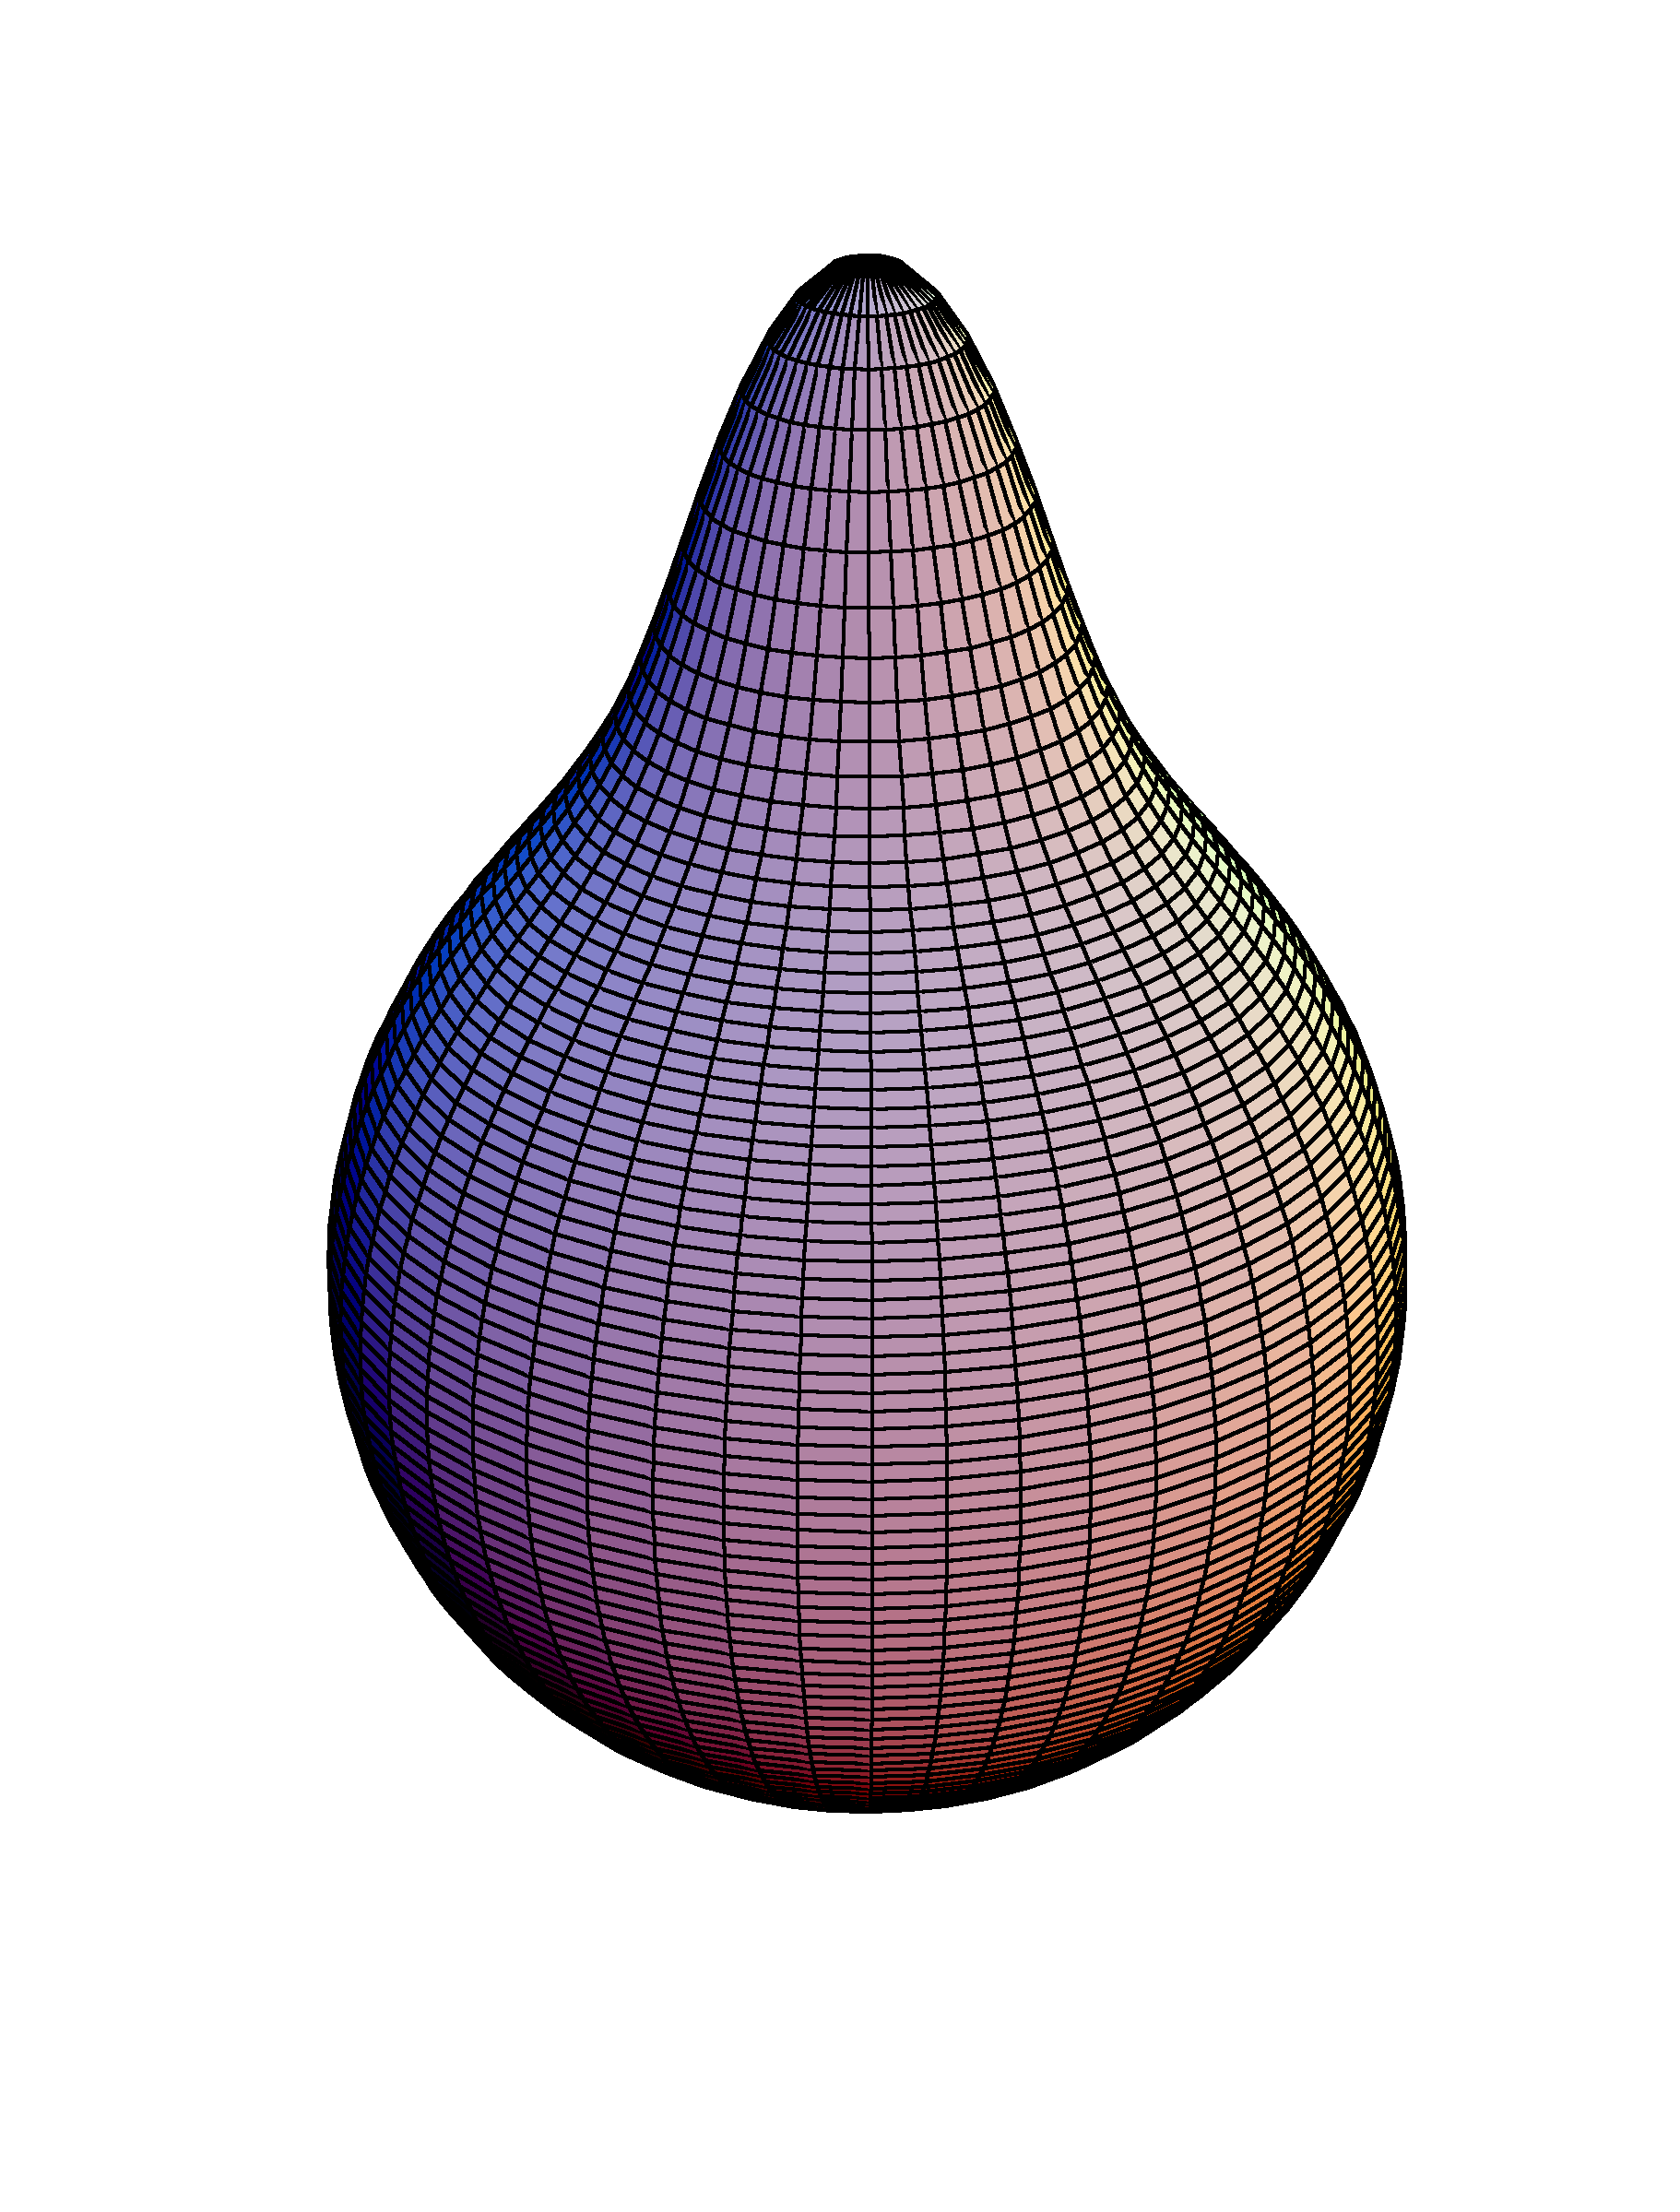
\includegraphics[width=0.5\textwidth]{images/p_075.png}}\\
%   \subfigure[$h=0.80$]
%     {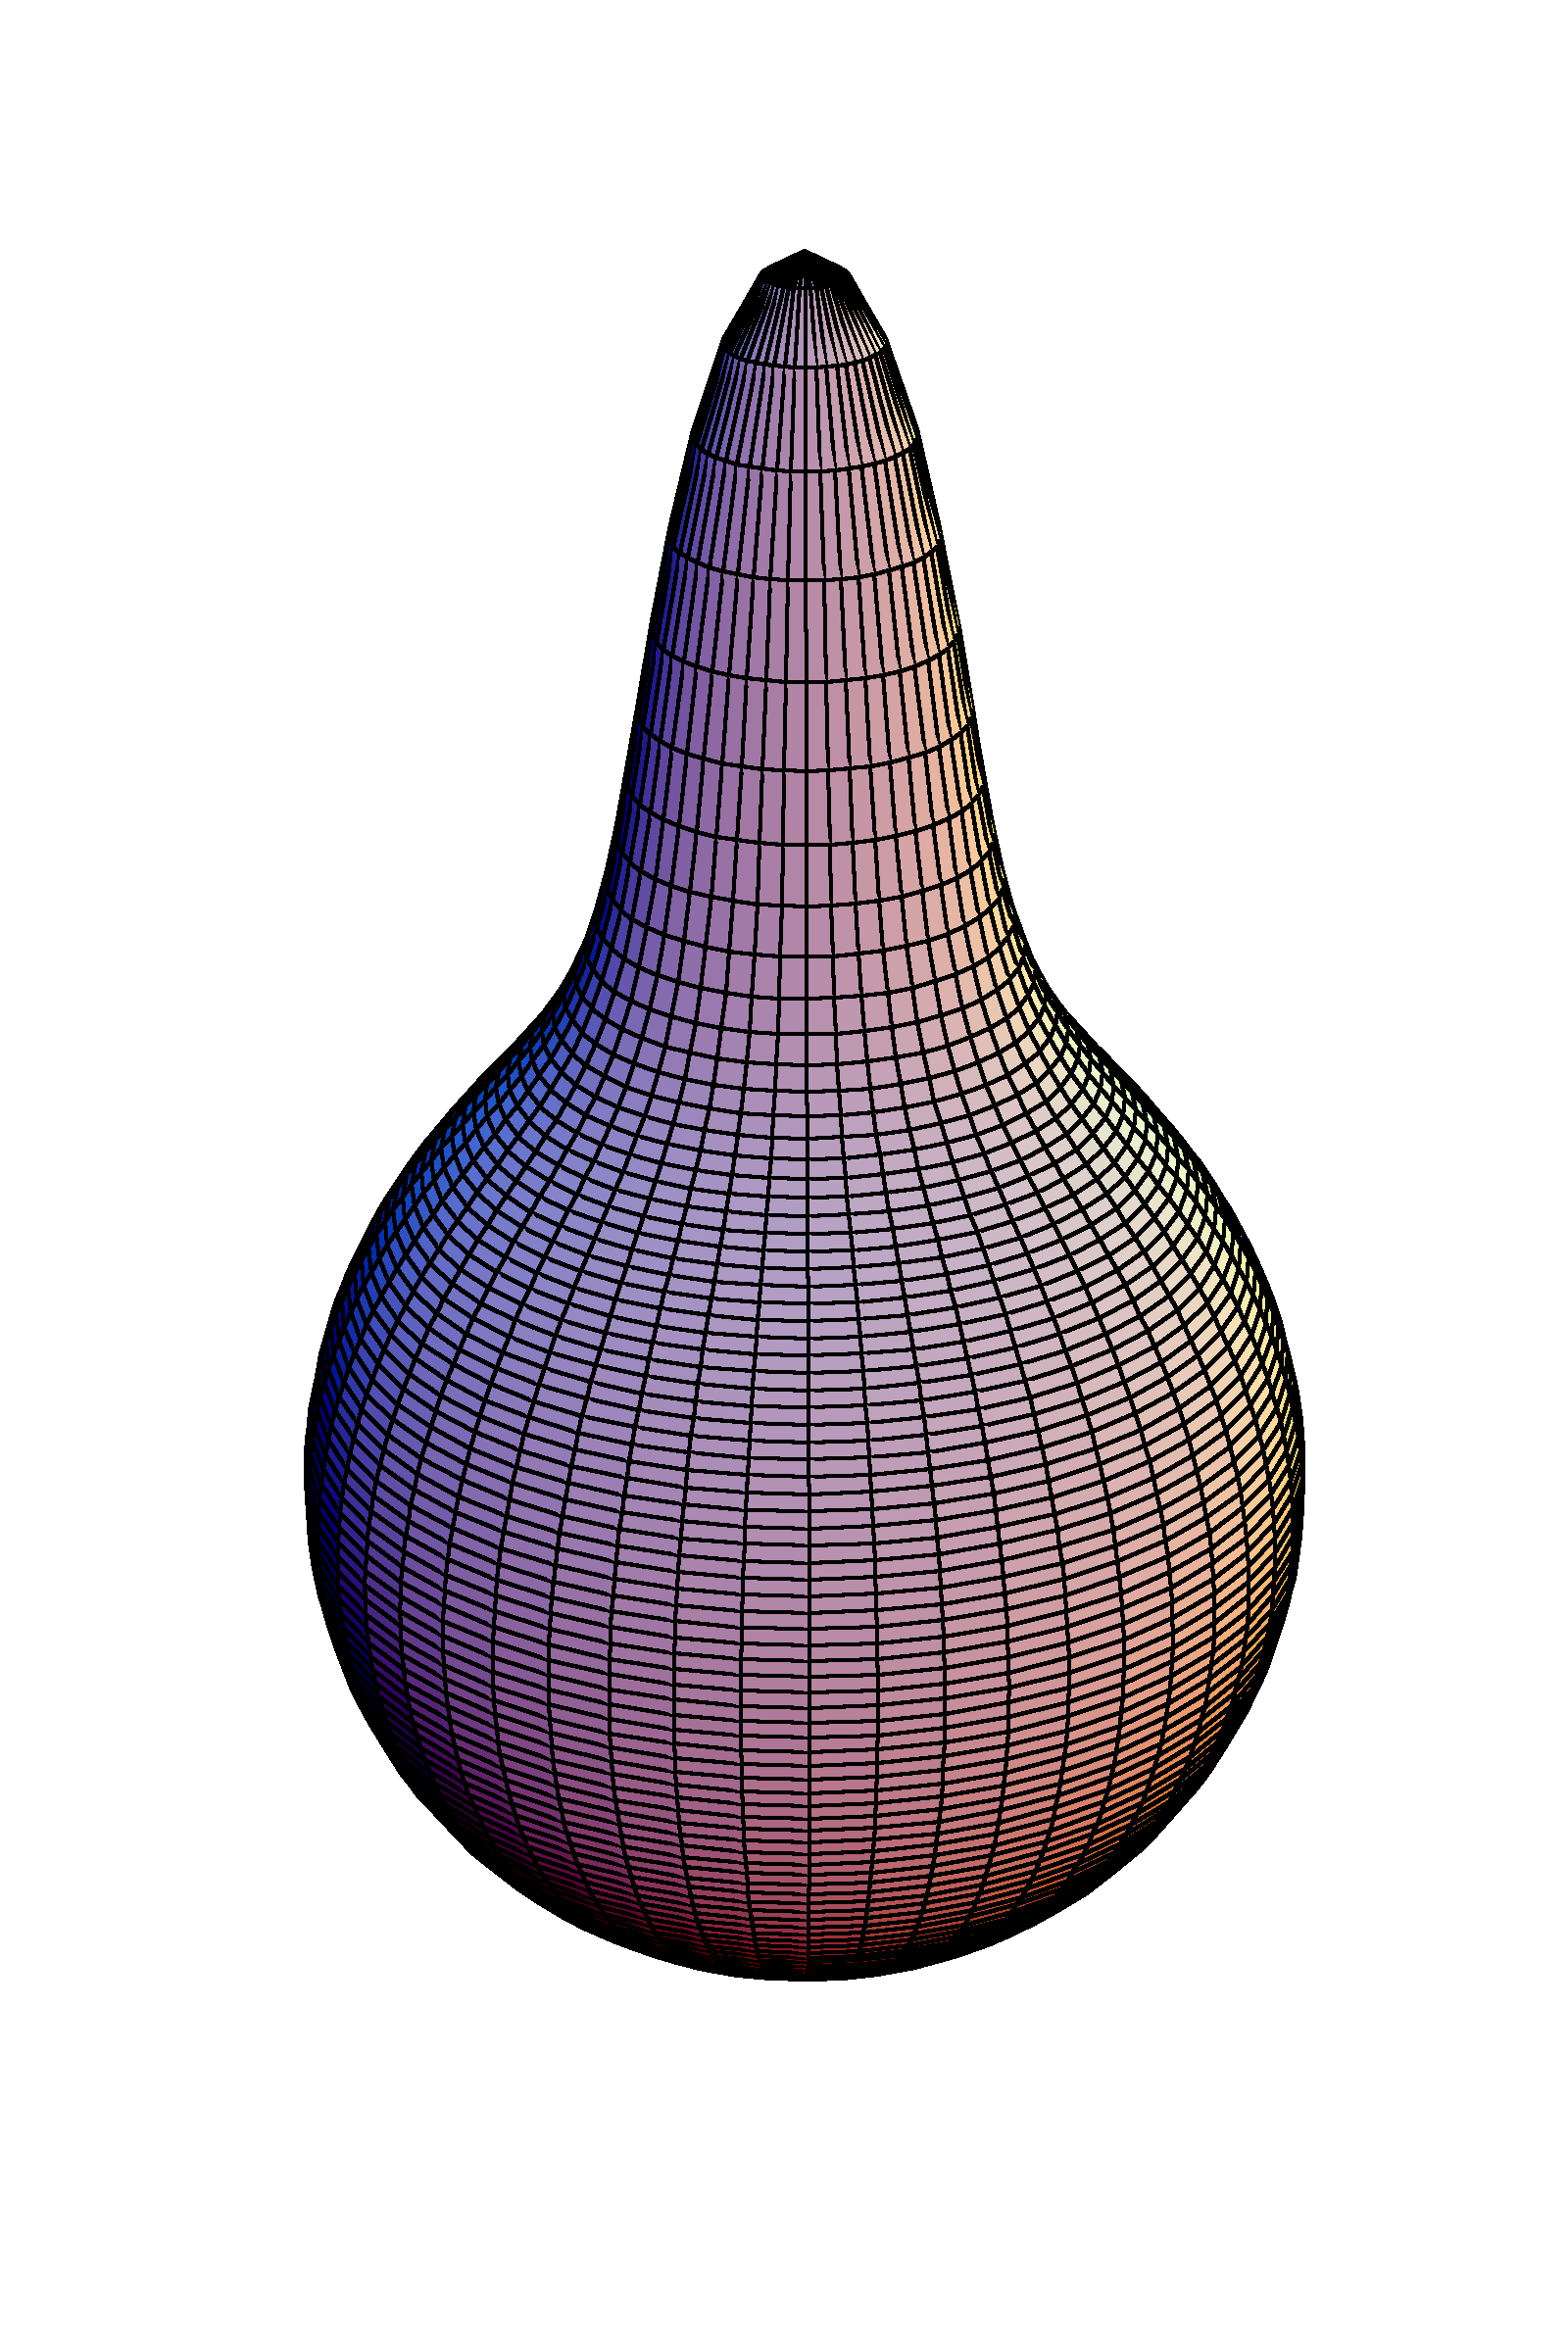
\includegraphics[width=0.5\textwidth]{images/p_080.png}}\hfill
%   \subfigure[$h=0.85$]
%     {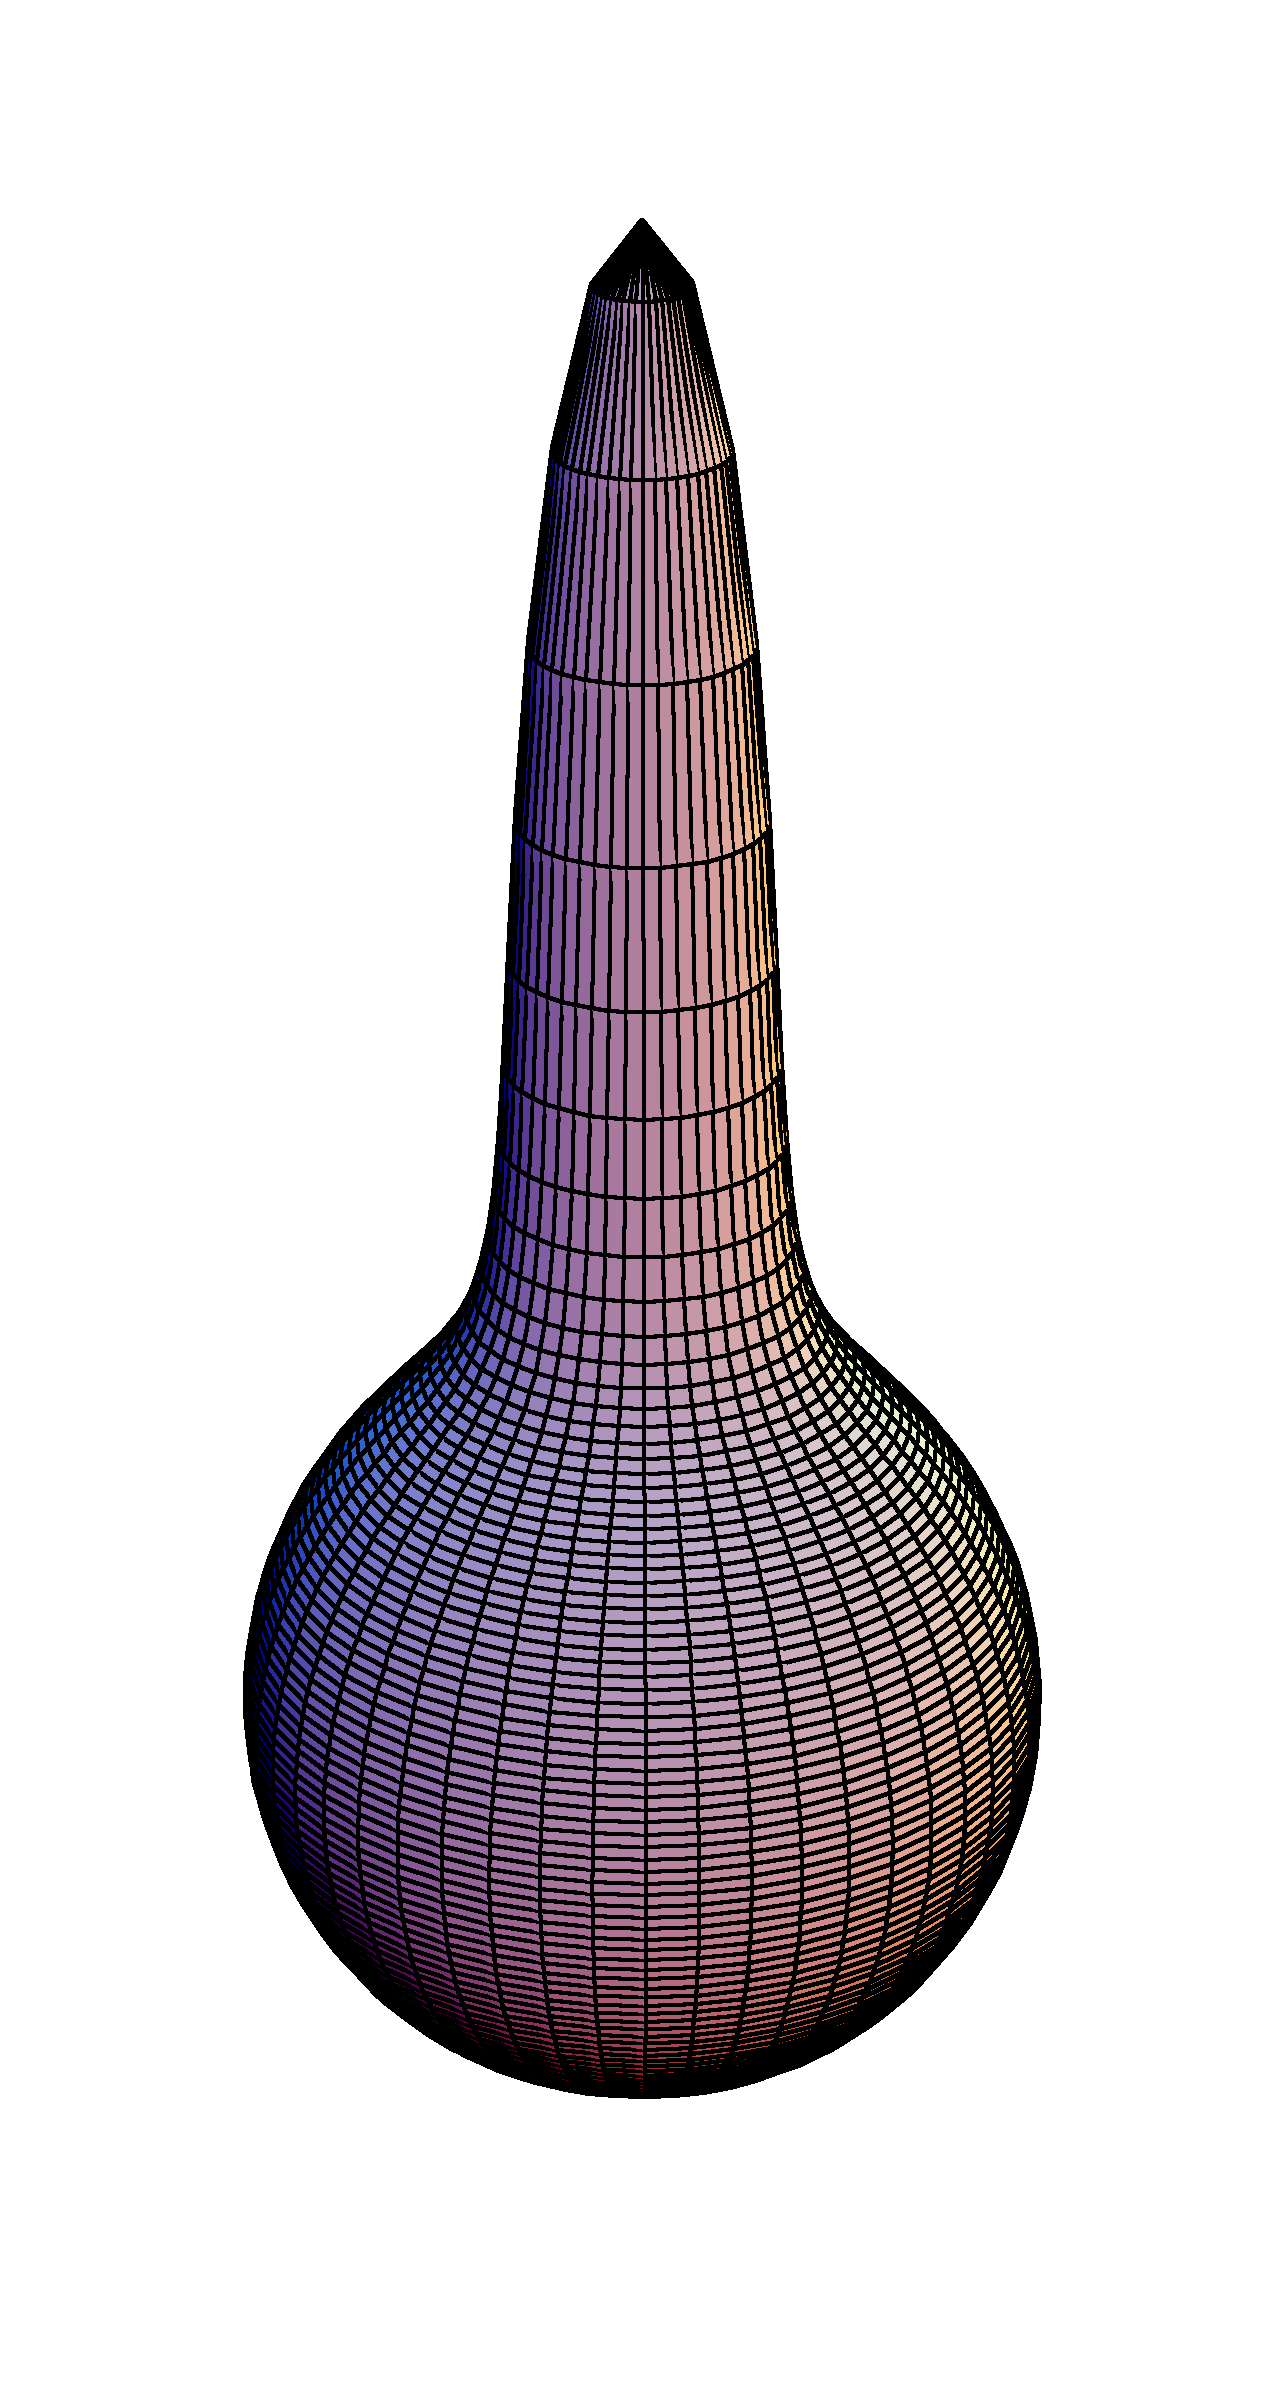
\includegraphics[width=0.5\textwidth]{images/p_085.png}}
%  \caption{The Poisson kernel plotted as a spherical radial basis function on the sphere for different values of $h$.}
%  \label{Basics:Figure:PoissonKernel2}
%\end{figure}

\begin{example}
  We define the \emph{singularity kernel} $S_{h}:\interv{[}{-1}{1}{]} \rightarrow \R$ by
  \[
    \fun{S_{h}}{x} := \frac{1}{2\pi} \frac{1}{\paren{1-2hx+h^2}^{1/2}}  \quad \paren{x \in \interv{[}{-1}{1}{]}}.
  \]
  Using \eqref{Basics:Solution} we obtain
  \[
    \fun{S_{h}}{x} = \sum_{k = 0}^{\infty} \frac{1}{2\pi} h^k \fun{P_k}{x}
  \]
  and therefore
  \[
    \fun{S_{h}^{\wedge}}{k} = \frac{2k+1}{2} h^k.
  \]
  See Figure \ref{Basics:Figure:SingularityKernel} and for more information \cite[pp. 112]{frgesc}.
\end{example}

\begin{figure}[tbp]
  \centering
  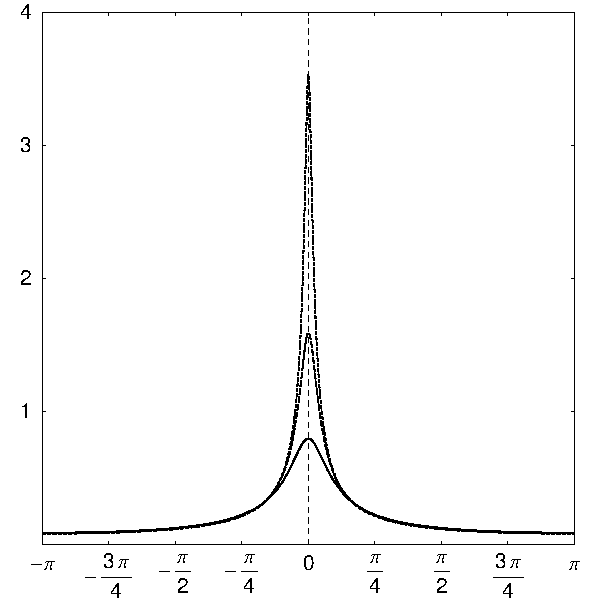
\includegraphics[width=0.7\textwidth]{images/singularity}
  \caption{The singularity kernel $\fun{S_{h}}{\cos\theta}$ for $h = 0.8,0.9,0.95$ and $\theta \in \interv{[}{-\pi}{\pi}{]}$.}
  \label{Basics:Figure:SingularityKernel}
\end{figure}

\begin{example}
  The \emph{Gauss-Weierstra� kernel} $W_{\rho}: \interv{[}{-\pi}{\pi}{]} \rightarrow \R$ is defined by
  \[
    \fun{W_{\rho}}{x} := \sum_{k=0}^{\infty} \e^{-k(k+1)\rho} \frac{2k+1}{4\pi} \fun{P_{k}}{x} \quad \paren{x \in \interv{[}{-1}{1}{]}}.
  \]
  Results due to Bochner (\cite{bochner1950},\cite{bochner1954}) assure $\fun{W_{\rho}}{x} \ge 0$ and we have
  \[
    \int_{\twosphere} \fun{W_{\rho}}{\V{\eta} \cdot \V{\xi}} \dx \V{\xi} = 1.
  \]
  For further properties we refer to \cite{frgesc} again. The kernel function $W_{\rho}$ is illustrated in Figure \ref{Basics:Figure:GaussWeierstrassKernel}.
\end{example}

\begin{figure}[tb]
  \centering
  \includegraphics[width=0.7\textwidth]{images/gaussweierstrass}
  \caption{The Gauss-Weierstra� kernel $\fun{W_{\rho}}{\cos\theta}$ for $\rho = 0.4,0.1,0.05$ and $\theta \in \interv{[}{-\pi}{\pi}{]}$.}
  \label{Basics:Figure:GaussWeierstrassKernel}
\end{figure}

\begin{example}
  The locally supported kernel $L_{h,\lambda}: \interv{[}{-1}{1}{]} \rightarrow \R$ mentioned in \cite{frsc} and defined by
  \[
    \fun{L_{h,\lambda}}{x} := 
      \left\{\begin{array}{l@{\quad \text{if} \quad}l} 
                                              0 & -1 \le x \le h, \\
        \frac{\lambda+1}{2\pi(1-h)^{\lambda+1}}\paren{x-h}^{\lambda} &  h   < x \le 1,
      \end{array}\right.
  \]
  has the recursively defined symbol $\fun{L_{h,\lambda}^{\wedge}}{k}$ with
\begin{eqnarray*}
    \fun{L_{h,\lambda}^{\wedge}}{0} & = & 1,\\
    \paren{\lambda+1} \fun{L_{h,\lambda}^{\wedge}}{1} & = & \paren{\lambda + 1 + h},\\
    \paren{k+\lambda+2} \fun{L_{h,\lambda}^{\wedge}}{k+1} & = & \paren{2k+1} h \fun{L_{h,\lambda}^{\wedge}}{k} - \paren{k-\lambda-1} \fun{L_{h,\lambda}^{\wedge}}{k-1} 
    \quad \paren{k = 1,2,\ldots}.
\end{eqnarray*}
  Figure \ref{Basics:Figure:LKernel} shows the function $L_{h,\lambda}$ for different values $h$ and $\lambda$.
\end{example}

\begin{figure}[tb]
  \centering
   \subfigure[$\lambda=1.5$]
     {\includegraphics[width=0.33\textwidth]{images/locsup4}}\hfill
   \subfigure[$\lambda=1.0$]
     {\includegraphics[width=0.33\textwidth]{images/locsup3}}\\
   \subfigure[$\lambda=0.5$]
     {\includegraphics[width=0.33\textwidth]{images/locsup2}}\hfill
   \subfigure[$\lambda=0.2$]
     {\includegraphics[width=0.33\textwidth]{images/locsup1}}
  \caption{The kernel $L_{h,\lambda}$ for $h = -0.7, -0.2, 0.2, 0.7$ and different values of $\lambda$.}
  \label{Basics:Figure:LKernel}
\end{figure}
\section{Spherical Radial Basis Functions}
\label{Basics:SphericalKernels}

\emph{Spherical radial basis basis functions} are the spherical counterpart of radial basis functions in Euclidean spaces. 
Generally, one starts with a function $K$ from $\Ln{2}{\interv{[}{-1}{1}{]}}$
%$: \interv{[}{-1}{1}{]} \rightarrow \C$ 
and defines for fixed $\V{\eta} \in \twosphere$ the $\V{\eta}$-zonal function 
\[
  \fun{K}{\V{\eta} \: \cdot}: \twosphere \rightarrow \C,\ \V{\xi} \mapsto \fun{K}{\V{\eta} \cdot \V{\xi}} \quad \paren{\V{\xi} \in \twosphere}.\] 
%by \[ \fun{K_{\V{\eta}}}{\V{\xi}} := \fun{G}{\V{\eta} \cdot \V{\xi}}.\]
By means of the \emph{Funk-Hecke formula} (see \cite[pp. 60]{frgesc}) we obtain for fixed $k \in \NZ$
\[
  \scalarproduct{\fun{K}{\V{\eta} \: \cdot}}{Y_{k}^n} = \int_{\twosphere} \fun{K}{\V{\eta} \cdot \V{\xi}} \overline{\fun{Y_{k}^n}{\V{\xi}}} \: \dx \V{\xi} = \fun{K^{\wedge}}{k} \overline{\fun{Y_{k}^n}{\V{\eta}}} \quad \paren{n=-k,\ldots,k},
\]
where the \emph{Legendre transform}, i.e. the \emph{symbol} of $K$, is given by
\[
  \fun{K^{\wedge}}{k} := 2 \pi \int_{-1}^{1} \fun{K}{x} \fun{P_{k}}{x} \dx x \quad \paren{k \in \NZ}.
\]
%We refer the interested reader to \cite{} and \cite{} for more details.
%The function $G$ can be developed into a series of Legendre polynomials
%\[ \fun{G}{x} = \sum_{k = 0}^{\infty} a_k \fun{P_k}{x}.\]
%where the coefficients $a_k$ are the scalar products
%\[ a_k = \scalarproduct{G}{P_{k}}_{\interv{[}{-1}{1}{]}} = \int_{-1}^{1} \fun{G}{x} \fun{P_k}{x} \dx x.\]
We have therefore 
\begin{equation}
  \label{Basics:Kernel}
  \fun{K}{\V{\eta} \cdot \V{\xi}} = \sum_{k = 0}^{\infty} \sum_{n=-k}^k \fun{K^{\wedge}}{k} \overline{\fun{Y_{k}^n}{\V{\eta}}} \fun{Y_{k}^n}{\V{\xi}} 
\end{equation}
and applying the Addition Theorem from Proposition \ref{Basics:AdditionTheorem}, we obtain for $K$ the orthogonal expansion
\begin{equation}
\label{Basics:OrthogonalKernelExpansion}
  \fun{K}{x} = \sum_{k = 0}^{\infty} \frac{2k+1}{4\pi} \fun{K^{\wedge}}{k} \fun{P_k}{x} \quad \paren{x \in \interv{[}{-1}{1}{]}}.
\end{equation}
%One is often interested in evaluating such an expansion on the sphere in a fast way when dealing with 
%spherical convolution. As an application of the algorithms developed in this text, one can derive 
%an algorithm based on the discrete spherical Fourier transform, as shown in Chapter \ref{}.

\begin{example}
We consider the generating series
\begin{equation}
  \label{Basics:GeneratingFunction}
  \fun{\phi}{h} := \sum_{k = 0}^{\infty} h^k \fun{P_k}{x} \quad \paren{x \in \interv{[}{-1}{1}{]}}
\end{equation}
which is absolutely and uniformly convergent for $h \in
\interv{(}{-1}{1}{)}$ with
\begin{equation}
  \label{Basics:Solution}
  \sum_{k = 0}^{\infty} h^k \fun{P_k}{x} = \frac{1}{\sqrt{1-2hx+h^2}}.
\end{equation}
This follows from the ordinary differential equation
\begin{equation}
\label{Basics:DifferentialEquation}
  \paren{1+h^2-2hx}\fun{\phi'}{h} = \paren{x-h}\fun{\phi}{h}
\end{equation}
obtained by differentiation with respect to $h$ and comparing coefficients in line with \eqref{Basics:GeneratingFunction}. Using the initial 
condition $\fun{\phi}{0}=1$ this yields the unique solution \eqref{Basics:Solution} of \eqref{Basics:DifferentialEquation}.
From this result, the identity
\begin{equation}
  \nonumber
  \sum_{k=0}^{\infty} \paren{2k+1} h^k \fun{P_k}{x} =
  \frac{1-h^2}{\paren{1-2hx+h^2}^{3/2}}
\end{equation}
 follows easily. When $h$ is restricted to $\interv{(}{0}{1}{)}$ the function
$Q_{h}:\interv{[}{-1}{1}{]} \rightarrow \R$, with
\begin{equation}
  \label{PoissonKernel}
  \nonumber
  \fun{Q_{h}}{x} := \frac{1}{4\pi} \frac{1-h^2}{\paren{1-2hx+h^2}^{3/2}} \quad \paren{x \in \interv{[}{-1}{1}{]}},
\end{equation}
is called \emph{Poisson kernel}. The symbol $\fun{Q_{h}^{\wedge}}{k}$ is given by 
\[
  \fun{Q_{h}^{\wedge}}{k} = h^k.
\]
We refer to Figure \ref{Basics:Figure:PoissonKernel} 
%and \ref{Basics:Figure:PoissonKernel2}
for a visual impression and mention that the parameter $h$
allows for controlling the concentration of the function's energy around
$x = 1$. The Poisson kernel is a positive function and normalized with
\[
  \int_{\twosphere} \fun{Q_{h}}{\V{\eta} \cdot \V{\xi}} \dx \V{\xi} = 1 \quad \paren{\V{\eta} \in \twosphere}.
\]
Further properties with respect to localization and smoothness are derived in \cite[pp. 112]{frgesc}.
\end{example}

\begin{figure}[tbp]
  \centering
  \includegraphics[width=0.7\textwidth]{images/poisson}
  \caption{The Poisson kernel $\fun{Q_{h}}{\cos\theta}$ for $h = 0.5,0.7,0.8$ and $\theta \in \interv{[}{-\pi}{\pi}{]}$.}
  \label{Basics:Figure:PoissonKernel}
\end{figure}

%\begin{figure}[htb]
%  \centering
%   \subfigure[$h=0.70$]
%     {\includegraphics[width=0.5\textwidth]{images/p_070.png}}\hfill
%   \subfigure[$h=0.75$]
%     {\includegraphics[width=0.5\textwidth]{images/p_075.png}}\\
%   \subfigure[$h=0.80$]
%     {\includegraphics[width=0.5\textwidth]{images/p_080.png}}\hfill
%   \subfigure[$h=0.85$]
%     {\includegraphics[width=0.5\textwidth]{images/p_085.png}}
%  \caption{The Poisson kernel plotted as a spherical radial basis function on the sphere for different values of $h$.}
%  \label{Basics:Figure:PoissonKernel2}
%\end{figure}

\begin{example}
  We define the \emph{singularity kernel} $S_{h}:\interv{[}{-1}{1}{]} \rightarrow \R$ by
  \[
    \fun{S_{h}}{x} := \frac{1}{2\pi} \frac{1}{\paren{1-2hx+h^2}^{1/2}}  \quad \paren{x \in \interv{[}{-1}{1}{]}}.
  \]
  Using \eqref{Basics:Solution} we obtain
  \[
    \fun{S_{h}}{x} = \sum_{k = 0}^{\infty} \frac{1}{2\pi} h^k \fun{P_k}{x}
  \]
  and therefore
  \[
    \fun{S_{h}^{\wedge}}{k} = \frac{2k+1}{2} h^k.
  \]
  See Figure \ref{Basics:Figure:SingularityKernel} and for more information \cite[pp. 112]{frgesc}.
\end{example}

\begin{figure}[tbp]
  \centering
  \includegraphics[width=0.7\textwidth]{images/singularity}
  \caption{The singularity kernel $\fun{S_{h}}{\cos\theta}$ for $h = 0.8,0.9,0.95$ and $\theta \in \interv{[}{-\pi}{\pi}{]}$.}
  \label{Basics:Figure:SingularityKernel}
\end{figure}

\begin{example}
  The \emph{Gauss-Weierstra� kernel} $W_{\rho}: \interv{[}{-\pi}{\pi}{]} \rightarrow \R$ is defined by
  \[
    \fun{W_{\rho}}{x} := \sum_{k=0}^{\infty} \e^{-k(k+1)\rho} \frac{2k+1}{4\pi} \fun{P_{k}}{x} \quad \paren{x \in \interv{[}{-1}{1}{]}}.
  \]
  Results due to Bochner (\cite{bochner1950},\cite{bochner1954}) assure $\fun{W_{\rho}}{x} \ge 0$ and we have
  \[
    \int_{\twosphere} \fun{W_{\rho}}{\V{\eta} \cdot \V{\xi}} \dx \V{\xi} = 1.
  \]
  For further properties we refer to \cite{frgesc} again. The kernel function $W_{\rho}$ is illustrated in Figure \ref{Basics:Figure:GaussWeierstrassKernel}.
\end{example}

\begin{figure}[tb]
  \centering
  \includegraphics[width=0.7\textwidth]{images/gaussweierstrass}
  \caption{The Gauss-Weierstra� kernel $\fun{W_{\rho}}{\cos\theta}$ for $\rho = 0.4,0.1,0.05$ and $\theta \in \interv{[}{-\pi}{\pi}{]}$.}
  \label{Basics:Figure:GaussWeierstrassKernel}
\end{figure}

\begin{example}
  The locally supported kernel $L_{h,\lambda}: \interv{[}{-1}{1}{]} \rightarrow \R$ mentioned in \cite{frsc} and defined by
  \[
    \fun{L_{h,\lambda}}{x} := 
      \left\{\begin{array}{l@{\quad \text{if} \quad}l} 
                                              0 & -1 \le x \le h, \\
        \frac{\lambda+1}{2\pi(1-h)^{\lambda+1}}\paren{x-h}^{\lambda} &  h   < x \le 1,
      \end{array}\right.
  \]
  has the recursively defined symbol $\fun{L_{h,\lambda}^{\wedge}}{k}$ with
\begin{eqnarray*}
    \fun{L_{h,\lambda}^{\wedge}}{0} & = & 1,\\
    \paren{\lambda+1} \fun{L_{h,\lambda}^{\wedge}}{1} & = & \paren{\lambda + 1 + h},\\
    \paren{k+\lambda+2} \fun{L_{h,\lambda}^{\wedge}}{k+1} & = & \paren{2k+1} h \fun{L_{h,\lambda}^{\wedge}}{k} - \paren{k-\lambda-1} \fun{L_{h,\lambda}^{\wedge}}{k-1} 
    \quad \paren{k = 1,2,\ldots}.
\end{eqnarray*}
  Figure \ref{Basics:Figure:LKernel} shows the function $L_{h,\lambda}$ for different values $h$ and $\lambda$.
\end{example}

\begin{figure}[tb]
  \centering
   \subfigure[$\lambda=1.5$]
     {\includegraphics[width=0.33\textwidth]{images/locsup4}}\hfill
   \subfigure[$\lambda=1.0$]
     {\includegraphics[width=0.33\textwidth]{images/locsup3}}\\
   \subfigure[$\lambda=0.5$]
     {\includegraphics[width=0.33\textwidth]{images/locsup2}}\hfill
   \subfigure[$\lambda=0.2$]
     {\includegraphics[width=0.33\textwidth]{images/locsup1}}
  \caption{The kernel $L_{h,\lambda}$ for $h = -0.7, -0.2, 0.2, 0.7$ and different values of $\lambda$.}
  \label{Basics:Figure:LKernel}
\end{figure}


\section{Conclusions}



%-----------------------------------------------------------------------------
\bibliographystyle{abbrv}
\bibliography{/home/potts/tex/ref}
%\bibliography{ref}
%\bibliography{../myrefs}
\end{document}
